\documentclass[a4paper]{article}

\def\npart {III}
\def\nterm {Michaelmas}
\def\nyear {2016}
\def\nlecturer {J.\ A.\ Ross}
\def\ncourse {Differential Geometry}

% Imports
\ifx \nextra \undefined
  \usepackage[pdftex,
    hidelinks,
    pdfauthor={Dexter Chua},
    pdfsubject={Cambridge Maths Notes: Part \npart\ - \ncourse},
    pdftitle={Part \npart\ - \ncourse},
  pdfkeywords={Cambridge Mathematics Maths Math \npart\ \nterm\ \nyear\ \ncourse}]{hyperref}
  \title{Part \npart\ - \ncourse}
\else
  \usepackage[pdftex,
    hidelinks,
    pdfauthor={Dexter Chua},
    pdfsubject={Cambridge Maths Notes: Part \npart\ - \ncourse\ (\nextra)},
    pdftitle={Part \npart\ - \ncourse\ (\nextra)},
  pdfkeywords={Cambridge Mathematics Maths Math \npart\ \nterm\ \nyear\ \ncourse\ \nextra}]{hyperref}

  \title{Part \npart\ - \ncourse \\ {\Large \nextra}}
\fi

\author{Lectured by \nlecturer \\\small Notes taken by Dexter Chua}
\date{\nterm\ \nyear}

\usepackage{alltt}
\usepackage{amsfonts}
\usepackage{amsmath}
\usepackage{amssymb}
\usepackage{amsthm}
\usepackage{booktabs}
\usepackage{caption}
\usepackage{enumitem}
\usepackage{fancyhdr}
\usepackage{graphicx}
\usepackage{mathtools}
\usepackage{microtype}
\usepackage{multirow}
\usepackage{pdflscape}
\usepackage{pgfplots}
\usepackage{siunitx}
\usepackage{tabularx}
\usepackage{tikz}
\usepackage{tkz-euclide}
\usepackage[normalem]{ulem}
\usepackage[all]{xy}

\pgfplotsset{compat=1.12}

\pagestyle{fancyplain}
\lhead{\emph{\nouppercase{\leftmark}}}
\ifx \nextra \undefined
  \rhead{
    \ifnum\thepage=1
    \else
      \npart\ \ncourse
    \fi}
\else
  \rhead{
    \ifnum\thepage=1
    \else
      \npart\ \ncourse\ (\nextra)
    \fi}
\fi
\usetikzlibrary{arrows}
\usetikzlibrary{decorations.markings}
\usetikzlibrary{decorations.pathmorphing}
\usetikzlibrary{positioning}
\usetikzlibrary{fadings}
\usetikzlibrary{intersections}
\usetikzlibrary{cd}

\newcommand*{\Cdot}{\raisebox{-0.25ex}{\scalebox{1.5}{$\cdot$}}}
\newcommand {\pd}[2][ ]{
  \ifx #1 { }
    \frac{\partial}{\partial #2}
  \else
    \frac{\partial^{#1}}{\partial #2^{#1}}
  \fi
}

% Theorems
\theoremstyle{definition}
\newtheorem*{aim}{Aim}
\newtheorem*{axiom}{Axiom}
\newtheorem*{claim}{Claim}
\newtheorem*{cor}{Corollary}
\newtheorem*{defi}{Definition}
\newtheorem*{eg}{Example}
\newtheorem*{fact}{Fact}
\newtheorem*{law}{Law}
\newtheorem*{lemma}{Lemma}
\newtheorem*{notation}{Notation}
\newtheorem*{prop}{Proposition}
\newtheorem*{thm}{Theorem}

\renewcommand{\labelitemi}{--}
\renewcommand{\labelitemii}{$\circ$}
\renewcommand{\labelenumi}{(\roman{*})}

\let\stdsection\section
\renewcommand\section{\newpage\stdsection}

% Strike through
\def\st{\bgroup \ULdepth=-.55ex \ULset}

% Maths symbols
\newcommand{\bra}{\langle}
\newcommand{\ket}{\rangle}

\newcommand{\N}{\mathbb{N}}
\newcommand{\Z}{\mathbb{Z}}
\newcommand{\Q}{\mathbb{Q}}
\renewcommand{\H}{\mathbb{H}}
\newcommand{\R}{\mathbb{R}}
\newcommand{\C}{\mathbb{C}}
\newcommand{\Prob}{\mathbb{P}}
\renewcommand{\P}{\mathbb{P}}
\newcommand{\E}{\mathbb{E}}
\newcommand{\F}{\mathbb{F}}
\newcommand{\cU}{\mathcal{U}}
\newcommand{\RP}{\mathbb{RP}}
\newcommand{\CP}{\mathbb{CP}}

\newcommand{\ph}{\,\cdot\,}

\DeclareMathOperator{\sech}{sech}
\DeclareMathOperator{\cosech}{cosech}
\DeclareMathOperator{\cosec}{cosec}

\DeclareMathOperator{\covol}{covol}
\DeclareMathOperator{\vol}{vol}

\let\Im\relax
\let\Re\relax
\DeclareMathOperator{\Im}{Im}
\DeclareMathOperator{\Re}{Re}
\DeclareMathOperator{\im}{im}
\DeclareMathOperator{\image}{image}
\DeclareMathOperator{\Ann}{Ann}

\DeclareMathOperator*{\res}{res}
\DeclareMathOperator{\Res}{Res}
\DeclareMathOperator{\Ind}{Ind}

\DeclareMathOperator{\tr}{tr}
\DeclareMathOperator{\diag}{diag}
\DeclareMathOperator{\rank}{rank}
\DeclareMathOperator{\card}{card}
\DeclareMathOperator{\spn}{span}
\DeclareMathOperator{\adj}{adj}

\DeclareMathOperator{\erf}{erf}
\DeclareMathOperator{\erfc}{erfc}

\DeclareMathOperator{\ord}{ord}
\DeclareMathOperator{\Sym}{Sym}

\DeclareMathOperator{\sgn}{sgn}
\DeclareMathOperator{\orb}{orb}
\DeclareMathOperator{\stab}{stab}
\DeclareMathOperator{\ccl}{ccl}

\DeclareMathOperator{\lcm}{lcm}
\DeclareMathOperator{\hcf}{hcf}

\DeclareMathOperator{\Int}{Int}
\DeclareMathOperator{\id}{id}

\DeclareMathOperator{\betaD}{beta}
\DeclareMathOperator{\gammaD}{gamma}
\DeclareMathOperator{\Poisson}{Poisson}
\DeclareMathOperator{\binomial}{binomial}
\DeclareMathOperator{\multinomial}{multinomial}
\DeclareMathOperator{\Bernoulli}{Bernoulli}
\DeclareMathOperator{\like}{like}

\DeclareMathOperator{\var}{var}
\DeclareMathOperator{\cov}{cov}
\DeclareMathOperator{\bias}{bias}
\DeclareMathOperator{\mse}{mse}
\DeclareMathOperator{\corr}{corr}

\DeclareMathOperator{\otp}{otp}
\DeclareMathOperator{\dom}{dom}

\DeclareMathOperator{\Root}{Root}
\DeclareMathOperator{\supp}{supp}
\DeclareMathOperator{\rel}{rel}
\DeclareMathOperator{\Hom}{Hom}
\DeclareMathOperator{\Aut}{Aut}
\DeclareMathOperator{\Gal}{Gal}
\DeclareMathOperator{\Mat}{Mat}
\DeclareMathOperator{\End}{End}
\DeclareMathOperator{\Char}{char}
\DeclareMathOperator{\ev}{ev}
\DeclareMathOperator{\St}{St}
\DeclareMathOperator{\Lk}{Lk}
\DeclareMathOperator{\disc}{disc}
\DeclareMathOperator{\Isom}{Isom}
\DeclareMathOperator{\length}{length}
\DeclareMathOperator{\energy}{energy}
\DeclareMathOperator{\area}{area}
\DeclareMathOperator{\Syl}{Syl}
\DeclareMathOperator{\cl}{cl}
\DeclareMathOperator{\fix}{fix}

\newcommand{\GL}{\mathrm{GL}}
\newcommand{\SL}{\mathrm{SL}}
\newcommand{\PGL}{\mathrm{PGL}}
\newcommand{\PSL}{\mathrm{PSL}}
\newcommand{\PSU}{\mathrm{PSU}}
\newcommand{\Or}{\mathrm{O}}
\newcommand{\SO}{\mathrm{SO}}
\newcommand{\U}{\mathrm{U}}
\newcommand{\SU}{\mathrm{SU}}

\renewcommand{\d}{\mathrm{d}}
\newcommand{\D}{\mathrm{D}}

\tikzset{->/.style = {decoration={markings,
                                  mark=at position 1 with {\arrow[scale=2]{latex'}}},
                      postaction={decorate}}}
\tikzset{<-/.style = {decoration={markings,
                                  mark=at position 0 with {\arrowreversed[scale=2]{latex'}}},
                      postaction={decorate}}}
\tikzset{<->/.style = {decoration={markings,
                                   mark=at position 0 with {\arrowreversed[scale=2]{latex'}},
                                   mark=at position 1 with {\arrow[scale=2]{latex'}}},
                       postaction={decorate}}}
\tikzset{->-/.style = {decoration={markings,
                                   mark=at position #1 with {\arrow[scale=2]{latex'}}},
                       postaction={decorate}}}
\tikzset{-<-/.style = {decoration={markings,
                                   mark=at position #1 with {\arrowreversed[scale=2]{latex'}}},
                       postaction={decorate}}}

\tikzset{circ/.style = {fill, circle, inner sep = 0, minimum size = 3}}
\tikzset{mstate/.style={circle, draw, blue, text=black, minimum width=0.7cm}}

\definecolor{mblue}{rgb}{0.2, 0.3, 0.8}
\definecolor{morange}{rgb}{1, 0.5, 0}
\definecolor{mgreen}{rgb}{0.1, 0.4, 0.2}
\definecolor{mred}{rgb}{0.5, 0, 0}

\def\drawcirculararc(#1,#2)(#3,#4)(#5,#6){%
    \pgfmathsetmacro\cA{(#1*#1+#2*#2-#3*#3-#4*#4)/2}%
    \pgfmathsetmacro\cB{(#1*#1+#2*#2-#5*#5-#6*#6)/2}%
    \pgfmathsetmacro\cy{(\cB*(#1-#3)-\cA*(#1-#5))/%
                        ((#2-#6)*(#1-#3)-(#2-#4)*(#1-#5))}%
    \pgfmathsetmacro\cx{(\cA-\cy*(#2-#4))/(#1-#3)}%
    \pgfmathsetmacro\cr{sqrt((#1-\cx)*(#1-\cx)+(#2-\cy)*(#2-\cy))}%
    \pgfmathsetmacro\cA{atan2(#2-\cy,#1-\cx)}%
    \pgfmathsetmacro\cB{atan2(#6-\cy,#5-\cx)}%
    \pgfmathparse{\cB<\cA}%
    \ifnum\pgfmathresult=1
        \pgfmathsetmacro\cB{\cB+360}%
    \fi
    \draw (#1,#2) arc (\cA:\cB:\cr);%
}
\newcommand\getCoord[3]{\newdimen{#1}\newdimen{#2}\pgfextractx{#1}{\pgfpointanchor{#3}{center}}\pgfextracty{#2}{\pgfpointanchor{#3}{center}}}

\def\Xint#1{\mathchoice
   {\XXint\displaystyle\textstyle{#1}}%
   {\XXint\textstyle\scriptstyle{#1}}%
   {\XXint\scriptstyle\scriptscriptstyle{#1}}%
   {\XXint\scriptscriptstyle\scriptscriptstyle{#1}}%
   \!\int}
\def\XXint#1#2#3{{\setbox0=\hbox{$#1{#2#3}{\int}$}
     \vcenter{\hbox{$#2#3$}}\kern-.5\wd0}}
\def\ddashint{\Xint=}
\def\dashint{\Xint-}


\begin{document}
\maketitle
{\small
\setlength{\parindent}{0em}
\setlength{\parskip}{1em}
This course is intended as an introduction to modern differential geometry. It can be taken with a view to further studies in Geometry and Topology and should also be suitable as a supplementary course if your main interests are, for instance in Analysis or Mathematical Physics. A tentative syllabus is as follows.

\begin{itemize}[label={$\bullet$}]
  \item \emph{Local Analysis and Differential Manifolds.} Definition and examples of manifolds, smooth maps. Tangent vectors and vector fields, tangent bundle. Geometric consequences of the implicit function theorem, submanifolds. Lie Groups.

  \item \emph{Vector Bundles.} Structure group. The example of Hopf bundle. Bundle morphisms and automorphisms. Exterior algebra of differential forms. Tensors. Symplectic forms. Orientability of manifolds. Partitions of unity and integration on manifolds, Stokes Theorem; de Rham cohomology. Lie derivative of tensors. Connections on vector bundles and covariant derivatives: covariant exterior derivative, curvature. Bianchi identity.

  \item \emph{Riemannian Geometry.} Connections on the tangent bundle, torsion. Bianchi's identities for torsion free connections. Riemannian metrics, Levi-Civita connection, Christoffel symbols, geodesics. Riemannian curvature tensor and its symmetries, second Bianchi identity, sectional curvatures.
\end{itemize}

\subsubsection*{Pre-requisites}
An essential pre-requisite is a working knowledge of linear algebra (including bilinear forms) and multivariate calculus (e.g.\ differentiation and Taylor's theorem in several variables). Exposure to some of the ideas of classical differential geometry might also be useful.
}
\tableofcontents

\setcounter{section}{-1}
\section{Introduction}
In differential geometry, the main object of study is a \emph{manifold}. The motivation is as follows --- from IA, we know well how to do calculus on $\R^n$. We can talk about continuity, differentiable functions, derivatives etc.\ happily ever after.

However, sometimes, we want to do calculus on things other than $\R^n$. Say, we live on a sphere, namely the Earth. Does it make sense to ``do calculus'' on a sphere? Surely it does.

The key insight is that these notions of differentiability, derivatives etc.\ are \emph{local} properties. To know if a function is differentiable at a point $p$, we only need to know how the function behaves near $p$, and similarly such local information tells us how to compute derivatives. The reason we can do calculus on a sphere is because the sphere looks \emph{locally} like $\R^n$. Therefore, we can make sense of calculus on a sphere.

Thus, what we want to do is to study calculus on things that look \emph{locally} like $\R^n$, and these are known as manifolds. Most of the time, our definitions from usual calculus on $\R^n$ transfer directly to manifolds. However, sometimes the global properties of our manifold will give us some new exciting things.

In fact, we've already seen such things when we did IA Vector Calculus. If we have a vector field $\R^3 \to \R^3$ whose curl vanishes everywhere, then we know it is the gradient of some function. However, if we consider such a vector field on $\R^3 \setminus \{0\}$ instead, then this is no longer true! Here the global topology of the space gives rise to interesting phenomena we do not see at a local level.

When doing differential geometry, it is important to keep in mind that what we've learnt in vector calculus is actually a mess. $\R^3$ has a \emph{lot} of special properties. Apart from being a topological space, it is also canonically a vector space, and in fact an inner product space. When we did vector calculus, these extra structure allowed us conflate many different concepts together. However, when we pass on to manifolds, we no longer have these identifications, and we have to be more careful.

\section{Manifolds}
\subsection{Manifolds}
As mentioned in the introduction, manifolds are spaces that look locally like $\R^n$. This local identification with $\R^n$ is done via a \emph{chart}.

Many sources start off with a topological space and then add extra structure to it, but we will be different and start with a bare set.
\begin{defi}[Chart]\index{chart}
  A \emph{chart} $(U, \varphi)$ on a set $M$ is a bijection $\varphi: U \to \varphi(U) \subseteq \R^n$, where $U \subseteq M$ and $\varphi(U)$ is open.

  A chart $(U, \varphi)$ is \emph{centered at $p$}\index{center} for $p \in U$ if $\varphi(p) = 0$.
\end{defi}
Note that we do not require $U$ to be open in $M$, or $\varphi$ to be a homeomorphism, because these concepts do not make sense! $M$ is just a set, not a topological space.
\begin{center}
  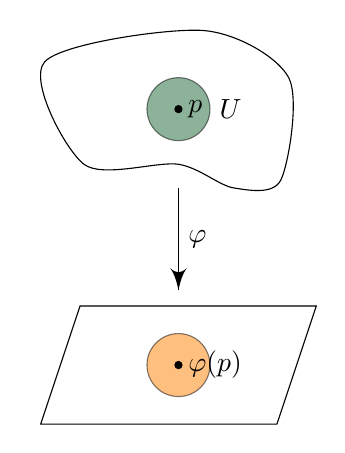
\begin{tikzpicture}
    \draw plot [smooth cycle] coordinates {(-1.2, -0.7) (0, -0.7) (0.7, -1) (1.3, -0.9) (1.4, 0.4) (0.3, 1) (-1.7, 0.6)};

    \draw [fill=mgreen, opacity=0.5] circle [radius=0.4];
    \node [right] {$p$};
    \node [circ] {};
    \node at (0.4, 0) [right] {$U$};

    \begin{scope}[shift={(-1.75, -4)}]
      \draw (0, 0) -- (3, 0) -- (3.5, 1.5) -- (0.5, 1.5) -- cycle;

      \draw (1.75, 0.75) [fill=morange, opacity=0.5] circle [radius=0.4];
      \node at (1.75, 0.75) [right] {$\varphi(p)$};
      \node at (1.75, 0.75) [circ] {};
    \end{scope}

    \draw [->] (0, -1) -- +(0, -1.3) node [pos=0.5, right] {$\varphi$};
  \end{tikzpicture}
\end{center}
With a chart, we can talk about things like continuity, differentiability by identifying $U$ with $\varphi(U)$:
\begin{defi}[Smooth function]\index{smooth function}\index{$C^\infty$}
  Let $(U, \varphi)$ be a chart on $M$ and $f: M \to \R$. We say $f$ is \emph{smooth} or $C^\infty$ at $p \in U$ if $f \circ \varphi^{-1}: \varphi(U) \to \R$ is smooth at $\varphi(p)$ in the usual sense.
  \[
    \begin{tikzcd}
      \R^n \supseteq \varphi(U) \ar[r, "\varphi^{-1}"] & U \ar[r, "f"] & \R
    \end{tikzcd}
  \]
\end{defi}
\begin{center}
  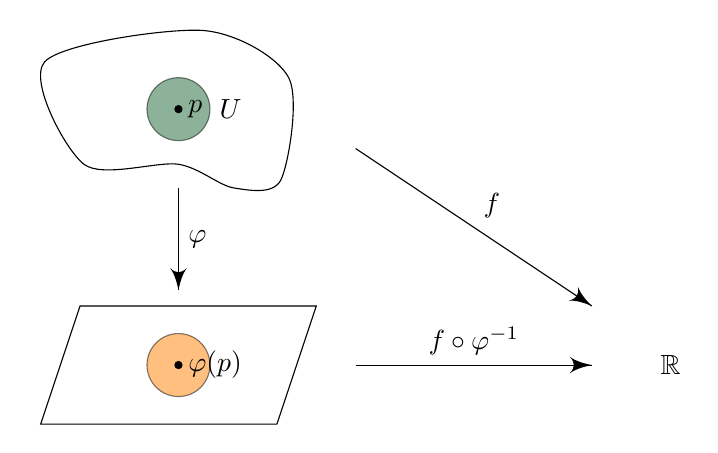
\begin{tikzpicture}
    \draw plot [smooth cycle] coordinates {(-1.2, -0.7) (0, -0.7) (0.7, -1) (1.3, -0.9) (1.4, 0.4) (0.3, 1) (-1.7, 0.6)};

    \draw [fill=mgreen, opacity=0.5] circle [radius=0.4];
    \node [right] {$p$};
    \node [circ] {};
    \node at (0.4, 0) [right] {$U$};

    \begin{scope}[shift={(-1.75, -4)}]
      \draw (0, 0) -- (3, 0) -- (3.5, 1.5) -- (0.5, 1.5) -- cycle;

      \draw (1.75, 0.75) [fill=morange, opacity=0.5] circle [radius=0.4];
      \node at (1.75, 0.75) [right] {$\varphi(p)$};
      \node at (1.75, 0.75) [circ] {};

      \draw [->] (4, 0.75) -- (7, 0.75) node [pos=0.5, above] {$f \circ \varphi^{-1}$};
      \node at (8, 0.75) {$\R$};
      \draw [->] (4, 3.5) -- (7, 1.5) node [pos=0.5, anchor = south west] {$f$};
    \end{scope}

    \draw [->] (0, -1) -- +(0, -1.3) node [pos=0.5, right] {$\varphi$};

  \end{tikzpicture}
\end{center}
We can define all other notions such as continuity, differentiability, twice differentiability etc.\ similarly.

This definition has a problem that some points might not be in the chart, and we don't know how to determine if a function is, say, smooth at the point. The solution is easy --- we just take many charts that together cover $M$. However, we have the problem that a function might be smooth at a point relative to some chart, but not relative to some other chart. The solution is to require the charts to be compatible in some sense.

\begin{defi}[Atlas]\index{atlas}
  An \emph{atlas} on a set $M$ is a collection of charts $\{(U_\alpha, \varphi_\alpha)\}$ on $M$ such that
  \begin{enumerate}
    \item $M = \bigcup_{\alpha} U_\alpha$.
    \item For all $\alpha, \beta$, we have $\varphi_\alpha(U_\alpha \cap U_\beta)$ is open in $\R^n$, and the transition function
      \[
        \varphi_\alpha \circ \varphi_\beta^{-1}: \varphi_\beta(U_\alpha \cap U_\beta) \to \varphi_\alpha(U_\alpha \cap U_\beta)
      \]
      is smooth (in the usual sense).
  \end{enumerate}
\end{defi}
\begin{center}
  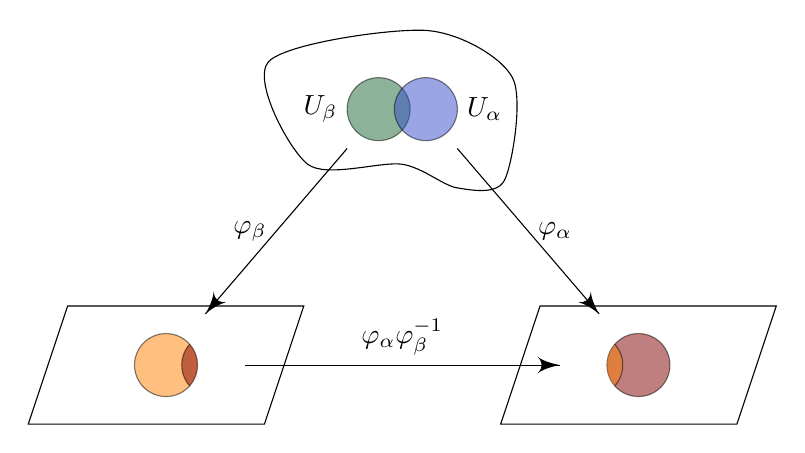
\begin{tikzpicture}
    \draw plot [smooth cycle] coordinates {(-1.2, -0.7) (0, -0.7) (0.7, -1) (1.3, -0.9) (1.4, 0.4) (0.3, 1) (-1.7, 0.6)};

    \draw (-0.3, 0) [fill=mgreen, opacity=0.5] circle [radius=0.4];
    \draw (0.3, 0) [fill=mblue, opacity=0.5] circle [radius=0.4];

    \node [left] at (-0.7, 0) {$U_\beta$};
    \node [right] at (0.7, 0) {$U_\alpha$};

    \begin{scope}[shift={(-4.75, -4)}]
      \draw (0, 0) -- (3, 0) -- (3.5, 1.5) -- (0.5, 1.5) -- cycle;

      \draw (1.75, 0.75) [fill=morange, opacity=0.5] circle [radius=0.4];
      \begin{scope}
        \clip (1.75, 0.75) circle [radius=0.4];
        \draw (2.35, 0.75) [fill=mred, opacity=0.5] circle [radius=0.4];
      \end{scope}
    \end{scope}

    \draw [->] (-0.7, -0.5) -- (-2.5, -2.6) node [pos=0.5, left] {$\varphi_\beta$};
    \draw [->] (0.7, -0.5) -- (2.5, -2.6) node [pos=0.5, right] {$\varphi_\alpha$};

    \begin{scope}[shift={(1.25, -4)}]
      \draw (0, 0) -- (3, 0) -- (3.5, 1.5) -- (0.5, 1.5) -- cycle;

      \draw (1.75, 0.75) [fill=mred, opacity=0.5] circle [radius=0.4];
      \begin{scope}
        \clip (1.75, 0.75) circle [radius=0.4];
        \draw (1.15, 0.75) [fill=morange, opacity=0.5] circle [radius=0.4];
      \end{scope}
    \end{scope}
    \draw [->] (-2, -3.25) -- (2, -3.25) node [pos=0.5, above] {$\varphi_\alpha \varphi_\beta^{-1}$};
  \end{tikzpicture}
\end{center}

\begin{lemma}
  If $(U_\alpha, \varphi_\alpha)$ and $(U_\beta, \varphi_\beta)$ are charts in some atlas, and $f: M \to \R$, then $f \circ \varphi_\alpha^{-1}$ is smooth at $\varphi_\alpha(p)$ if and only if $f \circ \varphi_\beta^{-1}$ is smooth at $\varphi_\beta (p)$ for all $p \in U_\alpha \cap U_\beta$.
\end{lemma}

\begin{proof}
  We have
  \[
    f \circ \varphi_\beta^{-1} = f \circ \varphi_\alpha^{-1} \circ (\varphi_\alpha \circ \varphi_\beta^{-1}). \qedhere
  \]
\end{proof}
So we know that if we have an atlas on a set, then the notion of smoothness does not depend on the chart.

\begin{eg}
  Consider the sphere
  \[
    S^2 = \{(x_1, x_2, x_3): \sum x_i^2 = 1\} \subseteq \R^3.
  \]
  We let
  \[
    U_1^+ = S^2 \cap \{x_1 > 0\},\quad U_1^- = S^2 \cap \{x_1 < 0\}, \cdots
  \]
  We then let
  \begin{align*}
    \varphi_1^+: U_1^+ &\to \R^2\\
    (x_1, x_2, x_3) &\mapsto (x_2, x_3).
  \end{align*}
  It is easy to show that this gives a bijection to the open disk in $\R^2$. We similarly define the other $\varphi_i^{\pm}$. These then give us an atlas of $S^2$.
\end{eg}

\begin{defi}[Equivalent atlases]\index{equivalent atlases}\index{atlas!equivalence}
  Two atlases $\mathcal{A}_1$ and $\mathcal{A}_2$ are \emph{equivalent} if $\mathcal{A}_1 \cup \mathcal{A}_2$ is an atlas.
\end{defi}
Then equivalent atlases determine the same smoothness, continuity etc.\ information.

\begin{defi}[Differentiable structure]\index{differentiable structure}
  A \emph{differentiable structure} on $M$ is a choice of equivalence class of atlases.
\end{defi}

We want to define a manifold to be a set with a differentiable structure. However, it turns out we can find some really horrendous sets that have differential structures.

\begin{eg}
  Consider the line with two origins given by taking $\R \times \{0\} \cup \R \times \{1\}$ and then quotienting by
  \[
    (x, 0) \sim (x, 1)\text{ for } x \not= 0.
  \]
  \begin{center}
    \begin{tikzpicture}
      \draw (-3, 0) -- (3, 0);
      \node [fill=white, draw, circle, inner sep=0, minimum size=3] {};
      \node [circ] at (0, 0.2) {};
      \node [circ] at (0, -0.2) {};
    \end{tikzpicture}
  \end{center}
  Then the inclusions of the two copies of $\R$ gives us an atlas of the space.
\end{eg}

The problem with this space is that it is not Hausdorff, which is bad. However, that is not actually true, because $M$ is not a topological space, so it doesn't make sense to ask if it is Hausdorff. So we want to define a topology on $M$, and then impose some topological conditions on our manifolds.

It turns out the smooth structure already gives us a topology:

\begin{ex}
  An atlas determines a topology on $M$ by saying $V \subseteq M$ is open iff $\varphi(U \cap V)$ is open in $\R^n$ for all charts $(U, \varphi)$ in the atlas. Equivalent atlases give the same topology.
\end{ex}

We now get to the definition of a manifold.

\begin{defi}[Manifold]\index{manifold}
  A \emph{manifold} is a set $M$ with a choice of differentiable structure whose topology is
  \begin{enumerate}
    \item Hausdorff\index{Hausdorff}, i.e.\ for all $x, y \in M$, there are open neighbourhoods $U_x, U_y \subseteq M$ with $x \in U_x, y \in U_y$ and $U_x \cap U_y = \emptyset$.
    \item Second countable\index{second countable}, i.e.\ there exists a countable collection $(U_n)_{n \in \N}$ of open sets in $M$ such that for all $V \subseteq M$ open, and $p \in V$, there is some $n$ such that $p \in U_n \subseteq V$.
  \end{enumerate}
\end{defi}
The second countability condition is a rather technical condition that we wouldn't really use much. This, for example, excludes the long line.

Note that we will often refer to a manifold simply as $M$, where the differentiable structure is understood from context. By a chart on $M$, we mean one in some atlas in the equivalence class of atlases.

\begin{defi}[Local coordinates]\index{local coordinates}
  Let $M$ be a manifold, and $\varphi: U \to \varphi(U)$ a chart of $M$. We can write
  \[
    \varphi = (x_1, \cdots, x_n)
  \]
  where each $x_i: U \to \R$. We call these the \emph{local coordinates}.
\end{defi}
So a point $p \in U$ can be represented by local coordinates
\[
  (x_1(p), \cdots, x_n(p)) \in \R^n.
\]
By abuse of notation, if $f: M \to \R$, we confuse $f|_U$ and $f \circ \varphi^{-1}: \varphi(U) \to \R$. So we write $f(x_1, \cdots, x_n)$ to mean $f(p)$, where $\varphi(p) = (x_1, \cdots, x_n) \in \varphi(U)$.
\[
  \begin{tikzcd}
    U \ar[r, hook, "\iota"] \ar[d, "\varphi"] & M \ar[r, "f"] & \R\\
    \varphi(U) \ar[rru, "f|_U"']
  \end{tikzcd}
\]
Of course, we can similarly define $C^0, C^1, C^2, \cdots$ manifolds, or analytic manifolds. We can also model manifolds on other spaces, e.g.\ $\C^n$, where we get complex manifolds, or on infinite-dimensional spaces.

\begin{eg}\leavevmode
  \begin{enumerate}
    \item Generalizing the example of the sphere, the $n$-dimensional sphere $S^n = \{(x_0, \cdots, x_n) \in \R^{n + 1}: \sum x_i^2 = 1\}$ is a manifold.
    \item If $M$ is open in $\R^n$, then the inclusion map $\varphi: M \to \R^n$ given by $\varphi(p) = p$ is a chart forming an atlas. So $M$ is a manifold. In particular, $\R^n$ is a manifold, with its ``standard'' differentiable structure. We will always assume $\R^n$ is given this structure, unless otherwise specified.
    \item $M(n, n)$, the set of all $n \times n$ matrices is also a manifold, by the usual bijection with $\R^{n^2}$. Then $\GL_n \subseteq M(n, n)$ is open, and thus also a manifold.
    \item The set $\RP^n$, the set of one-dimensional subspaces of $\R^{n + 1}$ is a manifold. We can define charts as follows: we let $U_i$ to be the lines spanned by a vector of the form $(v_0, v_1, \cdots, v_{i - 1}, 1, v_{i + 1}, \cdots, v_n) \in \R^{n + 1}$.

      We define the map $\varphi_i: U_i \to \R^n \cong \{\mathbf{x} \in \R^{n + 1}: x_i = 1\}$ that sends $\varphi(L) = (v_0, \cdots, 1, \cdots, v_n)$, where $L$ is spanned by $(v_0, \cdots, 1, \cdots, v_n)$. It is an easy exercise to show that this defines a chart.
  \end{enumerate}
\end{eg}

Note that when we defined a chart, we talked about charts as maps $U \to \R^n$. We did not mention whether $n$ is fixed, or whether it is allowed to vary. It turns out it cannot vary, as long as the space is connected.

\begin{lemma}
  Let $M$ be a manifold, and $\varphi_1: U_1 \to \R^n$ and $\varphi_2: U_2 \to \R^m$ be charts. If $U_1 \cap U_2 \not= \emptyset$, then $n = m$.
\end{lemma}

\begin{proof}
  We know
  \[
    \varphi_1 \varphi_2^{-1}: \varphi_2(U_1 \cap U_2) \to \varphi_1(U_1 \cap U_2)
  \]
  is a smooth map with inverse $\varphi_2 \varphi_1^{-1}$. So the derivative
  \[
    D(\varphi_1 \varphi_2^{-1})(\varphi_2(p)): \R^m \to \R^n
  \]
  is a linear isomorphism, whenever $p \in U_1 \cap U_2$. So $n = m$.
\end{proof}

\begin{defi}[Dimension]\index{dimension}
  If $p \in M$, we say $M$ has \emph{dimension} $n$ at $p$ if for one (thus all) charts $\varphi: U \to \R^m$ with $p \in U$, we have $m = n$. We say $M$ has dimension $n$ if it has dimension $n$ at all points.
\end{defi}

\subsection{Smooth functions and derivatives}
From now on, $M$ and $N$ will be manifolds. As usual, we would like to talk about maps between manifolds. What does it mean for such a map to be smooth? In the case of a function $M \to \R$, we had to check it on each chart of $M$. Now that we have functions $M \to N$, we need to check it on charts of \emph{both} $N$ and $M$.

\begin{defi}[Smooth function]\index{smooth function}
  A function $f: M \to N$ is \emph{smooth at a point $p \in M$} if there are charts $(U, \varphi)$ for $M$ and $(V, \xi)$ for $N$ with $p \in U$ and $f(p) \in V$ such that $\xi \circ f \circ \varphi^{-1}: \varphi(U) \to \xi(V)$ is smooth at $\varphi(p)$.

  A function is \emph{smooth} if it is smooth at all points $p \in M$.

  A \term{diffeomorphism} is a smooth $f$ with a smooth inverse.

  We write $C^\infty(M, N)$ \index{$C^\infty(M, N)$} for the space of smooth maps $f: M \to N$. We write $C^\infty(M)$\index{$C^\infty(M)$} for $C^\infty(M, \R)$, and this has the additional structure of an algebra, i.e.\ a vector space with multiplication.
\end{defi}
\begin{center}
  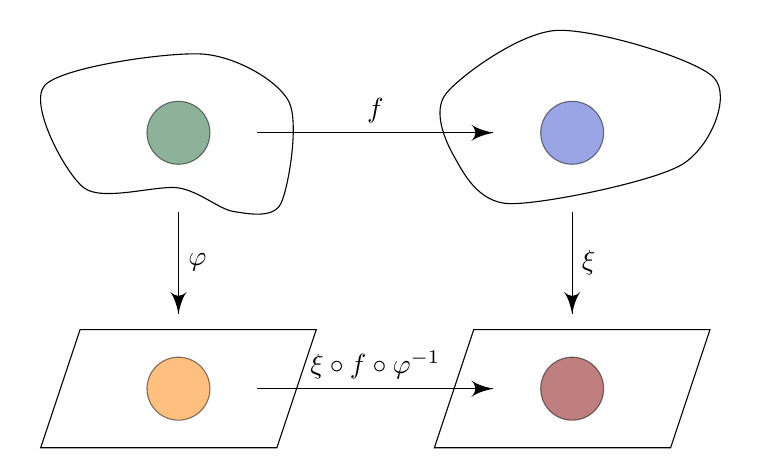
\begin{tikzpicture}
    \draw plot [smooth cycle] coordinates {(-1.2, -0.7) (0, -0.7) (0.7, -1) (1.3, -0.9) (1.4, 0.4) (0.3, 1) (-1.7, 0.6)};

    \draw [fill=mgreen, opacity=0.5] circle [radius=0.4];

    \begin{scope}[shift={(-1.75, -4)}]
      \draw (0, 0) -- (3, 0) -- (3.5, 1.5) -- (0.5, 1.5) -- cycle;

      \draw (1.75, 0.75) [fill=morange, opacity=0.5] circle [radius=0.4];
    \end{scope}

    \draw [->] (0, -1) -- +(0, -1.3) node [pos=0.5, right] {$\varphi$};
    \begin{scope}[shift={(5, 0)}]
      \draw plot [smooth cycle] coordinates {(1.4, -0.4) (-0.8, -0.9) (-1.5, -0.3) (-1.6, 0.5) (-0.2, 1.3) (1.8, 0.7)};

      \draw [fill=mblue, opacity=0.5] circle [radius=0.4];

      \begin{scope}[shift={(-1.75, -4)}]
        \draw (0, 0) -- (3, 0) -- (3.5, 1.5) -- (0.5, 1.5) -- cycle;

        \draw (1.75, 0.75) [fill=mred, opacity=0.5] circle [radius=0.4];
      \end{scope}

      \draw [->] (0, -1) -- +(0, -1.3) node [pos=0.5, right] {$\xi$};
    \end{scope}

    \draw [->] (1, 0) -- (4, 0) node [above, pos=0.5] {$f$};

    \draw [->] (1, -3.25) -- (4, -3.25) node [above, pos=0.5] {$\xi \circ f \circ \varphi^{-1}$};
  \end{tikzpicture}
\end{center}
Equivalently, $f$ is smooth at $p$ if $\xi \circ f \circ \varphi^{-1}$ is smooth at $\varphi(p)$ for \emph{any} such charts $(U, \varphi)$ and $(V, \xi)$.

\begin{eg}
  Let $\varphi: U \to \R^n$ be a chart. Then $\varphi: U \to \varphi(U)$ is a diffeomorphism.
\end{eg}

\begin{defi}[Curve]\index{curve}
  A \emph{curve} is a smooth map $I \to M$, where $I$ is a non-empty open interval.
\end{defi}

To discuss derivatives, we first look at the case where $U \subseteq \R^n$ is open. Suppose $f: U \to \R$ is smooth. If $p \in U$ and $\mathbf{v} \in \R^n$, recall that the \term{directional derivative} is defined by
\[
  Df|_p(\mathbf{v}) = \lim_{t \to 0} \frac{f(p + t\mathbf{v}) - f(p)}{t}.
\]
If $\mathbf{v} = \mathbf{e}_i = (0, \cdots, 0, 1, 0, \cdots, 0)$, then we write
\[
  Df|_p (\mathbf{e}_i) = \left.\frac{\partial f}{\partial x_i}\right|_p.
\]
Also, we know $Df|_p: \R^n \to \R$ is a linear map (by definition of smooth).

Note that here $p$ and $\mathbf{v}$ are both vectors, but they play different roles --- $p$ is an element in the domain $U$, while $\mathbf{v}$ is an arbitrary vector in $\R^n$. Even if $\mathbf{v}$ is enormous, by taking a small enough $t$, we find that $p + t\mathbf{v}$ will eventually be inside $U$.

If we have a general manifold, we can still talk about the $p$. However, we don't have anything that plays the role of a vector. Our first goal is to define the tangent space to a manifold that captures where the ``directions'' live.

An obvious way to do so would be to use a curve. Suppose $\gamma: I \to M$ is a curve, with $\gamma(0) = p \in U \subseteq M$, and $f: U \to \R$ is smooth. We can then take the derivative of $f$ along $\gamma$ as before. We let
\[
  X(f) = \left.\frac{\d}{\d t}\right|_{t = 0} f(\gamma(t)).
\]
It is an exercise to see that $X: C^\infty(U) \to \R$ is a linear map, and it satisfies the \term{Leibniz rule}
\[
  X(fg) = f(p) X(g) + g(p) X(f).
\]
We denote $X$ by $\dot{\gamma}(0)$. We might think of defining the tangent space as curves up to some equivalence relation, but if we do this, there is no obvious vector space on it. The trick is to instead define a vector by the derivative $X$ induces. This then has an obvious vector space structure.
\begin{defi}[Derivation]\index{derivation}
  A \emph{derivation} on an open subset $U \subseteq M$ at $p \in U$ is a linear map $X: C^\infty(U) \to \R$ satisfying the Leibniz rule
  \[
    X(fg) = f(p) X(g) + g(p) X(f).
  \]
\end{defi}

\begin{defi}[Tangent space]\index{tangent space}
  Let $p \in U \subseteq M$, where $U$ is open. The \emph{tangent space} of $M$ at $p$ is the vector space
  \[
    T_p M = \{ \, \text{derivations on $U$ at $p$} \, \} \equiv \Der_p(C^\infty(U)).
  \]
  The subscript $p$ tells us the point at which we are taking the tangent space.
\end{defi}
Why is this the ``right'' definition? There are two things we would want to be true:
\begin{enumerate}
  \item The definition doesn't actually depend on $U$.
  \item This definition agrees with the usual definition of tangent vectors in $\R^n$.
\end{enumerate}
We will do the first part at the end by bump functions, and will do the second part now. Note that it follows from the second part that every tangent vector comes from the derivative of a path, because this is certainly true for the usual definition of tangent vectors in $\R^n$ (take a straight line), and this is a completely local problem.

\begin{eg}\index{$\frac{\partial}{\partial x_i}$}
  Let $U \subseteq \R^n$ be open, and let $p \in U$. Then we have tangent vectors
  \[
    \left.\frac{\partial}{\partial x_i}\right|_p \in T_p \R^n, \qquad i = 1, \ldots, n.
  \]
  These correspond to the canonical basis vectors in $\R^n$.
\end{eg}

\begin{lemma}
  $\left.\frac{\partial}{\partial x_1}\right|_p, \cdots, \left.\frac{\partial}{\partial x_n}\right|_p$ is a basis of $T_p \R^n$. So these are all the derivations.
\end{lemma}

The idea of the proof is to show that a derivation can only depend on the first order derivatives of a function, and all possibilities will be covered by the $\frac{\partial}{\partial x_i}$.

\begin{proof}
  Independence is clear as
  \[
    \frac{\partial x_j}{\partial x_i} = \delta_{ij}.
  \]
  We need to show spanning. For notational convenience, we wlog take $p = 0$. Let $X \in T_0 \R^n$.

  We first show that if $g \in C^\infty(U)$ is the constant function $g = 1$, then $X(g) = 0$. Indeed, we have
  \[
    X(g) = X(g^2) = g(0) X(g) + X(g) g(0) = 2 X(g).
  \]
  Thus, if $h$ is any constant function, say, $c$, then $X(h) = X(cg) = c X(g)$. So the derivative of any constant function vanishes.

  In general, let $f \in C^\infty(U)$. By Taylor's theorem, we have
  \[
    f(x_1, \cdots, x_n) = f(0) + \sum_{i = 1}^n \left.\frac{\partial f}{\partial x_i}\right|_0 x_i + \varepsilon,
  \]
  where $\varepsilon$ is a sum of terms of the form $x_i x_j h$ with $h \in C^\infty(U)$.

  We set $\lambda_i = X(x_i) \in \R$. We first claim that $X(\varepsilon) = 0$. Indeed, we have
  \[
    X (x_i x_j h) = x_i(0) X(x_j h) + (x_jh)(0) X(x_i) = 0.
  \]
  So we have
  \[
    X(f) = \sum_{i = 1}^n \lambda_i \left.\frac{\partial f}{\partial x_i}\right|_0.
  \]
  So we have
  \[
    X = \sum_{i = 1}^n \lambda_i \left.\frac{\partial}{\partial x_i}\right|_0. \qedhere
  \]
\end{proof}

Given this definition of a tangent vector, we have a rather silly and tautological definition of the derivative of a smooth function.
\begin{defi}[Derivative]\index{derivative}
  Suppose $F \in C^\infty(M, N)$, say $F(p) = q$. We define $\D F|_p: T_p M \to T_q N$ by
  \[
    \D F|_p(X)(g) = X(g \circ F)
  \]
  for $X \in T_pM$ and $g \in C^\infty(V)$ with $q \in V \subseteq N$.

  This is a linear map called the \emph{derivative} of $F$ at $p$.
  \[
    \begin{tikzcd}
      M \ar[r, "F"] \ar[rd, "g \circ F"'] & N \ar[d, "g"]\\
      & \R
    \end{tikzcd}
  \]
\end{defi}

With a silly definition of a derivative comes a silly definition of the chain rule.
\begin{prop}[Chain rule]\index{chain rule}
  Let $M, N, P$ be manifolds, and $F \in C^\infty(M, N)$, $G \in C^\infty(N, P)$, and $p \in M, q = F(p)$. Then we have
  \[
    \D(G \circ F)|_p = \D G|_q \circ \D F|_p.
  \]
\end{prop}

\begin{proof}
  Let $h \in C^\infty(P)$ and $X \in T_p M$. We have
  \[
    \D G|_q (\D F|_p (X))(h) = \D F|_p(X) (h \circ G) = X(h \circ G \circ F) = \D (G \circ F)|_p (X)(h). \qedhere
  \]
\end{proof}
Note that this does not provide a new, easy proof of the chain rule. Indeed, to come this far into the course, we have used the actual chain rule something like ten thousand times.

\begin{cor}
  If $F$ is a diffeomorphism, then $\D F|_p$ is a linear isomorphism, and $(\D F|_p)^{-1} = \D (F^{-1})|_{F(p)}$.
\end{cor}

In the special case where the domain is $\R$, there is a canonical choice of tangent vector at each point, namely $1$.
\begin{defi}[Derivative]\index{derivative}
  Let $\gamma: \R \to M$ be a smooth function. Then we write
  \[
    \frac{\d \gamma}{\d t}(t) = \dot{\gamma}(t) = \D \gamma|_t (1).
  \]
\end{defi}

We now go back to understanding what $T_pM$ is if $p \in M$. We let $p \in U$ where $(U, \varphi)$ is a chart. Then if $q = \varphi(p)$, the map $\D\varphi|_p: T_p M \to T_q \R^n$ is a linear isomorphism.

\begin{defi}[$\frac{\partial}{\partial x_i}$]\index{$\frac{\partial}{\partial x_i}$}
  Given a chart $\varphi: U \to \R^n$ with $\varphi = (x_1, \cdots, x_n)$, we define
  \[
    \left.\frac{\partial}{\partial x_i}\right|_p = (\D \varphi|_p)^{-1} \left(\left.\frac{\partial}{\partial x_i}\right|_{\varphi(p)}\right) \in T_p M.
  \]
\end{defi}
So $\left.\frac{\partial}{\partial x_1}\right|_p, \cdots, \left.\frac{\partial}{\partial x_n}\right|_p$ is a basis for $T_p M$.

Recall that if $f: U \to \R$ is smooth, then we can write $f(x_1, \cdots, x_n)$. Then we have
\[
  \left.\frac{\partial}{\partial x_i}\right|_p (f) = \left.\frac{\partial f}{\partial x_i}\right|_{\varphi(p)}.
\]
So we have a consistent notation.

Now, how does this basis change when we change coordinates? Suppose we also have coordinates $y_1, \cdots, y_n$ near $p$ given by some other chart. We then have $\left.\frac{\partial}{\partial y_i}\right|_p \in T_p M$. So we have
\[
  \left.\frac{\partial}{\partial y_i}\right|_p = \sum_{j = 1}^n \alpha_j \left.\frac{\partial}{\partial x_j}\right|_p
\]
for some $\alpha_j$. To figure out what they are, we apply them to the function $x_k$. So we have
\[
  \left.\frac{\partial}{\partial y_i}\right|_p (x_k) = \frac{\partial x_k}{\partial y_i}(p) = \alpha_k.
\]
So we obtain
\[
  \left.\frac{\partial}{\partial y_i}\right|_p = \sum_{j = 1}^n \frac{\partial x_j}{\partial y_i}(p)\left.\frac{\partial}{\partial x_j}\right|_p.
\]
This is the usual change-of-coordinate formula!

Now let $F \in C^\infty(M, N)$, $(U, \varphi)$ be a chart on $M$ containing $p$ with coordinates $x_1, \cdots, x_n$, and $(V, \xi)$ a chart on $N$ containing $q = F(p)$ with coordinates $y_1,\cdots, y_m$. By abuse of notation, we confuse $F$ and $\xi \circ F \circ \varphi^{-1}$. So we write $F = (F_1, \cdots, F_m)$ with $F_i = F_i(x_1, \cdots, x_n): U \to \R$.

As before, we have a basis
\begin{align*}
  \left.\frac{\partial}{\partial x_1}\right|_p, \cdots, \left.\frac{\partial}{\partial x_n}\right|_p&\quad\text{for}\quad T_pM,\\
  \left.\frac{\partial}{\partial y_1}\right|_q, \cdots, \left.\frac{\partial}{\partial y_m}\right|_q&\quad\text{for}\quad T_qN.
\end{align*}

\begin{lemma}
  We have
  \[
    \D F|_p \left(\left.\frac{\partial}{\partial x_i}\right|_p\right) = \sum_{j = 1}^m \frac{\partial F_j}{\partial x_i}(p) \left.\frac{\partial}{\partial y_j}\right|_q.
  \]
  In other words, $\D F|_p$ has matrix representation
  \[
    \left(\frac{\partial F_j}{\partial x_i}(p)\right)_{ij}.
  \]
\end{lemma}

\begin{proof}
  We let
  \[
    \D F|_p \left(\left.\frac{\partial}{\partial x_i}\right|_p\right) = \sum_{j = 1}^m \lambda_j \left.\frac{\partial}{\partial y_j}\right|_q.
  \]
  for some $\lambda_j$. We apply this to the local function $y_k$ to obtain
  \begin{align*}
    \lambda_k &= \left(\sum_{j = 1}^m \lambda_j \left.\frac{\partial}{\partial y_j}\right|_q\right)(y_k)\\
    &= \D F_p \left(\left.\frac{\partial}{\partial x_i}\right|_p\right)(y_k)\\
    &= \left.\frac{\partial}{\partial x_i}\right|_p (y_k \circ F) \\
    &= \left.\frac{\partial}{\partial x_i}\right|_p(F_k) \\
    &= \frac{\partial F_k}{\partial x_i}(p). \qedhere
  \end{align*}
\end{proof}

\begin{eg}
  Let $f: C^\infty(U)$ where $U \subseteq M$ is an open set containing $p$. Then $\D f|_p: T_p M \to T_{f(p)} \R \cong \R$ is a linear map. So $\D f|_p$ is an element in the dual space $(T_pM)^*$, called the \term{differential} of $f$ at $p$, and is denoted $\d f|_p$. Then we have
  \[
    \d f|_p(X) = X(f).
  \]
  (this can, e.g.\ be checked in local coordinates)
\end{eg}

\subsection{Bump functions and partitions of unity}
Recall that there is one thing we swept under the carpet --- to define the tangent space, we needed to pick an open set $U$. Ways to deal with this can be found in the example sheet, but there are two general approaches --- one is to talk about germs of functions, where we consider all open neighbourhoods, and identify two functions if they agree on some open neighbourhood of the point. The other way is to realize that we can ``extend'' any function on $U \subseteq M$ to a function on the whole of $M$, using bump functions.

In general, we want a function that looks like this:
\begin{center}
  \begin{tikzpicture}
    \draw [->] (-3, 0) -- (3, 0);
    \draw [->] (0, -0.5) -- (0, 3);
    \draw [thick, blue] (-1.01, 2) -- (1.01, 2);
    \draw [thick, blue] (-3, 0) -- (-1.99, 0);
    \draw [thick, blue] (1.99, 0) -- (3, 0);
    \draw [domain=-1.99:-1.01, thick, blue] plot [smooth] (\x, {2 * (exp(- 1 / ((2 + \x) * (2 + \x))))/((exp(- 1 / ((2 + \x) * (2 + \x)))) + (exp(- 1 / ((-1 - \x) * (-1 - \x)))))});
    \draw [domain=1.01:1.99, thick, blue] plot [smooth] (\x, {2 * (exp(- 1 / ((2 - \x) * (2 - \x))))/((exp(- 1 / ((2 - \x) * (2 - \x)))) + (exp(- 1 / ((-1 + \x) * (-1 + \x)))))});
  \end{tikzpicture}
\end{center}

\begin{lemma}
  Suppose $W \subseteq M$ is a coordinate chart with $p \in W$. Then there is an open neighbourhood $V$ of $p$ such that $\bar{V} \subseteq W$ and an $X \in C^\infty(M, \R)$ such that $X = 1$ on $V$ and $X = 0$ on $M \setminus W$.
\end{lemma}

\begin{proof}
  Suppose we have coordinates $x_1, \cdots, x_n$ on $W$. We wlog suppose these are defined for all $|x| < 3$.

  We define $\alpha, \beta, \gamma: \R \to \R$ by
  \[
    \alpha(t) =
    \begin{cases}
      e^{-t^{-2}} & t > 0\\
      0 & t \leq 0
    \end{cases}.
  \]
  \begin{center}
    \begin{tikzpicture}
      \draw [->] (-3, 0) -- (3, 0);
      \draw [->] (0, -0.5) -- (0, 3);
      \draw [thick, blue] (-3, 0) -- (0, 0);
      \draw [domain=0.01:3, thick, blue] plot [smooth] (\x, {2 * exp(- 1 / (\x * \x))});
    \end{tikzpicture}
  \end{center}
  We now let
  \[
    \beta(t) = \frac{\alpha(t)}{\alpha(t) + \alpha(1 - t)}.
  \]
  \begin{center}
    \begin{tikzpicture}[xscale=4]
      \draw [->] (0, 0) -- (1, 0);
      \draw [->] (0, -0.5) -- (0, 3);
      \draw [thick, blue] (0, 0) -- (0.01, 0);
      \draw [domain=0.01:0.99, thick, blue] plot [smooth] (\x, {2 * (exp(- 1 / (\x * \x)))/((exp(- 1 / (\x * \x))) + (exp(- 1 / ((1 - \x) * (1 - \x)))))});
    \end{tikzpicture}
  \end{center}
  Then we let
  \[
    \gamma(t) = \beta(t + 2)\beta(2 - t).
  \]
  \begin{center}
    \begin{tikzpicture}
      \draw [->] (-3, 0) -- (3, 0);
      \draw [->] (0, -0.5) -- (0, 3);
      \draw [thick, blue] (-1.01, 2) -- (1.01, 2);
      \draw [thick, blue] (-3, 0) -- (-1.99, 0);
      \draw [thick, blue] (1.99, 0) -- (3, 0);
      \draw [domain=-1.99:-1.01, thick, blue] plot [smooth] (\x, {2 * (exp(- 1 / ((2 + \x) * (2 + \x))))/((exp(- 1 / ((2 + \x) * (2 + \x)))) + (exp(- 1 / ((-1 - \x) * (-1 - \x)))))});
      \draw [domain=1.01:1.99, thick, blue] plot [smooth] (\x, {2 * (exp(- 1 / ((2 - \x) * (2 - \x))))/((exp(- 1 / ((2 - \x) * (2 - \x)))) + (exp(- 1 / ((-1 + \x) * (-1 + \x)))))});
    \end{tikzpicture}
  \end{center}
  Finally, we let
  \[
    X(x_1, \cdots, x_n) = \gamma(x_1) \cdots \gamma(x_n).
  \]
  on $W$. We let
  \[
    V = \{\mathbf{x}: |x_i| < 1\}.
  \]
  Extending $X$ to be identically $0$ on $M \setminus W$ to get the desired smooth function (up to some constant).
\end{proof}
\begin{lemma}
  Let $p \in W \subseteq U$ and $W, U$ open. Let $f_1, f_2 \in C^\infty(U)$ be such that $f_1 = f_2$ on $W$. If $X \in \Der_p(C^\infty(U))$, then we have $X(f_1) = X(f_2)$
\end{lemma}

\begin{proof}
  Set $h = f_1 - f_2$. We can wlog assume that $W$ is a coordinate chart. We pick a bump function $\chi \in C^\infty(U)$ that vanishes outside $W$. Then $\chi h = 0$. Then we have
  \[
    0 = X(\chi h) = \chi(p) X(h) + h(p) X(\chi) = X(h) + 0 = X(f_1) - X(f_2). \qedhere
  \]
\end{proof}

While we're doing boring technical work, we might as well do the other one, known as a \emph{partition of unity}. The idea is as follows --- suppose we want to construct a global structure on our manifold, say a (smoothly varying) inner product for each tangent space $T_p M$. We know how to do this if $M = \R^n$, because there is a canonical choice of inner product at each point in $\R^n$. We somehow want to patch all of these together.

In general, there are two ways we can do the patching. The easy case is that not only is there a choice on $\R^n$, but there is a \emph{unique} choice. In this case, just doing it on each chart suffices, because they must agree on the intersection by uniqueness.

However, this is obviously not the case for us, because a vector space can have many distinct inner products. So we need some way to add them up.

\begin{defi}[Partition of unity]\index{partition of unity}
  Let $\{U_\alpha\}$ be an open cover of a manifold $M$. A \emph{partition of unity} subordinate to $\{U_\alpha\}$ is a collection $\varphi_\alpha \in C^\infty(M, \R)$ such that
  \begin{enumerate}
    \item $0 \leq \varphi_\alpha \leq 1$
    \item $\supp(\varphi_\alpha) \subseteq U_\alpha$
    \item For all $p \in M$, all but finitely many $\varphi_\alpha(p)$ are zero.
    \item $\sum_\alpha \varphi_\alpha = 1$.
  \end{enumerate}
\end{defi}
Note that by (iii), the final sum is actually a finite sum, so we don't have to worry about convergence issues.

Now if we have such a partition of unity, we can pick an inner product on each $U_\alpha$, say $q_\alpha(\ph, \ph)$, and then we can define an inner product on the whole space by
\[
  q(v_p, w_p) = \sum_{\alpha} \varphi_{\alpha}(p) q_\alpha(v_p, w_p),
\]
where $v_p, w_p \in T_p M$ are tangent vectors. Note that this makes sense. While each $q_\alpha$ is not defined everywhere, we know $\varphi_\alpha(p)$ is non-zero only when $q_\alpha$ is defined at $p$, and we are also only taking a finite sum.

The important result is the following:
\begin{thm}
  Given any $\{U_\alpha\}$ open cover, there exists a partition of unity subordinate to $\{U_\alpha\}$.
\end{thm}

\begin{proof}
  We will only do the case where $M$ is compact. Given $p \in M$, there exists a coordinate chart $p \in V_p$ and $\alpha(p)$ such that $V_p \subseteq U_{\alpha(p)}$. We pick a bump function $\chi_p \in C^\infty(M, \R)$ such that $\chi_p = 1$ on a neighbourhood $W_p \subseteq V_p$ of $p$. Then $\supp(\chi_p) \subseteq U_{\alpha(p)}$.

  Now by compactness, there are some $p_1, \cdots, p_N$ such that $M$ is covered by $W_{p_1} \cup \cdots \cup W_{p_N}$. Now let
  \[
    \tilde{\varphi}_\alpha = \sum_{i: \alpha(p_i) = \alpha} \chi_{p_i}.
  \]
  Then by construction, we have
  \[
    \supp(\tilde{\varphi}_\alpha) \subseteq U_\alpha.
  \]
  Also, by construction, we know $\sum_\alpha \tilde{\varphi}_\alpha > 0$. Finally, we let
  \[
    \varphi_\alpha = \frac{\tilde{\varphi}_\alpha}{\sum_\beta \tilde{\varphi}_\beta}. \qedhere
  \]
\end{proof}
The general proof will need the fact that the space is second-countable.

We will actually not need this until quite later on in the course, but we might as well do all the boring technical bits all together.

\subsection{Submanifolds}
You have a manifold, and a subset of it is a manifold, so you call it a submanifold.

\begin{defi}[Embedded submanifold]\index{Embedded submanifold}
  Let $M$ be a manifold with $\dim M = n$, and $S$ be a submanifold of $M$. We say $S$ is an \emph{embedded submanifold} if for all $p \in S$, there are coordinates $x_1, \cdots, x_n$ on some chart $U \subseteq M$ containing $p$ such that
  \[
    S \cap U = \{x_{k + 1} = x_{k + 2} = \cdots = x_n = 0\}
  \]
  for some $k$. Such coordinates are known as \term{slice coordinates} for $S$.
\end{defi}
This is a rather technical condition, rather than ``a subset that is also a manifold under the inherited smooth structure''. The two definitions are indeed equivalent, but picking this formulation makes it easier to prove things about it.

\begin{lemma}
  If $S$ is an embedded submanifold of $M$, then there exists a unique differential structure on $S$ such that the inclusion map $\iota: S \hookrightarrow M$ is smooth and $S$ inherits the subspace topology.
\end{lemma}

\begin{proof}
  Basically if $x_1, \cdots, x_n$ is a slice chart for $S$ in $M$, then $x_1, \cdots, x_k$ will be coordinates on $S$.

  More precisely, let $\pi: \R^n \to \R^k$ be the projection map
  \[
    \pi(x_1, \cdots, x_n) = (x_1, \cdots, x_k).
  \]
  Given a slice chart $(U, \varphi)$ for $S$ in $M$, consider $\tilde{\varphi}: S \cap U \to \R^k$ by $\tilde{\varphi} = \pi \circ \varphi$. This is smooth and bijective, and is so a chart on $S$. These cover $S$ by assumption. So we only have to check that the transition functions are smooth.

  Given another slice chart $(V, \xi)$ for $S$ in $M$, we let $\tilde{\xi} = \pi \circ \xi$, and check that
  \[
    \tilde{\xi} \circ \tilde{\varphi}^{-1} = \pi \circ \xi \circ \varphi^{-1} \circ j,
  \]
  where $j: \R^k \to \R^n$ is given by $j(x_1, \cdots, x_k) = (x_1, \cdots, x_k, 0, \cdots, 0)$.

  From this characterization, by looking at local charts, it is clear that $S$ has the subspace topology. It is then easy to see that the embedded submanifold is Hausdorff and second-countable, since these properties are preserved by taking subspaces.

  We can also check easily that $\iota: S \hookrightarrow M$ is smooth, and this is the only differential structure with this property.
\end{proof}

It is also obvious from the slice charts that:
\begin{prop}
  Let $S$ be an embedded submanifold. Then the derivative of the inclusion map $\iota: S \hookrightarrow M$ is injective.
\end{prop}

Sometimes, we like to think of a subobject not as a subset, but as the inclusion map $\iota: S \hookrightarrow M$ instead. However, when we are doing topology, there is this funny problem that a continuous bijection need not be a homeomorphism. So if we define submanifolds via inclusions maps, we get a weaker notion known as an \emph{immersed submanifold}.

\begin{defi}[Immersed submanifold]\index{immersed submanifold}
  Let $S, M$ be manifolds, and $\iota: S \hookrightarrow M$ be a smooth injective map with $\D\iota|_p : T_p S \to T_p M$ injective for all $p \in S$. Then we call $(\iota, S)$ an \emph{immersed submanifold}. By abuse of notation, we identify $S$ and $\iota(S)$.
\end{defi}

\begin{eg}
  If we map $\R$ into $\R^2$ via the following figure of eight (where the arrow heads denote the ``end points'' of $\R$), then this gives an immersed submanifold that is not an embedded submanifold.
  \begin{center}
    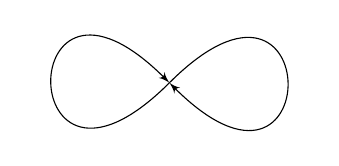
\begin{tikzpicture}
      \path[use as bounding box] (-1.8, -0.7) rectangle (1.8,0.7);
      \draw [-latex'] (0, 0) .. controls (2, 2) and (2, -2) .. (0, 0);
      \draw [-latex'] (0, 0) .. controls (-2, -2) and (-2, 2) .. (0, 0);
    \end{tikzpicture}
  \end{center}
\end{eg}

\begin{eg}
  Consider the line $\R$, and define the map $f: \R \to T^2 = \R^2 / \Z^2$ by $f(x) = \alpha x$, where $\alpha$ is some irrational number. Then this map gives an immersed submanifold of $T^2$, but is not an embedded submanifold, since $\R$ certainly does not have the subspace topology from $T^2$.
\end{eg}

How do we construct submanifolds? The definition is rather difficult to work with. It is not immediately clear whether
\[
  S^n = \{\mathbf{x} \in \R^{n + 1}: |\mathbf{x}| \leq 1\} \subseteq \R^{n + 1}
\]
is an embedded submanifold, even though it feels like it should be.

More generally, if $M, N$ are manifolds, $F \in C^\infty(M, N)$ and $c \in N$, under what circumstances will $F^{-1}(c)$ be an embedded submanifold of $M$? The answer is that $c$ has to be a regular value.
\begin{defi}[Regular value]\index{regular value}
  Let $F \in C^\infty(M, N)$ and $c \in N$. Let $S = F^{-1}(c)$. We say $c$ is a \emph{regular value} if for all $p \in S$, the map $\D F|_p: T_p M \to T_c N$ is surjective.
\end{defi}

\begin{prop}
  Let $F \in C^\infty(M, N)$, and let $c \in N$. Suppose $c$ is a regular value. Then $S = F^{-1}(c)$ is an embedded submanifold of dimension $\dim M - \dim N$.
\end{prop}

\begin{proof}
  We let $n = \dim M$ and $m = \dim N$. Notice that for the map $\D F$ to be surjective, we must have $n \geq m$.

  Let $p \in S$, so $F(p) = c$. We want to find a slice coordinate for $S$ near $p$. Since the problem is local, by restricting to local coordinate charts, we may wlog assume $N = \R^m$, $M = \R^n$ and $c = p = 0$.

  Thus, we have a smooth map $F: \R^n \to \R^m$ with surjective derivative at $0$. Then the derivative is
  \[
    \left(\left.\frac{\partial F_j}{\partial x_i}\right|_0\right)_{i = 1, \ldots, n; \, j = 1, \ldots, m},
  \]
  which by assumption has rank $m$. We reorder the $x_i$ so that the first $m$ columns are independent. Then the $m \times m$ matrix
  \[
    R = \left(\left.\frac{\partial F_j}{\partial x_i}\right|_0\right)_{i,j = 1, \ldots, m}
  \]
  is non-singular. We consider the map
  \[
    \alpha(x_1, \cdots, x_n) = (F_1, \cdots, F_m, x_{m + 1}, \cdots, x_n).
  \]
  We then obtain
  \[
    \D \alpha|_0 =
    \begin{pmatrix}
      R & * \\
      0 & I
    \end{pmatrix},
  \]
  and this is non-singular. By the inverse function theorem, $\alpha$ is a local diffeomorphism. So there is an open $W\subseteq \R^n$ containing $0$ such that $\alpha|_W: W \to \alpha(W)$ is smooth with smooth inverse. We claim that $\alpha$ is a slice chart of $S$ in $\R^n$.

  Since it is a smooth diffeomorphism, it is certainly a chart. Moreover, by construction, the points in $S$ are exactly those whose image under $F$ have the first $m$ coordinates vanish. So this is the desired slice chart.
\end{proof}

\begin{eg}
  We want to show that $S^n$ is a manifold. Let $F: \R^{n + 1} \to \R$ be defined by
  \[
    F(x_0, \cdots, x_n) = \sum x_i^2.
  \]
  Then $F^{-1}(1) = S^n$. We find that
  \[
    \D F|_p = 2(x_0, \cdots, x_n) \not= 0
  \]
  when $p \in S^n$. So $S^n$ is a manifold.
\end{eg}

\begin{eg}
  Consider the orthogonal group. We let $M_n \cong \R^{n^2}$ be the space of all $n \times n$ matrices with the obvious smooth structure. We define
  \[
    N = \{A \in M_n: A^T = A\}.
  \]
  Since this is a linear subspace, it is also a manifold. We define
  \begin{align*}
    F: M_n &\to N\\
    A &\mapsto AA^T.
  \end{align*}
  Then we have
  \[
    \Or(n) = F^{-1}(I) = \{A: AA^T = I\}.
  \]
  We compute the derivative by looking at
  \[
    F (A + H) = (A + H)(A + H)^T = AA^T + HA^T + AH^T + HH^T.
  \]
  So we have
  \[
    \D F|_A (H) = HA^T + AH^T.
  \]
  Now if $A \in \Or(n)$, then we have
  \[
    \D F|_A (HA) = HAA^T + AA^T H^T = H + H^T
  \]
  for any $H$. Since every symmetric matrix is of the form $H + H^T$, we know $\D F|_A: T_A M_n \to T_{F(A)}N$ is surjective. So $\Or(n)$ is a manifold.
\end{eg}

\section{Vector fields}
\subsection{The tangent bundle}
Recall that we had the notion of a tangent vector. If we have a curve $\gamma: I \to M$, then we would like to think that the derivative $\dot{\gamma}$ ``varies smoothly'' with time. However, we cannot really do that yet, since for different $t$, the value of $\dot{\gamma}$ lies in different vector spaces, and there isn't a way of comparing them.

More generally, given a ``vector field'' $f: p \mapsto v_p \in T_p M$ for each $p \in M$, how do we ask if this is a smooth function?

One way to solve this is to pick local coordinates $x_1, \cdots,x _n$ on $U \subseteq M$. We can then write
\[
  v_p = \sum_i \alpha_i(p) \left.\frac{\partial}{\partial x_i}\right|_p.
\]
Since $\alpha_i(p) \in \R$, we can say $v_p$ varies smoothly if the functions $\alpha_i(p)$ are smooth. We then proceed to check that this does not depend on coordinates etc.

However, there is a more direct approach. We simply turn
\[
  TM = \bigcup_{p \in M} T_p M
\]
into a manifold. There is then a natural map $\pi: TM \to M$ sending $v_p \in T_pM$ to $p$ for each $p \in M$, and this is smooth. We can then define the smoothness of $f$ using the usual notion of smoothness of maps between manifolds.

Assuming that we have successfully constructed a sensible $TM$, we can define:
\begin{defi}[Vector field]
  A \term{vector field} on some $U \subseteq M$ is a smooth map $X: U \to TM$ such that for all $p \in U$, we have
  \[
    X(p) \in T_p M.
  \]
  In other words, we have $\pi \circ X = \id$.
\end{defi}

\begin{defi}[$\Vect(U)$]\index{$\Vect(U)$}
  Let $\Vect(U)$ denote the set of all vector fields on $U$. Let $X, Y \in \Vect(U)$, and $f \in C^\infty(U)$. Then we can define
  \[
    (X + Y)(p) = X(p) + Y(p),\quad (fX)(p) = f(p) X(p).
  \]
  Then we have $X + Y, fX \in \Vect(U)$. So $\Vect(U)$ is a $C^\infty(U)$ module.

  Moreover, if $V \subseteq U \subseteq M$ and $X \in \Vect(U)$, then $X|_V \in \Vect(V)$.

  Conversely, if $\{V_i\}$ is a cover of $U$, and $X_i \in \Vect(V_i)$ are such that they agree on intersections, then they patch together to give an element of $\Vect(U)$. So we say that $\Vect$ is a \emph{sheaf of $C^\infty(M)$ modules}.
\end{defi}

Now we properly define the manifold structure on the tangent bundle.

\begin{defi}[Tangent bundle]\index{tangent bundle}
  Let $M$ be a manifold, and
  \[
    TM = \bigcup_{p \in M}T_p M.
  \]
  There is a natural projection map $\pi: TM \to M$ sending $v_p \in T_pM$ to $p$.

  Let $x_1, \cdots, x_n$ be coordinates on a chart $(U, \varphi)$. Then for any $p \in U$ and $v_p \in T_p M$, there are some $\alpha_1, \cdots, \alpha_n \in \R$ such that
  \[
    v_p = \sum_{i = 1}^n \alpha_i \left.\frac{\partial}{\partial x_i}\right|_{p}.
  \]
  This gives a bijection
  \begin{align*}
    \pi^{-1}(U) &\to \varphi(U) \times \R^n\\
    v_p &\mapsto (x_1(p), \cdots, x_n(p), \alpha_1, \cdots, \alpha_n),
  \end{align*}
  These charts make $TM$ into a manifold of dimension $2 \dim M$, called the \emph{tangent bundle} of $M$.
\end{defi}

\begin{lemma}
  The charts actually make $TM$ into a manifold.
\end{lemma}

\begin{proof}
  If $(V, \xi)$ is another chart on $M$ with coordinates $y_1, \cdots, y_n$, then
  \[
    \left.\frac{\partial}{\partial x_i}\right|_p = \sum_{j = 1}^n \frac{\partial y_j}{\partial x_i}(p) \left.\frac{\partial}{\partial y_j}\right|_p.
  \]
  So we have $\tilde{\xi} \circ \tilde{\varphi}^{-1}: \varphi(U \cap V) \times \R^n \to \xi(U \cap V) \times \R^n$ given by
  \[
    \tilde{\xi} \circ \tilde{\varphi}^{-1} (x_1, \cdots, x_n, \alpha_1, \cdots, \alpha_n) = \left(y_1, \cdots, y_n, \sum_{i = 1}^n \alpha_i \frac{\partial y_{1}}{\partial x_i}, \cdots, \sum_{i = 1}^n \alpha_i \frac{\partial y_n}{\partial x_i}\right),
  \]
  and is smooth (and in fact fiberwise linear).

  It is easy to check that $TM$ is Hausdorff and second countable as $M$ is.
\end{proof}

There are a few remarks to make about this.
\begin{enumerate}
  \item The projection map $\pi: TM \to M$ is smooth.
  \item If $U \subseteq M$ is open, recall that
    \[
      \Vect(U) = \{\text{smooth }X: U \to TM\mid X(p) \in T_pM\text{ for all }p \in U\}.
    \]
    We write $X_p$ for $X(p)$. Now suppose further that $U$ is a coordinate chart, then we can write any function $X: U \to TM$ such that $X_p \in T_p M$ (uniquely) as
    \[
      X_p = \sum_{i = 1}^n \alpha_i(p) \left.\frac{\partial}{\partial x_i} \right|_p
    \]
    Then $X$ is smooth iff all $\alpha_i$ are smooth.
  \item If $F \in C^\infty(M, N)$, then $\D F: TM \to TN$ given by $\D F(v_p) = \D F|_p(v_p)$ is smooth. This is nice, since we can easily talk about higher derivatives, by taking the derivative of the derivative map.
  \item If $F \in C^\infty (M, N)$ and $X$ is a vector field on $M$, then we \emph{cannot} obtain a vector field on $N$ by $\D F(X)$, since $F$ might not be injective. If $F(p_1) = F(p_2)$, we need not have $\D F(X(p_1)) = \D F(X(p_2))$.
\end{enumerate}
However, there is a weaker notion of being $F$-related.
\begin{defi}[$F$-related]\index{$F$-related}
  Let $M, N$ be manifolds, and $X \in \Vect(M)$, $Y \in \Vect(N)$ and $F \in C^\infty(M, N)$. We say they are \emph{$F$-related} if
  \[
    Y_q = \D F|_p (X_p)
  \]
  for all $p \in M$ and $F(p) = q$. In other words, if the following diagram commutes:
  \[
    \begin{tikzcd}
      TM \ar[r, "\D F"] & TN\\
      M \ar[u, "X"] \ar[r, "F"] & N \ar[u, "Y"]
    \end{tikzcd}.
  \]
\end{defi}

So what does $\Vect(M)$ look like? Recall that a vector is defined to be a derivation. So perhaps a vector field is also a derivation of some sort.
\begin{defi}[$\Der(C^\infty(M))$]\index{$\Der(C^\infty(M))$}
  Let $\Der(C^\infty(M))$ be the set of all $\R$-linear maps $\mathcal{X}: C^\infty(M) \to C^\infty(M)$ that satisfy
  \[
    \mathcal{X}(fg) = f \mathcal{X}(g) + \mathcal{X}(f) g.
  \]
  This is an $\R$-vector space, and in fact a $C^\infty(M)$ module.
\end{defi}

Given $X \in \Vect(M)$, we get a derivation $\mathcal{X} \in \Der(C^\infty(M))$ by setting
\[
  \mathcal{X}(f)(p) = X_p(f).
\]
It is an exercise to show that $\mathcal{X}(f)$ is smooth and satisfies the Leibniz rule. Similar to the case of vectors, we want to show that all derivations come from vector fields.

\begin{lemma}
  The map $X \mapsto \mathcal{X}$ is an $\R$-linear isomorphism
  \[
    \Gamma: \Vect(M) \to \Der(C^\infty(M)).
  \]
\end{lemma}

\begin{proof}
  Suppose that $\alpha$ is a derivation. If $p \in M$, we define
  \[
    X_p(f) = \alpha(f)(p)
  \]
  for all $f \in C^\infty(M)$. This is certainly a linear map, and we have
  \[
    X_p(fg) = \alpha(fg)(p) = (f\alpha(g) + g\alpha(f))(p) = f(p) X_p(g) + g(p) X_p(f).
  \]
  So $X_p \in T_p M$. We just need to check that the map $M \to TM$ sending $p \mapsto X_p$ is smooth. Locally on $M$, we have coordinates $x_1, \cdots, x_n$, and we can write
  \[
    X_p = \sum_{i = 1}^n \alpha_i(p) \left.\frac{\partial}{\partial x_i}\right|_p.
  \]
  We want to show that $\alpha_i: U \to \R$ are smooth.

  We pick a bump function $\varphi$ that is identically $1$ near $p$, with $\supp \varphi \subseteq U$. Consider the function $\varphi x_j \in C^\infty(M)$. We can then consider
  \[
    \alpha(\varphi x_j)(p) = X_p(\varphi x_j).
  \]
  As $\varphi x_j$ is just $x_j$ near $p$, by properties of derivations, we know this is just equal to $\alpha_j$. So we have
  \[
    \alpha(\varphi x_j) = \alpha_j.
  \]
  So $\alpha_j$ is smooth.
\end{proof}

From now on, we confuse $X$ and $\mathcal{X}$, i.e.\ we think of any $X \in \Vect(M)$ as a derivation of $C^\infty(M)$.

Note that the product of two vector fields (i.e.\ the composition of derivations) is not a vector field. We can compute
\begin{align*}
  XY(fg) &= X(Y(fg)) \\
  &= X(fY(g) + gY(f)) \\
  &= X(f) Y(g) + fXY(g) + X(g) Y(f) + g XY(f).
\end{align*}
So this is not a derivation, because we have the cross terms $X(f) Y(g)$. However, what we do have is that $XY - YX$ is a derivation.
\begin{defi}[Lie bracket]\index{Lie bracket}
  If $X, Y \in \Vect(M)$, then the \emph{Lie bracket} $[X, Y]$ is (the vector field corresponding to) the derivation $XY - YX \in \Vect(M)$.
\end{defi}

So $\Vect(M)$ becomes what is known as a \emph{Lie algebra}.
\begin{defi}[Lie algebra]\index{Lie algebra}
  A \emph{Lie algebra} is a vector space $V$ with a bracket $[\ph, \ph]: V \times V \to V$ such that
  \begin{enumerate}
    \item $[\ph, \ph]$ is bilinear.
    \item $[\ph, \ph]$ is antisymmetric, i.e.\ $[X, Y] = -[Y, X]$.
    \item The \term{Jacobi identity} holds
      \[
        [X, [Y, Z]] + [Y, [Z, X]] + [Z, [X, Y]] = 0.
      \]
  \end{enumerate}
\end{defi}

It is a (painful) exercise to show that the Lie bracket does satisfy the Jacobi identity.

The definition of the Lie algebra might seem a bit weird. Later it will come up in many different guises and hopefully it might become more clear.

\subsection{Flows}
What can we do with vector fields? In physics, we can imagine a manifold as all of space, and perhaps a vector field specifies the velocity a particle should have at that point. Now if you actually drop a particle into that space, the particle will move according to the velocity specified. So the vector field generates a \emph{flow} of the particle. These trajectories are known as \emph{integral curves}.

\begin{defi}[Integral curve]\index{integral curve}
  Let $X \in \Vect(M)$. An \emph{integral curve} of $X$ is a smooth $\gamma: I \to M$ such that $I$ is an open interval in $\R$ and
  \[
    \dot{\gamma}(t) = X_{\gamma(t)}.
  \]
\end{defi}

\begin{eg}
  Take $M = \R^2$, and let
  \[
    X = x \frac{\partial}{\partial y} - y \frac{\partial}{\partial x}.
  \]
  The field looks like this:
  \begin{center}
    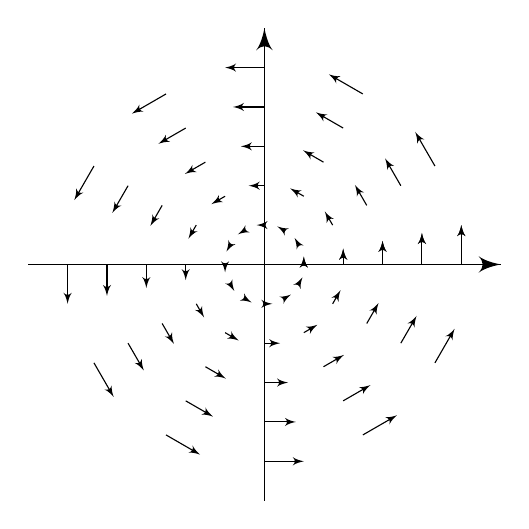
\begin{tikzpicture}
      \draw [->] (-3, 0) -- (3, 0);
      \draw [->] (0, -3) -- (0, 3);

      \foreach \t in {0,30,60,90,120,150,180,210,240,270,300,330,360} {
        \begin{scope}[rotate=\t]
          \draw [-latex'] (2.5, 0) -- +(0, 0.5);
          \draw [-latex'] (2, 0) -- +(0, 0.4);
          \draw [-latex'] (1.5, 0) -- +(0, 0.3);
          \draw [-latex'] (1, 0) -- +(0, 0.2);
          \draw [-latex'] (0.5, 0) -- +(0, 0.1);
        \end{scope}
      }
    \end{tikzpicture}
  \end{center}
  We would expect the integral curves to be circles. Indeed, suppose $\gamma: I \to \R^2$ is an integral curve. Write $\gamma = (\gamma_1, \gamma_2)$. Then the definition requires
  \[
    \gamma_1'(t) \frac{\partial}{\partial x} + \gamma_2'(t) \frac{\partial}{\partial y} = \gamma_1(t) \frac{\partial}{\partial y} - \gamma_2(t) \frac{\partial}{\partial x}.
  \]
  So the equation is
  \begin{align*}
    \gamma_1'(t) &= - \gamma_2(t)\\
    \gamma_2'(t) &= \gamma_1(t).
  \end{align*}
  For example, if our starting point is $p = (1, 0)$, then we have
  \[
    \gamma_1(t) = \cos t,\quad \gamma_2(t) = \sin t.
  \]
\end{eg}
We see that to find an integral curve, all we are doing is just solving ordinary differential equations. We know that all ODEs have smooth and unique solutions, and they have all the nice properties we can hope for. So we are going to get nice corresponding results for integral solutions. However, sometimes funny things happen.

\begin{eg}
  Take $M = \R$, and
  \[
    X = x^2 \frac{\d}{\d x}.
  \]
  Then if $\gamma$ is an integral curve, it must satisfy:
  \[
    \gamma'(t) = \gamma(t)^2.
  \]
  This means that the solution is of the form
  \[
    \gamma(t) = \frac{1}{C - t}
  \]
  for $C$ a constant. For example, if we want $\gamma(0) = \frac{1}{2}$, then we have
  \[
    \gamma(t) = \frac{1}{2 - t}.
  \]
  The solution to this ODE is defined only for $t < 2$, so we can only have $I = (-\infty, 2)$ at best.
\end{eg}

We are going to prove that integral curves always exist. To do so, we need to borrow some powerful theorems from ODE theory:
\begin{thm}[Fundamental theorem on ODEs]
  Let $U \subseteq \R^n$ be open and $\alpha: U \to \R^n$ smooth. Pick $t_0 \in \R$.

  Consider the ODE
  \begin{align*}
    \dot{\gamma}_i(t) &= \alpha_i(\gamma(t))\\
    \gamma_i(t_0) &= c_i,
  \end{align*}
  where $\mathbf{c} = (c_1, \cdots, c_n) \in \R^n$.

  Then there exists an open interval $I$ containing $t_0$ and an open $U_0 \subseteq U$ such that for every $\mathbf{c} \in U_0$, there is a smooth solution $\gamma_\mathbf{c}:I \to U$ satisfying the ODE.

  Moreover, any two solutions agree on a common domain, and the function $\Theta: I \times U_0 \to U$ defined by $\Theta(t, \mathbf{c}) = \gamma_\mathbf{c}(t)$ is smooth (in both variables).
\end{thm}

\begin{thm}[Existence of integral curves]
  Let $X \in \Vect(M)$ and $p \in M$. Then there exists some open interval $I \subseteq \R$ with $0 \in I$ and an integral curve $\gamma: I \to M$ for $X$ with $\gamma(0) = p$.

  Moreover, if $\tilde{\gamma}: \tilde{I} \to M$ is another integral curve for $X$, and $\tilde{\gamma}(0) = p$, then $\tilde{\gamma} = \gamma$ on $I \cap \tilde{I}$.
\end{thm}

\begin{proof}
  Pick local coordinates for $M$ centered at $p$ in an open neighbourhood $U$. So locally we write
  \[
    X = \sum_{i = 1}^n \alpha_i \frac{\partial}{\partial x_i},
  \]
  where $\alpha_i \in C^\infty(U)$. We want to find $\gamma = (\gamma_1, \cdots, \gamma_n): I \to U$ such that
  \[
    \sum_{i = 1}^n \gamma_i'(t) \left.\frac{\partial}{\partial x_i}\right|_{\gamma(t)} = \sum_{i = 1}^n \alpha_i(\gamma(t)) \left.\frac{\partial}{\partial x_i}\right|_{\gamma(t)},\quad \gamma_i(0) = 0.
  \]
  Since the $\frac{\partial}{\partial x_i}$ form a basis, this is equivalent to saying
  \[
    \gamma_i(t) = \alpha_i(\gamma(t)),\quad \gamma_i(0) = 0
  \]
  for all $i$ and $t \in I$.

  By the general theory of ordinary differential equations, there is an interval $I$ and a solution $\gamma$, and any two solutions agree on their common domain.

  However, we need to do a bit more for uniqueness, since all we know is that there is a unique integral curve lying in this particular chart. It might be that there are integral curves that do wild things when they leave the chart.

  So suppose $\gamma: I \to M$ and $\tilde{\gamma}: \tilde{I} \to M$ are both integral curves passing through the same point, i.e.\ $\gamma(0) = \tilde{\gamma}(0) = p$.

  We let
  \[
    J = \{t \in I \cap \tilde{I}: \gamma(t) = \tilde{\gamma}(t)\}.
  \]
  This is non-empty since $0 \in J$, and $J$ is closed since $\gamma$ and $\tilde{\gamma}$ are continuous. To show it is all of $I \cap \tilde{I}$, we only have to show it is open, since $I \cap \tilde{I}$ is connected.

  So let $t_0 \in J$, and consider $q = \gamma(t_0)$. Then $\gamma$ and $\tilde{\gamma}$ are integral curves of $X$ passing through $q$. So by the first part, they agree on some neighbourhood of $t_0$. So $J$ is open. So done.
\end{proof}

\begin{defi}[Maximal integral curve]\index{maximal integral curve}\index{integral curve!maximal}
  Let $p \in M$, and $X \in \Vect(M)$. Let $I_p$ be the union of all $I$ such that there is an integral curve $\gamma: I \to M$ with $\gamma(0) = p$. Then there exists a unique integral curve $\gamma: I_p \to M$, known as the \emph{maximal integral curve}.
\end{defi}

Note that $I_p$ does depend on the point.

\begin{eg}
  Consider the vector field
  \[
    X = \frac{\partial}{\partial x}
  \]
  on $\R^2 \setminus \{0\}$. Then for any point $p = (x, y)$, if $y \not= 0$, we have $I_p = \R$, but if $y = 0$ and $x < 0$, then $I_p = (-\infty, -x)$. Similarly, if $y = 0$ and $x > 0$, then $I_p = (-x, \infty)$.
  \begin{center}
    \begin{tikzpicture}
      \draw (-3, 3) rectangle (3, -3);
      \foreach \x in {-2.7, -1.7, -0.7, 0.3, 1.3, 2.3} {
         \foreach \y in {-2, -1, 0, 1, 2} {
           \draw [-latex'] (\x, \y) -- +(0.4, 0);
         }
      }
      \draw circle [radius=0.1];
    \end{tikzpicture}
  \end{center}
\end{eg}

\begin{defi}[Complete vector field]\index{complete vector field}
  A vector field is \emph{complete} if $I_p = \R$ for all $p \in M$.
\end{defi}

Given a complete vector field, we obtain a flow map as follows:
\begin{thm}\index{$\Theta_t(p)$}
  Let $M$ be a manifold and $X$ a complete vector field on $M$. Define $\Theta_t: \R \times M \to M$ by
  \[
    \Theta_t(p) = \gamma_p(t),
  \]
  where $\gamma_p$ is the maximal integral curve of $X$ through $p$ with $\gamma(0) = p$. Then $\Theta$ is a function smooth in $p$ and $t$, and
  \[
    \Theta_0 = \id,\quad \Theta_t \circ \Theta_s = \Theta_{s + t}
  \]
\end{thm}

\begin{proof}
  This follows from uniqueness of integral curves and smooth dependence on initial conditions of ODEs.
\end{proof}

In particular, since $\Theta_t \circ \Theta_{-t} = \Theta_0 = \id$, we know
\[
  \Theta_t^{-1} = \Theta_{-t}.
\]
So $\Theta_t$ is a diffeomorphism.

More algebraically, if we write $\Diff(M)$ for the diffeomorphisms $M \to M$, then
\begin{align*}
  \R &\to \Diff(M)\\
  t &\mapsto \Theta_t
\end{align*}
is a homomorphism of groups. We call this a \emph{one-parameter subgroup} of diffeomorphisms.

What happens when we relax the completeness assumption? Everything is essentially the same whenever things are defined, but we have to take care of the domains of definition.

\begin{thm}
  Let $M$ be a manifold, and $X \in \Vect(M)$. Define
  \[
    D = \{(t, p) \in \R \times M: t \in I_p\}.
  \]
  In other words, this is the set of all $(t, p)$ such that $\gamma_p(t)$ exists. We set
  \[
    \Theta_t (p) = \Theta(t, p) = \gamma_p(t)
  \]
  for all $(t, p) \in D$. Then
  \begin{enumerate}
    \item $D$ is open and $\Theta: D \to M$ is smooth
    \item $\Theta(0, p) = p$ for all $p \in M$.
    \item If $(t, p) \in D$ and $(t, \Theta(s, p)) \in D$, then $(s + t, p) \in D$ and $\Theta(t, \Theta(s, p)) = \Theta(t + s, p)$.
    \item For any $t \in \R$, the set $M_t: \{p \in M: (t, p) \in D\}$ is open in $M$, and
      \[
        \Theta_t: M_t \to M_{-t}
      \]
      is a diffeomorphism with inverse $\Theta_{-t}$.
  \end{enumerate}
\end{thm}

This is really annoying. We now prove the following useful result that saves us from worrying about these problems in nice cases:
\begin{prop}
  Let $M$ be a compact manifold. Then any $X \in \Vect(M)$ is complete.
\end{prop}

\begin{proof}
  Recall that
  \[
    D = \{(t, p): \Theta_t(p)\text{ is defined}\}
  \]
  is open. So given $p \in M$, there is some open neighbourhood $U \subseteq M$ of $p$ and an $\varepsilon > 0$ such that $(-\varepsilon, \varepsilon) \times U \subseteq D$. By compactness, we can find finitely many such $U$ that cover $M$, and find a small $\varepsilon$ such that $(-\varepsilon, \varepsilon) \times M \subseteq D$.

  In other words, we know $\Theta_t(p)$ exists and $p \in M$ and $|t| < \varepsilon$. Also, we know $\Theta_t \circ \Theta_s = \Theta_{t + s}$ whenever $|t|, |s| < \varepsilon$, and in particular $\Theta_{t + s}$ is defined. So $\Theta_{Nt} = (\Theta_t)^N$ is defined for all $N$ and $|t| < \varepsilon$, so $\Theta_t$ is defined for all $t$.
\end{proof}

\subsection{Lie derivative}
We now want to look at the concept of a Lie derivative. If we have a function $f$ defined on all of $M$, and we have a vector field $X$, then we might want to ask what the derivative of $f$ in the direction of $X$ is at each point. If $f$ is a real-valued function, then this is by definition $X(f)$. If $f$ is more complicated, then this wouldn't work, but we can still differentiate things along $X$ using the flows.

\begin{notation}\index{$F^*g$}
  Let $F: M \to M$ be a diffeomorphism, and $g \in C^\infty(M)$. We write
  \[
    F^* g = g \circ F \in C^\infty(M).
\]
\end{notation}

We now define the \emph{Lie derivative} of a function, i.e.\ the derivative of a function $f$ in the direction of a vector field $X$. Of course, we can obtain this by just applying $X(f)$, but we want to make a definition that we can generalize.

\begin{defi}[Lie derivative of a function]\index{Lie derivative!function}
  Let $X$ be a complete vector field, and $\Theta$ be its flow. We define the \emph{Lie derivative} of $g$ along $X$ by
  \[
    \mathcal{L}_X(g) = \left.\frac{\d}{\d t} \right|_{t = 0} \Theta_t^* g.
  \]
  Here this is defined pointwise, i.e.\ for all $p \in M$, we define
  \[
    \mathcal{L}_X(g)(p) = \left.\frac{\d}{\d t}\right|_{t = 0} \Theta_t^*(g)(p).
  \]
\end{defi}

\begin{lemma}
  $\mathcal{L}_X(g) = X(g)$. In particular, $\mathcal{L}_X(g) \in C^\infty(M, \R)$.
\end{lemma}

\begin{proof}
  \begin{align*}
    \mathcal{L}_X(g)(p) &= \left.\frac{\d}{\d t}\right|_{t = 0} \Theta_t^*(g)(p) \\
    &= \left.\frac{\d}{\d t}\right|_{t = 0} g(\Theta_t(p)) \\
    &= \d g|_p(X(p))\\
    &= X(g)(p). \qedhere
  \end{align*}
\end{proof}

So this is quite boring. However, we can do something more exciting by differentiating vector fields.

\begin{notation}\index{$F^*(Y)$}
  Let $Y \in \Vect(M)$, and $F: M \to M$ be a diffeomorphism. Then $\D F^{-1}|_{F(p)}: T_{F(p)} M \to T_pM$. So we can write
  \[
    F^*(Y)|_p = \D F^{-1}|_{F(p)}(Y_{F(p)}) \in T_p M.
  \]
  Then $F^*(Y) \in \Vect(M)$. If $g \in C^\infty(M)$, then
  \[
    F^*(Y)|_p(g) = Y_{F(p)} (g \circ F^{-1}).
  \]
  Alternatively, we have
  \[
    F^*(Y)|_p(g \circ F) = Y_{F(p)}(g).
  \]
  Removing the $p$'s, we have
  \[
    F^*(Y)(g \circ F) = (Y(g)) \circ F.
  \]
\end{notation}

\begin{defi}[Lie derivative of a vector field]\index{Lie derivative!vector field}
  Let $X \in \Vect(M)$ be complete, and $Y \in \Vect(M)$ be a vector field. Then the \emph{Lie derivative} is given pointwise by
  \[
    \mathcal{L}_X(Y) = \left.\frac{\d}{\d t}\right|_{t = 0} \Theta_t^*(Y).
  \]
\end{defi}

\begin{lemma}
  We have
  \[
    \mathcal{L}_X Y = [X, Y].
  \]
\end{lemma}

\begin{proof}
  Let $g \in C^\infty(M, \R)$. Then we have
  \[
    \Theta_t^*(Y)(g \circ \Theta_t) = Y(g) \circ \Theta_t.
  \]
  We now look at
  \[
    \frac{\Theta_t^* (Y)(g) - Y(g)}{t} = \underbrace{\frac{\Theta_t^*(Y)(g) - \Theta_t^*(Y)(g \circ \Theta_t)}{t}}_{\alpha_t} + \underbrace{\frac{Y(g) \circ \Theta_t - Y(g)}{t}}_{\beta_t}.
  \]
  We have
  \[
    \lim_{t \to 0} \beta_t = \mathcal{L}_X (Y(g)) = XY(g)
  \]
  by the previous lemma, and we have
  \[
    \lim_{t\to 0}\alpha_t = \lim_{t \to 0} (\Theta_t^*(Y))\left(\frac{g - g \circ \Theta_t}{t}\right) = Y(-\mathcal{L}_X(g)) = - YX(g). \qedhere
  \]
\end{proof}

\begin{cor}
  Let $X, Y \in \Vect(M)$ and $f \in C^\infty(M, \R)$. Then
  \begin{enumerate}
    \item $\mathcal{L}_X(fY) = \mathcal{L}_X(f) Y + f \mathcal{L}_X Y = X(f) Y + f \mathcal{L}_X Y$
    \item $\mathcal{L}_X Y = - \mathcal{L}_Y X$
    \item $\mathcal{L}_X[Y, Z] = [\mathcal{L}_X Y, Z] + [Y, \mathcal{L}_X Z]$.
  \end{enumerate}
\end{cor}

\begin{proof}
  Immediate from the properties of the Lie bracket.
\end{proof}

\section{Lie groups}
We now have a short digression to Lie groups. Lie groups are manifolds with a group structure. They have an extraordinary amount of symmetry, since multiplication with any element of the group induces a diffeomorphism of the Lie group, and this action of the Lie group on itself is free and transitive. Effectively, this means that any two points on the Lie group, as a manifold, are ``the same''.

As a consequence, a lot of the study of a Lie group reduces to studying an infinitesimal neighbourhood of the identity, which in turn tells us about infinitesimal neighbourhoods of \emph{all points} on the manifold. This is known as the \emph{Lie algebra}.

We are not going to go deep into the theory of Lie groups, as our main focus is on differential geometry. However, we will state a few key results about Lie groups.

\begin{defi}[Lie group]\index{Lie group}
  A \emph{Lie group} is a manifold $G$ with a group structure such that multiplication $m: G \times G \to G$ and inverse $i: G \to G$ are smooth maps.
\end{defi}

%\begin{own}
%  \begin{defi}[Lie group]
%    A \emph{Lie group} is a group object in the category of smooth manifolds.
%  \end{defi}
%\end{own}

\begin{eg}
  $\GL_n(\R)$ and $\GL_n(\C)$ are Lie groups.
\end{eg}

\begin{eg}
  $M_n(\R)$ under addition is also a Lie group.
\end{eg}

\begin{eg}
  $\Or(n)$ is a Lie group.
\end{eg}

\begin{notation}\index{$L_g$}
  Let $G$ be a Lie group and $g \in G$. We write $L_g: G \to G$ for the diffeomorphism
  \[
    L_g(h) = gh.
  \]
\end{notation}
This innocent-seeming translation map is what makes Lie groups nice. Given any local information near an element $g$, we can transfer it to local information near $h$ by applying the diffeomorphism $L_{hg^{-1}}$. In particular, the diffeomorphism $L_g: G \to G$ induces a linear isomorphism $\D L_g|_e : T_e G \to T_g G$, so we have a canonical identification of all tangent spaces.

\begin{defi}[Left invariant vector field]\index{left invariant vector field}\index{vector field!left invariant}
  Let $X \in \Vect(G)$ be a vector field. This is \emph{left invariant} if
  \[
    \D L_g|_h (X_h) = X_{gh}
  \]
  for all $g,h \in G$.

  We write $\Vect^L(G)$\index{$\Vect^L(G)$} for the collection of all left invariant vector fields.
\end{defi}

Using the fact that for a diffeomorphism $F$, we have
\[
  F^*[X, Y] = [F^* X, F^* Y],
\]
it follows that $\Vect^L(G)$ is a Lie subalgebra of $\Vect(G)$.

If we have a left invariant vector field, then we obtain a tangent vector at the identity. On the other hand, if we have a tangent vector at the identity, the definition of a left invariant vector field tells us how we can extend this to a left invariant vector field. One would expect this to give us an isomorphism between $T_e G$ and $\Vect^L(G)$, but we have to be slightly more careful and check that the induced vector field is indeed a vector field.

\begin{lemma}
  Given $\xi \in T_e G$, we let
  \[
    X_\xi|_g = \D L_g|_e(\xi) \in T_g(G).
  \]
  Then the map $T_e G \to \Vect^L(G)$ by $\xi \mapsto X_\xi$ is an isomorphism of vector spaces.
\end{lemma}

\begin{proof}
  The inverse is given by $X \mapsto X|_e$. The only thing to check is that $X_\xi$ actually is a left invariant vector field. The left invariant part follows from
  \[
    \D L_h|_g (X_\xi|_g) = \D L_h|_g (\D L_g|_e (\xi)) = \D L_{hg}|_e(\xi) = X_\xi |_{hg}.
  \]
  To check that $X_\xi$ is smooth, suppose $f \in C^\infty(U, \R)$, where $U$ is open and contains $e$. We let $\gamma: (-\varepsilon, \varepsilon) \to U$ be smooth with $\dot{\gamma}(0) = \xi$. So
  \[
    X_\xi f|_g = \D L_g (\xi)(f) = \xi(f \circ L_g) = \left.\frac{\d}{\d t}\right|_{t = 0} (f \circ L_g \circ \gamma)
  \]
  But as $(t, g) \mapsto f \circ L_g \circ \gamma(t)$ is smooth, it follows that $X_\xi f$ is smooth. So $X_\xi \in \Vect^L(G)$.
\end{proof}

Thus, instead of talking about $\Vect^L(G)$, we talk about $T_e G$, because it seems less scary. This isomorphism gives $T_eG$ the structure of a Lie algebra.

\begin{defi}[Lie algebra of a Lie group]\index{Lie algebra of Lie group}
  Let $G$ be a Lie group. The \emph{Lie algebra} $\mathfrak{g}$ of $G$ is the Lie algebra $T_eG$ whose Lie bracket is induced by that of the isomorphism with $\Vect^L(G)$. So
  \[
    [\xi, \eta] = [X_\xi, X_\eta]|_e.
  \]
  We also write $\Lie(G)$ for $\mathfrak{g}$.
\end{defi}
In general, if a Lie group is written in some capital letter, say $G$, then the Lie algebra is written in the same letter but in lower case fraktur.

Note that $\dim \mathfrak{g} = \dim G$ is finite.

\begin{lemma}
  Let $G$ be an abelian Lie group. Then the bracket of $\mathfrak{g}$ vanishes.
\end{lemma}

\begin{eg}
  For any vector space $V$ and $v \in V$, we have $T_v V \cong V$. So $V$ as a Lie group has Lie algebra $V$ itself. The commutator vanishes because the group is commutative.
\end{eg}

\begin{eg}
  Note that $G = \GL_n(\R)$ is an open subset of $M_n$, so it is a manifold. It is then a Lie group under multiplication. Then we have
  \[
    \gl_n(\R) = \Lie(\GL_n(\R)) = T_I \GL_n(\R) = T_I M_n \cong M_n.
  \]
  If $A, B \in \GL_n(\R)$, then
  \[
    L_A(B) = AB.
  \]
  So
  \[
    \D L_A|_B(H) = AH
  \]
  as $L_A$ is linear.

  We claim that under the identification, if $\xi, \eta \in \gl_n(\R) = M_n$, then
  \[
    [\xi, \eta] = \xi \eta - \eta \xi.
  \]
  Indeed, on $G$, we have global coordinates $U_i^j: \GL_n(\R) \to \R$ where
  \[
    U_i^j(A) = A_i^j,
  \]
  where $A = (A_i^j) \in \GL_n(\R)$.

  Under this chart, we have
  \[
    X_\xi|_A = L_A(\xi) = \sum_{i,j} (A \xi)_j^i \left.\frac{\partial}{\partial U_j^i}\right|_A = \sum_{i,j,k} A_k^i \xi_j^k \left.\frac{\partial}{\partial U_j^i} \right|_A
  \]
  So we have
  \[
    X_\xi = \sum_{i,j,k} U^i_k \xi^k_j \frac{\partial}{\partial U_j^i}.
  \]
  So we have
  \[
    [X_\xi, X_\eta] = \left[\sum_{i,j,k} U_k^i \xi_j^k \frac{\partial}{\partial U_j^i},\sum_{p, r, q} U_q^p \eta_r^q \frac{\partial}{\partial U_r^p}\right].
  \]
  We now use the fact that
  \[
    \frac{\partial}{\partial U^i_j} U^p_q = \delta_{ip}\delta_{jq}.
  \]
  We then expand
  \[
    [X_\xi, X_\eta] = \sum_{i,j,k,r} (U_j^i \xi_k^j \eta^k_r - U^i_j \xi^j_k \xi^k_r) \frac{\partial}{\partial U_r^i}.
  \]
  So we have
  \[
    [X_\xi, X_\eta] = X_{\xi\eta - \eta\xi}.
  \]
\end{eg}

\begin{defi}[Lie group homomorphisms]\index{Lie group!homomorphism}
  Let $G, H$ be Lie groups. A \emph{Lie group homomorphism} is a smooth map that is also a homomorphism.
\end{defi}

\begin{defi}[Lie algebra homomorphism]\index{Lie algebra!homomorphism}
  Let $\mathfrak{g}, \mathfrak{h}$ be Lie algebras. Then a \emph{Lie algebra homomorphism} is a linear map $\beta: \mathfrak{g} \to \mathfrak{h}$ such that
  \[
    \beta[\xi,\eta] = [\beta(\xi), \beta(\eta)]
  \]
  for all $\xi,\eta \in \mathfrak{g}$.
\end{defi}

\begin{prop}
  Let $G$ be a Lie group and $\xi \in \mathfrak{g}$. Then the integral curve $\gamma$ for $X_\xi$ through $e \in G$ exists for all time, and $\gamma: \R \to G$ is a Lie group homomorphism.
\end{prop}

The idea is that once we have a small integral curve, we can use the Lie group structure to copy the curve to patch together a long integral curve.
\begin{proof}
  Let $\gamma: I \to G$ be a maximal integral curve of $X_\xi$, say $(-\varepsilon, \varepsilon) \in I$. We fix a $t_0$ with $|t_0| < \varepsilon$. Consider $g_0 = \gamma(t_0)$.

  We let
  \[
    \tilde{\gamma}(t) = L_{g_0}(\gamma(t))
  \]
  for $|t| < \varepsilon$.

  We claim that $\tilde{\gamma}$ is an integral curve of $X_\xi$ with $\tilde{\gamma}(0) = g_0$. Indeed, we have
  \[
    \dot{\tilde{\gamma}}|_t = \frac{\d}{\d t} L_{g_0}\gamma(t) = \D L_{g_0} \dot{\gamma}(t) = \D L_{g_0} X_\xi|_{\gamma(t)} = X_\xi|_{g_0 \cdot \gamma(t)} = X_\xi|_{\tilde{\gamma}(t)}.
  \]
  By patching these together, we know $(t_0 - \varepsilon, t_0 + \varepsilon) \subseteq I$. Since we have a fixed $\varepsilon$ that works for all $t_0$, it follows that $I = \R$.

  The fact that this is a Lie group homomorphism follows from general properties of flow maps.
\end{proof}

\begin{eg}
  Let $G = \GL_n$. If $\xi \in \gl_n$, we set
  \[
    e^\xi = \sum_{k \geq 0} \frac{1}{k!} \xi^k.
  \]
  We set $F(t) = e^{t \xi}$. We observe that this is in $\GL_n$ since $e^{t\xi}$ has an inverse $e^{-t\xi}$ (alternatively, $\det (e^{t\xi}) = e^{\tr (t\xi)} \not= 0$). Then
  \[
    F'(t) = \frac{\d}{\d t} \sum_k \frac{1}{k!} t^k \xi^k = e^{t\xi} \xi = L_{e^{t\xi}}\xi = L_{F(t)}\xi.
  \]
  Also, $F(0) = I$. So $F(t)$ is an integral curve.
\end{eg}

\begin{defi}[Exponential map]\index{exponential map}
  The \emph{exponential map} of a Lie group $G$ is $\exp: \mathfrak{g} \to G$ given by
  \[
    \exp(\xi) = \gamma_\xi(1),
  \]
  where $\gamma_\xi$ is the integral curve of $X_\xi$ through $e \in G$.
\end{defi}
So in the case of $G = \GL_n$, the exponential map is the exponential map.

\begin{prop}\leavevmode
  \begin{enumerate}
    \item $\exp$ is a smooth map.
    \item If $F(t) = \exp(t\xi)$, then $F: \R \to G$ is a Lie group homomorphism and $\D F|_0 \left(\frac{\d}{\d t}\right) = \xi$.
    \item The derivative
      \[
        \D \exp: T_0 \mathfrak{g} \cong \mathfrak{g} \to T_e G \cong \mathfrak{g}
      \]
      is the identity map.
    \item $\exp$ is a local diffeomorphism around $0 \in \mathfrak{g}$, i.e.\ there exists an open $U \subseteq \mathfrak{g}$ containing $0$ such that $\exp: U \to \exp(U)$ is a diffeomorphism.
    \item $\exp$ is natural, i.e.\ if $f: G \to H$ is a Lie group homomorphism, then the diagram
      \[
        \begin{tikzcd}
          \mathfrak{g} \ar[r, "\exp"] \ar[d, "\D f|_e"]& G \ar[d, "f"]\\
          \mathfrak{h} \ar[r, "\exp"] & H
        \end{tikzcd}
      \]
      commutes.
  \end{enumerate}
\end{prop}

\begin{proof}\leavevmode
  \begin{enumerate}
    \item This is the smoothness of ODEs with respect to parameters
    \item Exercise.
    \item If $\xi \in \mathfrak{g}$, we let $\sigma(t) = t \xi$. So $\dot{\sigma}(0) = \xi \in T_0 \mathfrak{g} \cong \mathfrak{g}$. So
      \[
        \D \exp|_0 (\xi) = \D \exp|_0(\dot{\sigma}(0)) = \left.\frac{\d}{\d t}\right|_{t = 0} \exp(\sigma(t)) = \left.\frac{\d}{\d t}\right|_{t = 0} \exp(t \xi) = X_\xi|_e = \xi.
      \]
    \item Follows from above by inverse function theorem.
    \item Exercise. \qedhere
  \end{enumerate}
\end{proof}

\begin{defi}[Lie subgroup]\index{Lie subgroup}\index{Lie group!subgroup}
  A \emph{Lie subgroup} of $G$ is a subgroup $H$ with a smooth structure on $H$ making $H$ an \emph{immersed} submanifold.
\end{defi}

Certainly, if $H \subseteq G$ is a Lie subgroup, then $\mathfrak{h} \subseteq \mathfrak{g}$ is a Lie subalgebra.

\begin{thm}
  If $\mathfrak{h} \subseteq \mathfrak{g}$ is a subalgebra, then there exists a unique connected Lie subgroup $H \subseteq G$ such that $\Lie(H) = \mathfrak{h}$.
\end{thm}

\begin{thm}
  Let $\mathfrak{g}$ be a finite-dimensional Lie algebra. Then there exists a (unique) simply-connected Lie group $G$ with Lie algebra $\mathfrak{g}$.
\end{thm}

\begin{thm}
  Let $G, H$ be Lie groups with $G$ simply connected. Then every Lie algebra homomorphism $\mathfrak{g} \to \mathfrak{h}$ lifts to a Lie group homomorphism $G \to H$.
\end{thm}

\section{Vector bundles}
Recall that we had the tangent bundle of a manifold. The tangent bundle gives us a vector space at each point in space, namely the tangent space. In general, a vector bundle is a vector space attached to each point in our manifold (in a smoothly-varying way), which is what we are going to study in this chapter.

Before we start, we have a look at tensor products. These will provide us a way of constructing new vector spaces from old ones.

\subsection{Tensors} % Return to this
The tensor product is a very important concept in Linear Algebra. It is something that is taught in no undergraduate courses and assumed knowledge in all graduate courses. For the benefit of the students, we will give a brief introduction to tensor products.

A motivation for tensors comes from the study of bilinear maps. A bilinear map is a function that takes in two vectors and returns a number, and this is linear in both variables. An example is the inner product, and another example is the volume form, which tells us the volume of a parallelepiped spanned by the two vectors.

\begin{defi}[Bilinear map]\index{bilinear map}
  Let $U, V, W$ be vector spaces. We define $\Bilin(V\times W, U)$ to be the functions $V \times W \to U$ that are bilinear, i.e.\
  \begin{align*}
    \alpha(\lambda_1 v_1 + \lambda_2 v_2, w) &= \lambda_1 \alpha(v_1, w) + \lambda_2 \alpha(v_2, w)\\
    \alpha(v, \lambda_1 w_1 + \lambda_2 w_2) &= \lambda_1 \alpha(v, w_1) + \lambda_2 \alpha(v, w_2).
  \end{align*}
\end{defi}
It is important that a bilinear map is not a linear map. This is bad. We spent so much time studying linear maps, and we now have to go back to our linear algebra book and rewrite everything to talk about bilinear maps as well. But bilinear maps are not enough. We want to do them for multi-linear maps! But linear maps were already complicated enough, so this must be much worse. We want to die.

Tensors are a trick to turn the study of bilinear maps to linear maps (from a different space).

\begin{defi}[Tensor product]\index{tensor product}
  A \emph{tensor product} of two vector spaces $V, W$ is a vector space $V \otimes W$ and a bilinear map $\pi: V \times W \to V \otimes W$ such that a bilinear map from $V \times W$ is ``the same as'' a linear map from $V \otimes W$. More precisely, given any bilinear map $\alpha: V \times W \to U$, we can find a unique linear map $\tilde{\alpha}: V \otimes W \to U$ such that the following diagram commutes:
  \[
    \begin{tikzcd}
      V \times W \ar[rd, "\alpha"] \ar[d, "\pi"] \\
      V \otimes W \ar[r, "\tilde\alpha"'] & U
    \end{tikzcd}
  \]
  So we have
  \[
    \Bilin(V \times W, U) \cong \Hom(V \otimes W, U).
  \]
  Given $v \in V$ and $w \in W$, we obtain $\pi(v, w) \in V \otimes W$, called the \emph{tensor product} of $v$ and $w$, written $v \otimes w$.
\end{defi}
We say $V \otimes W$ \emph{represents} bilinear maps from $V \times W$.

It is important to note that not all elements of $V \otimes W$ are of the form $v \otimes w$.

Now the key thing we want to prove is the \emph{existence} and uniqueness of tensor products.

\begin{lemma}
  Tensor products exist (and are unique up to isomorphism) for all pairs of finite-dimensional vector spaces.
\end{lemma}

\begin{proof}
  We can construct $V \otimes W = \Bilin(V \times W, \R)^*$. The verification is left as an exercise on the example sheet.
\end{proof}

We now write down some basic properties of tensor products.
\begin{prop}
  Given maps $f: V \to W$ and $g: V' \to W'$, we obtain a map $f \otimes g: V \otimes V' \to W \otimes W'$ given by the bilinear map
  \[
    (f \otimes g)(v, w) = f(v) \otimes g(w).
  \]
\end{prop}

\begin{lemma}
  Given $v, v_i \in V$ and $w, w_i \in W$ and $\lambda_i \in \R$, we have
  \begin{align*}
    (\lambda_1 v_1 + \lambda_2 v_2) \otimes w &= \lambda_1 (v_1 \otimes w) + \lambda_2 (v_2 \otimes w)\\
    v \otimes (\lambda_1 w_1 + \lambda_2 w_2) &= \lambda_1 (v \otimes w_1) + \lambda_2 (v \otimes w_2).
  \end{align*}
\end{lemma}

\begin{proof}
  Immediate from the definition of bilinear map.
\end{proof}

\begin{lemma}
  If $v_1,\cdots, v_n$ is a basis for $V$, and $w_1, \cdots, w_m$ is a basis for $W$, then
  \[
    \{v_i \otimes w_j: i = 1, \cdots, n; j = 1, \cdots, m\}
  \]
  is a basis for $V \otimes W$. In particular, $\dim V \otimes W = \dim V \times \dim W$.
\end{lemma}

\begin{proof}
  We have $V \otimes W = \Bilin(V \times W, \R)^*$. We let $\alpha_{pq}:V \times W \to \R$ be given by
  \[
    \alpha_{pq}\left(\sum a_i v_i, \sum b_j w_j\right) = a_p b_q.
  \]
  Then $\alpha_{pq} \in \Bilin(V\times W, \R)$, and $(v_i \otimes w_j)$ are dual to $\alpha_{pq}$. So it suffices to show that $\alpha_{pq}$ are a basis. It is clear that they are independent, and any bilinear map can be written as
  \[
    \alpha = \sum c_{pq}\alpha_{pq},
  \]
  where
  \[
    c_{pq} = \alpha(v_p, w_q).
  \]
  So done.
\end{proof}

\begin{prop}
  For any vector spaces $V, W, U$, we have (natural) isomorphisms
  \begin{enumerate}
    \item $V \otimes W \cong W \otimes V$
    \item $(V \otimes W) \otimes U \cong V \otimes (W \otimes U)$
    \item $(V \otimes W)^* \cong V^* \otimes W^*$
  \end{enumerate}
\end{prop}

\begin{defi}[Covariant tensor]\index{covariant tensor}
  A \emph{covariant tensor} of rank $k$ on $V$ is an element of
  \[
    \alpha \in \underbrace{V^* \otimes \cdots \otimes V^*}_{k\text{ times}},
  \]
  i.e.\ $\alpha$ is a multilinear map $V \times \cdots \times V \to \R$.
\end{defi}

\begin{eg}
  A covariant $1$-tensor is an $\alpha \in V^*$, i.e.\ a linear map $\alpha: V \to \R$.

  A covariant $2$-tensor is a $\beta \in V^* \otimes V^*$, i.e.\ a bilinear map $V \times V \to \R$, e.g.\ an inner product.
\end{eg}

\begin{eg}
  If $\alpha, \beta \in V^*$, then $\alpha \otimes \beta \in V^* \otimes V^*$ is the covariant $2$-tensor given by
  \[
    (\alpha \otimes b)(v, w) = \alpha(v) \beta(w).
  \]
  More generally, if $\alpha$ is a rank $k$ tensor and $\beta$ is a rank $\ell$ tensor, then $\alpha \otimes \beta$ is a rank $k + \ell$ tensor.
\end{eg}

\begin{defi}[Tensor]\index{tensor}
  A \emph{tensor} of type $(k, \ell)$ is an element in
  \[
    T^k_\ell(V) = \underbrace{V^* \otimes \cdots \otimes V^*}_{k\text{ times}} \otimes \underbrace{V \otimes \cdots \otimes V}_{\ell\text{ times}}.
  \]
\end{defi}
We are interested in alternating bilinear maps, i.e.\ $\alpha(v, w) = - \alpha(w, v)$, or equivalently, $\alpha(v, v) = 0$ (if the characteristic is not $2$).

\begin{defi}[Exterior product]\index{exterior product}\index{exterior algebra}
  Consider
  \[
    T(V) = \bigoplus_{k \geq 0} V^{\otimes k}
  \]
  as an algebra (with multiplication given by the tensor product) (with $V^{\otimes 0} = \R$). We let $I(V)$ be the ideal (as algebras!) generated by $\{v \otimes v: v \in V\} \subseteq T(V)$. We define
  \[
    \Lambda (V) = T(V)/I(V),
  \]
  with a projection map $\pi: T(V) \to \Lambda(V)$. This is known as the \emph{exterior algebra}. We let
  \[
    \Lambda^k(V) = \pi(V^{\otimes k}),
  \]
  the \emph{$k$-th exterior product} of $V$.

  We write $a \wedge b$ for $\pi(\alpha \otimes \beta)$.
\end{defi}

The idea is that $\Lambda^p V$ is the dual of the space of alternating multilinear maps $V \times V\to \R$.

\begin{lemma}\leavevmode
  \begin{enumerate}
    \item If $\alpha \in \Lambda^p V$ and $\beta \in \Lambda^q V$, then $\alpha \wedge \beta = (-1)^{pq} \beta \wedge \alpha$.
    \item If $\dim V = n$ and $p > n$, then we have
      \[
        \dim \Lambda^0 V = 1,\quad \dim \Lambda^n V = 1,\quad \Lambda^p V = \{0\}.
      \]
    \item The multilinear map $\det: V \times \cdots \times V \to \R$ spans $\Lambda^n V$.
    \item If $v_1, \cdots, v_n$ is a basis for $V$, then
      \[
        \{v_{i_1} \wedge \cdots \wedge v_{i_p}: i_1 < \cdots < i_p\}
      \]
      is a basis for $\Lambda^p V$.
  \end{enumerate}
\end{lemma}

\begin{proof}\leavevmode
  \begin{enumerate}
    \item We clearly have $v \wedge v = 0$. So
      \[
        v \wedge w = - w \wedge v
      \]
      Then
      \[
        (v_1 \wedge \cdots \wedge v_p) \wedge (w_1 \wedge \cdots \wedge w_q) = (-1)^{pq} w_1 \wedge \cdots \wedge w_q \wedge v_1 \wedge \cdots \wedge v_p
      \]
      since we have $pq$ swaps. Since
      \[
        \{v_{i_1} \wedge \cdots \wedge v_{i_p}: i_1, \cdots, i_p \in \{1,\cdots, n\}\} \subseteq \Lambda^p V
      \]
      spans $\Lambda^p V$ (by the corresponding result for tensor products), the result follows from linearity.
    \item Exercise.
    \item The $\det$ map is non-zero. So it follows from the above.
    \item We know that
      \[
        \{v_{i_1} \wedge \cdots \wedge v_{i_p}: i_1, \cdots, i_p \in \{1,\cdots, n\}\} \subseteq \Lambda^p V
      \]
      spans, but they are not independent since there is a lot of redundancy (e.g.\ $v_1 \wedge v_2 = - v_2 \wedge v_1$). By requiring $i_1 < \cdots < i_p$, then we obtain a unique copy for combination.

      To check independence, we write $I = (i_1, \cdots, i_p)$ and let $v_I = v_{i_1} \wedge \cdots \wedge v_{i_p}$. Then suppose
      \[
        \sum_I a_I v_I = 0
      \]
      for $a_I \in \R$. For each $I$, we let $J$ be the multi-index $J = \{1, \cdots, n\} \setminus I$. So if $I \not= I'$, then $v_{I'} \wedge v_J = 0$. So wedging with $v_J$ gives
      \[
        \sum_{I'} \alpha_{I'} v_{I'} \wedge v_J = a_I v_I \wedge v_J = 0.
      \]
      So $a_I = 0$. So done by (ii). \qedhere
  \end{enumerate}
\end{proof}

If $F: V \to W$ is a linear map, then we get an induced linear map $\Lambda^p F: \Lambda^p V \to \Lambda^p W$ in the obvious way, making the following diagram commute:
\[
  \begin{tikzcd}
    V^{\otimes p} \ar[r, "F^{\otimes p}"] \ar[d, "\pi"] & W^{\otimes p} \ar[d, "\pi"]\\
    \Lambda^p V \ar[r, "\Lambda^p F"] & \Lambda^p W
  \end{tikzcd}
\]
More concretely, we have
\[
  \Lambda^p F (v_1 \wedge \cdots \wedge v_p) = F(v_1) \wedge \cdots \wedge F(v_p).
\]
\begin{lemma}
  Let $F: V \to V$ be a linear map. Then $\Lambda^n F: \Lambda^n V \to \Lambda^n V$ is multiplication by $\det F$.
\end{lemma}

\begin{proof}
  Let $v_1, \cdots, v_n$ be a basis. Then $\Lambda^n V$ is spanned by $v_1 \wedge \cdots \wedge v_n$. So we have
  \[
    (\Lambda^n F)(v_1\wedge \cdots \wedge v_n) = \lambda \, v_1 \wedge \cdots \wedge v_n
  \]
  for some $\lambda$. Write
  \[
    F(v_i) = \sum_j A_{ji} v_j
  \]
  for some $A_{ji} \in \R$, i.e.\ $A$ is the matrix representation of $F$. Then we have
  \[
    (\Lambda^n F)(v_1 \wedge \cdots \wedge v_n) = \biggl(\sum_j A_{j1} v_j\biggr) \wedge \cdots \wedge \biggl(\sum_j A_{jn} v_j\biggr).
  \]
  If we expand the thing on the right, a lot of things die. The only things that live are those where we get each of $v_i$ once in the wedges in some order. Then this becomes
  \[
    \sum_{\sigma \in S_n} \varepsilon(\sigma) (A_{\sigma(1), 1} \cdots A_{\sigma(n), n}) v_1 \wedge \cdots \wedge v_n = \det(F) \, v_1 \wedge \cdots \wedge v_n,
  \]
  where $\varepsilon(\sigma)$ is the sign of the permutation, which comes from rearranging the $v_i$ to the right order.
\end{proof}

\subsection{Vector bundles}
Our aim is to consider spaces $T_p M \otimes T_p M, \ldots, \Lambda^r T_p M$ etc as $p$ varies, i.e.\ construct a ``tensor bundle'' for these tensor products, similar to how we constructed the tangent bundle. Thus, we need to come up with a general notion of vector bundle.

\begin{defi}[Vector bundle]\index{vector bundle}
  A \emph{vector bundle} of rank $r$ on $M$ is a smooth manifold $E$ with a smooth $\pi: E \to M$ such that
  \begin{enumerate}
    \item For each $p \in M$, the fiber $\pi^{-1}(p) = E_p$ is an $r$-dimensional vector space,
    \item For all $p \in M$, there is an open $U \subseteq M$ containing $p$ and a diffeomorphism
      \[
        t: E|_U = \pi^{-1}(U) \to U \times \R^r
      \]
      such that
      \[
        \begin{tikzcd}
          E|_U \ar[r, "t"] \ar[d, "\pi"] & U \times \R^r \ar[dl, "p_1"]\\
          U
        \end{tikzcd}
      \]
      commutes, and the induced map $E_q \to \{q\} \times \R^r$ is a linear isomorphism for all $q \in U$.

      We call $t$ a \term{trivialization} of $E$ over $U$; call $E$ the \term{total space}; call $M$ the \term{base space}; and call $\pi$ the \term{projection}. Also, for each $q \in M$, the vector space $E_q = \pi^{-1}(\{q\})$ is called the \term{fiber} over $q$.
  \end{enumerate}
  Note that the vector space structure on $E_p$ is part of the data of a vector bundle.
\end{defi}

Alternatively, $t$ can be given by collections of smooth maps $s_1, \cdots, s_r: U \to E$ with the property that for each $q \in U$, the vectors $s_1(q), \cdots, s_r(q)$ form a basis for $E_q$. Indeed, given such $s_1, \cdots, s_r$, we can define $t$ by
\[
  t(v_q) = (q, \alpha_1, \cdots, \alpha_r),
\]
where $v_q \in E_q$ and the $\alpha_i$ are chosen such that
\[
  v_q = \sum_{i = 1}^r \alpha_i s_i(q).
\]
The $s_1, \cdots, s_r$ are known as a \term{frame} for $E$ over $U$.

\begin{eg}[Tangent bundle]
  The bundle $TM \to M$ is a vector bundle. Given any point $p$, find some coordinate charts around $p$ with coordinates $x_1, \cdots, x_n$. Then we get a frame $\frac{\partial}{\partial x_i}$, giving trivializations of $TM$ over $U$. So $TM$ is a vector bundle.
\end{eg}

\begin{defi}[Section]\index{section}\index{$C^\infty(U, E)$}
  A \emph{(smooth) section} of a vector bundle $E \to M$ over some open $U \subseteq M$ is a smooth $s: U \to E$ such that $s(p) \in E_p$ for all $p \in U$, that is $\pi \circ s = \id$. We write $C^\infty(U, E)$ for the set of smooth sections of $E$ over $U$.
\end{defi}

\begin{eg}
  $\Vect(M) = C^\infty (M, TM)$.
\end{eg}

\begin{defi}[Transition function]\index{transition function}
  Suppose that $t_\alpha: E|_{U_\alpha} \to U_\alpha \times \R^r$ and $t_\beta: E|_{U_\beta} \to U_\beta \times \R^r$ are trivializations of $E$. Then
  \[
    t_\alpha \circ t_\beta^{-1} : (U_\alpha \cap U_\beta) \times \R^r \to (U_\alpha \cap U_\beta) \times \R^r
  \]
  is fiberwise linear, i.e.
  \[
    t_\alpha \circ t_\beta^{-1}(q, v) = (q, \varphi_{\alpha\beta}(q) v),
  \]
  where $\varphi_{\alpha\beta}(q)$ is in $\GL_r(\R)$.

  In fact, $\varphi_{\alpha\beta}: U_\alpha \cap U_\beta \to \GL_r(\R)$ is smooth. Then $\varphi_{\alpha\beta}$ is known as the \term{transition function} from $\beta$ to $\alpha$.
\end{defi}

\begin{prop}
  We have the following equalities whenever everything is defined:
  \begin{enumerate}
    \item $\varphi_{\alpha\alpha} = \id$
    \item $\varphi_{\alpha\beta} = \varphi_{\beta\alpha}^{-1}$
    \item $\varphi_{\alpha\beta}\varphi_{\beta\gamma} = \varphi_{\alpha\gamma}$, where $\varphi_{\alpha\beta} \varphi_{\beta\gamma}$ is pointwise matrix multiplication.
  \end{enumerate}
  These are known as the \term{cocycle conditions}.
\end{prop}
We now consider general constructions that allow us to construct new vector bundles from old ones.

\begin{prop}[Vector bundle construction]
  Suppose that for each $p \in M$, we have a vector space $E_p$. We set
  \[
    E = \bigcup_p E_p
  \]
  We let $\pi: E \to M$ be given by $\pi(v_p) = p$ for $v_p \in E_p$. Suppose there is an open cover $\{U_\alpha\}$ of open sets of $M$ such that for each $\alpha$, we have maps
  \[
    t_\alpha: E|_{U_\alpha} = \pi^{-1}(U_\alpha) \to U_\alpha \times \R^r
  \]
  over $U_\alpha$ that induce fiberwise linear isomorphisms. Suppose the transition functions $\varphi_{\alpha\beta}$ are smooth. Then there exists a unique smooth structure on $E$ making $\pi: E \to M$ a vector bundle such that the $t_\alpha$ are trivializations for $E$.
\end{prop}

\begin{proof}
  The same as the case for the tangent bundle.
\end{proof}

In particular, we can use this to perform the following constructions:
\begin{defi}[Direct sum of vector bundles]\index{direct sum!vector bundles}\index{vector bundle!direct sum}
  Let $E, \tilde{E}$ be vector bundles on $M$. Suppose $t_\alpha: E|_{U_\alpha} \cong U_\alpha \times \R^r$ is a trivialization for $E$ over $U_\alpha$, and $\tilde{t}_\alpha: \tilde{E}|_{U_\alpha} \cong U_\alpha \times \R^{\tilde{r}}$ is a trivialization for $\tilde{E}$ over $U_\alpha$.

  We let $\varphi_{\alpha\beta}$ be transition functions for $\{t_\alpha\}$ and $\tilde{\varphi}_{\alpha\beta}$ be transition functions for $\{\tilde{t}_\alpha\}$.

  Define
  \[
    E \oplus \tilde{E} = \bigcup_p E_p \oplus \tilde{E}_p,
  \]
  and define
  \[
    T_\alpha: (E \oplus \tilde{E})|_{U_\alpha} = E|_{U_\alpha} \oplus \tilde{E}|_{U_\alpha} \to U_\alpha \times (\R^r \oplus \R^{\tilde{r}}) = U_\alpha \times \R^{r + \tilde{r}}
  \]
  be the fiberwise direct sum of the two trivializations. Then $T_\alpha$ clearly gives a linear isomorphism $(E \oplus \tilde{E})_p \cong \R^{r + \tilde{r}}$, and the transition function for $T_\alpha$ is
  \[
    T_\alpha \circ T_\beta^{-1} = \varphi_{\alpha\beta} \oplus \tilde{\varphi}_{\alpha\beta},
  \]
  which is clearly smooth. So this makes $E \oplus \tilde{E}$ into a vector bundle.
\end{defi}

In terms of frames, if $\{s_1, \cdots, s_r\}$ is a frame for $E$ and $\{\tilde{s}_1, \cdots, \tilde{s}_{\tilde{r}}\}$ is a frame for $\tilde{E}$ over some $U\subseteq M$ , then
\[
  \{s_i \oplus 0, 0 \oplus \tilde{s}_j: i = 1, \cdots, r; j = 1, \cdots, \tilde{r}\}
\]
is a frame for $E \oplus \tilde{E}$.

\begin{defi}[Tensor product of vector bundles]\index{tensor product!vector bundle}\index{vector bundle!tensor product}
  Given two vector bundles $E, \tilde{E}$ over $M$, we can construct $E \otimes \tilde{E}$ similarly with fibers $(E \otimes \tilde{E})|_p = E|_p \otimes \tilde{E}|_p$.
\end{defi}

Similarly, we can construct the alternating product of vector bundles $\Lambda^n E$. Finally, we have the \emph{dual} vector bundle.

\begin{defi}[Dual vector bundle]\index{vector bundle!dual}\index{dual!vector bundle}
  Given a vector bundle $E \to M$, we define the \emph{dual vector bundle} by
  \[
    E^* = \bigcup_{p \in M} (E_p)^*.
  \]
  Suppose again that $t_\alpha: E|_{U_\alpha} \to U_\alpha \times \R^r$ is a local trivialization. Taking the dual of this map gives
  \[
    t_\alpha^*: U_\alpha \times (\R^r)^* \to E|_{U_\alpha}^*.
  \]
  since taking the dual reverses the direction of the map. We pick an isomorphism $(\R^r)^* \to \R^r$ once and for all, and then reverse the above isomorphism to get a map
  \[
    E|_{U_\alpha}^* \to U_\alpha \times \R^r.
  \]
  This gives a local trivialization.
\end{defi}

If $\{s_1, \cdots, s_r\}$ is a frame for $E$ over $U$, then $\{s_1^*, \cdots, s_r^*\}$ is a frame for $E^*$ over $U$, where $\{s_1^{*}(p), \cdots, s_r^*(p)\}$ is a dual basis to $\{s_1(p), \cdots, s_r(p)\}$.

\begin{defi}[Cotangent bundle]\index{cotangent bundle}\index{$T^*M$}\index{$\d x_i$}
  The \emph{cotangent bundle} of a manifold $M$ is
  \[
    T^*M = (TM)^*.
  \]
  In local coordinate charts, we have a frame $\frac{\partial}{\partial x_1}, \cdots, \frac{\partial}{\partial x_n}$ of $TM$ over $U$. The dual frame is written as $\d x_1, \cdots, \d x_n$. In other words, we have
  \[
    \d x_i|_p \in (T_p M)^*
  \]
  and
  \[
    \d x_i|_p\left(\left.\frac{\partial}{\partial x_j}\right|_p\right) = \delta_{ij}.
  \]
\end{defi}

Recall the previously, given a function $f \in C^\infty(U, \R)$, we defined $\d f$ as the differential of $f$ given by
\[
  \d f|_p = \D f|_p: T_p M \to T_{f(p)} \R \cong \R.
\]
Thinking of $x_i$ as a function on a coordinate chart $U$, we have
\[
  \D x_i|_p \left(\left.\frac{\partial}{\partial x_j}\right|_p\right) = \frac{\partial}{\partial x_j}(x_i) = \delta_{ij}
\]
for all $i, j$. So the two definitions of $\d x_i$ agree.

We can now take powers of this to get more interesting things.
\begin{defi}[$p$-form]\index{$p$-form}
  A \emph{$p$-form} on a manifold $M$ over $U$ is a smooth section of $\Lambda^p T^*M$, i.e.\ an element in $C^\infty (U, \Lambda^p T^*M)$.
\end{defi}

\begin{eg}
  A $1$-form is an element of $T^* M$. It is locally of the form
  \[
    \alpha_1 \d x_1 + \cdots + \alpha_n \d x_n
  \]
  for some smooth functions $\alpha_1, \cdots, \alpha_n$.

  Similarly, if $\omega$ is a $p$-form, then locally, it is of the form
  \[
    \omega = \sum_I \omega_I \d x_I,
  \]
  where $I = (i_1, \cdots, i_p)$ with $i_1 < \cdots < i_p$, and $\d x_I = \d x_{i_1} \wedge \cdots \wedge \d x_{i_p}$.
\end{eg}
It is important to note that these representations only work locally.

\begin{defi}[Tensors on manifolds]\index{tensors!on manifolds}\index{$T_\ell^k M$}
  Let $M$ be a manifold. We define
  \[
    T_{\ell}^k M = \underbrace{T^*M \otimes \cdots \otimes T^* M}_{k \text{ times}} \otimes \underbrace{TM \otimes \cdots \otimes TM}_{\ell \text{ times}}.
  \]
  A \emph{tensor of type $(k, \ell)$} is an element of
  \[
    C^\infty (M, T_\ell^k M).
  \]
  The convention when $k = \ell = 0$ is to set $T_0^0 M = M \times \R$.
\end{defi}

In local coordinates, we can write a $(k, \ell)$ tensor $\omega$ as
\[
  \omega = \sum \alpha_{i_1, \ldots, i_\ell}^{j_1, \ldots, j_k} \d x_{j_1} \otimes \cdots \otimes \d x_{j_k} \otimes \frac{\partial}{\partial x_{i_1}} \otimes \cdots \otimes \frac{\partial}{\partial x_{i_\ell}},
\]
where the $\alpha$ are smooth functions.

\begin{eg}
  A tensor of type $(0, 1)$ is a vector field.

  A tensor of type $(1, 0)$ is a $1$-form.

  A tensor of type $(0, 0)$ is a real-valued function.
\end{eg}

\begin{defi}[Riemannian metric]\index{Riemannian metric}
  A \emph{Riemannian metric} on $M$ is a $(2, 0)$-tensor $g$ such that for all $p$, the bilinear map $g_p: T_p M \times T_p M \to \R$ is symmetric and positive definite, i.e.\ an inner product.

  Given such a $g$ and $v_p \in T_p M$, we write $\norm{v_p}$ for $\sqrt{g_p(v_p, v_p)}$.
\end{defi}

Using these, we can work with things like length:

\begin{defi}[Length of curve]\index{length!curve}\index{curve!length}
  Let $\gamma: I \to M$ be a curve. The \emph{length} of $\gamma$ is
  \[
    \ell(\gamma)= \int_I \norm{\dot{\gamma}(t)} \,\d t.
  \]
\end{defi}

Finally, we will talk about morphisms between vector bundles.

\begin{defi}[Vector bundle morphisms]\index{vector bundle!morphism}\index{morphism!vector bundle}\index{bundle morphism}
  Let $E \to M$ and $E' \to M'$ be vector bundles. A \emph{bundle morphism} from $E$ to $E'$ is a pair of smooth maps $(F: E \to E', f: M \to M')$ such that the following diagram commutes:
  \[
    \begin{tikzcd}
      E \ar[d] \ar[r, "F"] & E' \ar[d]\\
      M \ar[r, "f"] & M'
    \end{tikzcd}.
  \]
  i.e.\ such that $F_p: E_p \to E'_{f(p)}$ is linear for each $p$.
\end{defi}

\begin{eg}
  Let $E = TM$ and $E' = TM'$. If $f: M \to M'$ is smooth, then $(\D f, f)$ is a bundle morphism.
\end{eg}

\begin{defi}[Bundle morphism over $M$]\index{bundle morphism!over $M$}
  Given two bundles $E, E'$ over the same base $M$, a \emph{bundle morphism over $M$} is a bundle morphism $E \to E'$ of the form $(F, \id_M)$.
\end{defi}

\begin{eg}
  Given a Riemannian metric $g$, we get a bundle morphism $TM \to T^*M$ over $M$ by
  \[
    v \mapsto F(v) = g(v, -).
  \]
  Since each $g(v, -)$ is an isomorphism, we have a canonical bundle isomorphism $TM \cong T^*M$.
\end{eg}
Note that the isomorphism between $TM$ and $T^*M$ requires the existence of a Riemannian metric.

\section{Differential forms and de Rham cohomology}
\subsection{Differential forms}
We are now going to restrict our focus to a special kind of tensors, known as \emph{differential forms}. Recall that in $\R^n$ (as a vector space), an alternating $n$-linear map tells us the signed volume of the parallelepiped spanned by $n$ vectors. In general, a differential $p$-form is an alternating $p$-linear map on the tangent space at each point, so it tells us the volume of an ``infinitesimal $p$-dimensional parallelepiped''.

In fact, we will later see than on an (oriented) $p$-dimensional manifold, we can integrate a $p$-form on the manifold to obtain the ``volume'' of the manifold.

\begin{defi}[Differential form]\index{differential form}\index{$p$-form}\index{$\Omega^p(M)$}
  We write
  \[
    \Omega^p (M) = C^\infty(M, \Lambda^p T^*M) = \{\text{$p$-forms on $M$}\}.
  \]
  An element of $\Omega^p(M)$ is known as a \emph{differential $p$-form}.

  In particular, we have
  \[
    \Omega^0(M) = C^\infty(M, \R).
  \]
\end{defi}
In local coordinates $x_1, \cdots, x_n$ on $U$ we can write $\omega \in \Omega^p(M)$ as
\[
  \omega = \sum_{i_1 < \ldots < i_p} \omega_{i_1, \ldots, i_p} \d x_{i_1} \wedge \cdots \wedge \d x_{i_p}
\]
for some smooth functions $\omega_{i_1, \ldots, i_p}$.

We are usually lazy and just write
\[
  \omega = \sum_I \omega_I \d x_I.
\]
\begin{eg}
  A $0$-form is a smooth function.
\end{eg}

\begin{eg}
  A $1$-form is a section of $T^* M$. If $\omega \in \Omega^1(M)$ and $X \in \Vect(M)$, then $\omega(X) \in C^\infty(M, \R)$.

  For example, if $f$ is a smooth function on $M$, then $\d f \in \Omega^1(M)$ with
  \[
    \d f(X) = X(f)
  \]
  for all $X \in \Vect(M)$.

  Locally, we can write
  \[
    \d f = \sum_{i = 1}^n a_i \;\d x_i.
  \]
  To work out what the $a_i$'s are, we just hit this with the $\frac{\partial}{\partial x_j}$. So we have
  \[
    a_j = \d f\left(\frac{\partial}{\partial x_j}\right) = \frac{\partial f}{\partial x_j}.
  \]
  So we have
  \[
    \d f = \sum_{i = 1}^n \frac{\partial f}{\partial x_i}\; \d x_i.
  \]
  This is essentially just the gradient of a function!
\end{eg}

\begin{eg}
  If $\dim M = n$, and $\omega \in \Omega^n(M)$, then locally we can write
  \[
    \omega = g \;\d x_1 \wedge \cdots \wedge \d x_n.
  \]
  for some smooth function $g$. This is an alternating form that assigns a real number to $n$ tangent vectors. So it measures volume!

  If $y_1, \cdots, y_n$ is any other coordinates, then
  \[
    \d x_i = \sum \frac{\partial x_i}{\partial y_j}\; \d y_j.
  \]
  So we have
  \[
    \omega = g \det\left(\frac{\partial x_i}{\partial y_j}\right)_{i, j} \;\d y_1 \wedge \cdots \wedge \d y_n.
  \]
\end{eg}

Now a motivating question is this --- given an $\omega \in \Omega^1(M)$, can we find some $f \in \Omega^0(M)$ such that $\omega = \d f$?

More concretely, let $U \subseteq \R^2$ be open, and let $x, y$ be the coordinates. Let
\[
  \omega = a \;\d x + b\;\d y
\]
If we have $w = \;\d f$ for some $f$, then we have
\[
  a = \frac{\partial f}{\partial x},\quad b = \frac{\partial f}{\partial y}.
\]
So the symmetry of partial derivatives tells us that
\[
  \frac{\partial a}{\partial y} = \frac{\partial b}{\partial x}.\tag{$*$}
\]
So this equation $(*)$ is a necessary condition to solve $\omega = \d f$. Is it sufficient?

To begin with, we want to find a better way to express $(*)$ without resorting to local coordinates, and it turns out this construction will be very useful later on.
\begin{thm}[Exterior derivative]
  There exists a unique linear map
  \[
    \d = \d_{M, p}: \Omega^p(M) \to \Omega^{p + 1}(M)
  \]
  such that
  \begin{enumerate}
    \item On $\Omega^0(M)$ this is as previously defined, i.e.
      \[
        \d f (X) = X(f)\text{ for all }X \in \Vect(M).
      \]
    \item We have
      \[
        \d \circ \d = 0: \Omega^p(M) \to \Omega^{p + 2}(M).
      \]
    \item It satisfies the \term{Leibniz rule}
      \[
        \d (\omega \wedge \sigma) = \d \omega \wedge \sigma + (-1)^p \omega \wedge \d \sigma.
      \]
  \end{enumerate}
  It follows from these assumptions that
  \begin{enumerate}[resume]
    \item $\d$ acts locally, i.e.\ if $\omega, \omega' \in \Omega^p(M)$ satisfy $\omega|_U = \omega'|_U$ for some $U \subseteq M$ open, then $\d \omega|_U = \d \omega'|_U$.
    \item We have
      \[
        \d (\omega|_U) = (\d \omega)|_U
      \]
      for all $U \subseteq M$.
  \end{enumerate}
\end{thm}
What do the three rules tell us? The first rule tells us this is a generalization of what we previously had. The second rule will turn out to be a fancy way of saying partial derivatives commute. The final Leibniz rule tells us this $\d$ is some sort of derivative.

\begin{eg}
  If we have
  \[
    \omega = a\;\d x + b\;\d y,
  \]
  then we have
  \begin{align*}
    \d \omega &= \d a\wedge \d x + a\; \d(\d x) + \d b \wedge \d y+ b\; \d(\d y)\\
    &= \d a\wedge \d x + \d b \wedge \d y\\
    &= \left(\frac{\partial a}{\partial x}\;\d x + \frac{\partial a}{\partial y}\;\d y\right)\wedge \d x + \left(\frac{\partial b}{\partial x}\;\d x + \frac{\partial b}{\partial y}\;\d y\right)\wedge \d y\\
    &= \left(\frac{\partial b}{\partial x} - \frac{\partial a}{\partial y}\right)\;\d x \wedge \d y.
  \end{align*}
  So the condition $(*)$ says $\d \omega = 0$.
\end{eg}
We now rephrase our motivating question --- if $\omega \in \Omega^1(M)$ satisfies $\d \omega = 0$, can we find some $f$ such that $\omega = \d f$ for some $f \in \Omega^0(M)$? Now this has the obvious generalization --- given any $p$-form $\omega$, if $\d \omega = 0$, can we find some $\sigma$ such that $\omega = \d \sigma$?

\begin{eg}
  In $\R^3$, we have coordinates $x, y, z$. We have seen that for $f \in \Omega^0(\R^3)$, we have
  \[
    \d f = \frac{\partial f}{\partial x}\;\d x + \frac{\partial f}{\partial y}\;\d y + \frac{\partial f}{\partial z}\;\d z.
  \]
  Now if
  \[
    \omega = P\;\d x + Q\;\d y+ R \;\d z \in \Omega^1(\R^3),
  \]
  then we have
  \begin{align*}
    \d(P \;\d x) &= \d P \wedge \d x + P\; \d \d x\\
    &= \left(\frac{\partial P}{\partial x}\;\d x + \frac{\partial P}{\partial y} \;\d y + \frac{\partial P}{\partial z} \;\d z\right)\wedge \d x\\
    &= -\frac{\partial P}{\partial y} \;\d x \wedge \d y - \frac{\partial P}{\partial z}\;\d x \wedge \d z.
  \end{align*}
  So we have
  \[
    \d \omega = \left(\frac{\partial Q}{\partial x} - \frac{\partial P}{\partial y}\right)\;\d x \wedge \d y + \left(\frac{\partial R}{\partial x} - \frac{\partial P}{\partial z}\right)\;\d x \wedge \;\d z + \left(\frac{\partial R}{\partial y} - \frac{\partial Q}{\partial z}\right)\;\d y \wedge \d z.
  \]
  This is just the curl! So $\d^2 = 0$ just says that $\mathrm{curl} \circ \mathrm{grad} = 0$.
\end{eg}

\begin{proof}
  The above computations suggest that in local coordinates, the axioms already tell use completely how $\d$ works. So we just work locally and see that they match up globally.

  Suppose $M$ is covered by a single chart with coordinates $x_1, \cdots, x_n$. We define $\d : \Omega^0(M) \to \Omega^1(M)$ as required by (i). For $p > 0$, we define
  \[
    \d\left(\sum_{i_1 < \ldots < i_p} \omega_{i_1, \ldots, i_p}\;\d x_{i_1} \wedge \cdots \wedge \d x_{i_p}\right) = \sum \d \omega_{i_1, \ldots, i_p}\wedge \d x_{i_1} \wedge \cdots \wedge \d x_{i_p}.
  \]
  Then (i) is clear. For (iii), we suppose
  \begin{align*}
    \omega &= f\;\d x_I \in \Omega^p(M)\\
    \sigma &= g\;\d x_J \in \Omega^q(M).
  \end{align*}
  We then have
  \begin{align*}
    \d(\omega \wedge \sigma) &= \d (fg\; \d x_I \wedge \d x_J)\\
    &= \d (fg) \wedge \d x_I \wedge \d x_J\\
    &= g \;\d f \wedge \d x_I \wedge \d x_J + f \;\d g \wedge \d x_I \wedge \d x_J\\
    &= g \;\d f \wedge \d x_I \wedge \d x_J + f(-1)^p \;\d x_I \wedge (\d g \wedge\d x_J)\\
    &= (\d \omega) \wedge \sigma + (-1)^p \omega \wedge \d \sigma.
  \end{align*}
  So done. Finally, for (ii), if $f \in \Omega^0(M)$, then
  \[
    \d^2 f = \d\left(\sum_i \frac{\partial f}{\partial x_i}\;\d x_i\right) = \sum_{i, j} \frac{\partial^2 f}{\partial x_i \partial x_j} \;\d x_j \wedge \d x_i = 0,
  \]
  since partial derivatives commute. Then for general forms, we have
  \begin{align*}
    \d^2 \omega = \d^2 \left(\sum \omega_I \;\d x_I\right) &= \d\left(\sum \d \omega_I \wedge \d x_I\right)\\
    &= \d \left(\sum \d \omega_I \wedge \d x_{i_1} \wedge \cdots \wedge \d x_{i_p}\right)\\
    &= 0
  \end{align*}
  using Leibniz rule. So this works.

  Certainly this has the extra properties. To claim uniqueness, if $\partial: \Omega^p(M) \to \Omega^{p + 1}(M)$ satisfies the above properties, then
  \begin{align*}
    \partial \omega &= \partial \left(\sum \omega_I \d x_I\right) \\
    &= \sum \partial \omega_I \wedge \d x_I + \omega_I \wedge\partial \d x_I \\
    &= \sum \d \omega_I \wedge \d x_I,
  \end{align*}
  using the fact that $\partial = \d$ on $\Omega^0(M)$ and induction.

  Finally, if $M$ is covered by charts, we can define $\d: \Omega^p(M) \to \Omega^{p + 1}(M)$ by defining it to be the $\d$ above on any single chart. Then uniqueness implies this is well-defined. This gives existence of $\d$, but doesn't immediately give uniqueness, since we only proved local uniqueness.

  So suppose $\partial: \Omega^p(M) \to \Omega^{p + 1}(M)$ again satisfies the three properties. We claim that $\partial$ is local. We let $\omega, \omega' \in \Omega^p(M)$ be such that $\omega|_U = \omega'|_U$ for some $U \subseteq M$ open. Let $x \in U$, and pick a bump function $\chi \in C^\infty(M)$ such that $\chi \equiv 1$ on some neighbourhood $W$ of $x$, and $\supp(\chi) \subseteq U$. Then we have
  \[
    \chi \cdot (\omega - \omega') = 0.
  \]
  We then apply $\partial$ to get
  \[
    0 = \partial(\chi \cdot(\omega - \omega')) = \d \chi \wedge (\omega - \omega') + \chi(\partial \omega - \partial\omega').
  \]
  But $\chi \equiv 1$ on $W$. So $\d \chi$ vanishes on $W$. So we must have
  \[
    \partial \omega|_W - \partial \omega'|_W = 0.
  \]
  So $\partial \omega = \partial \omega'$ on $W$.

  Finally, to show that $\partial = d$, if $\omega \in \Omega^p(M)$, we take the same $\chi$ as before, and then on $x$, we have
  \begin{align*}
    \partial \omega &= \partial\left(\chi\sum \omega_I \;\d x_I\right) \\
    &= \partial \chi \sum \omega_I \;\d x_I + \chi \sum \partial \omega_I \wedge \d x_I \\
    &= \chi \sum \d \omega_I \wedge \d x_I\\
    &= \d \omega.
  \end{align*}
  So we get uniqueness. Since $x$ was arbitrary, we have $\partial = \d$.
\end{proof}

One useful example of a differential form is a \emph{symplectic form}.
\begin{defi}[Non-degenerate form]\index{non-degenerate form}
  A $2$-form $\omega \in \Omega^2(M)$ is \emph{non-degenerate} if $\omega(X_p, X_p) = 0$ implies $X_p = 0$.
\end{defi}
As in the case of an inner product, such an $\omega$ gives us an isomorphism $T_p M \to T^*_p M$ by
\[
  \alpha(X_p)(Y_p) = \omega(X_p, Y_p).
\]
\begin{defi}[Symplectic form]\index{symplectic form}
  A symplectic form is a non-degenerate $2$-form $\omega$ such that $\d \omega = 0$.
\end{defi}

Why did we work with covectors rather than vectors when defining differential forms? It happens that differential forms have nicer properties. If we have some $F \in C^\infty(M, N)$ and $g \in \Omega^0(N) = C^{\infty}(N, \R)$, then we can form the pullback
\[
  F^*g = g \circ F \in \Omega^0(M).
\]
More generally, for $x \in M$, we have a map
\[
  \D F|_x : T_x M \to T_{F(x)}N.
\]
This does \emph{not} allow us to pushforward a vector field on $M$ to a vector field of $N$, as the map $F$ might not be injective. However, we can use its dual
\[
  (\D F|_x)^*: T_{F(x)}^* N \to T_x^* M
\]
to pull forms back.
\begin{defi}[Pullback of differential form]\index{pullback!differential form}\index{differential form!pullback}
  Let $\omega \in \Omega^p(N)$ and $F \in C^\infty(M, N)$. We define the \emph{pullback} of $\omega$ along $F$ to be
  \[
    F^* \omega|_x = \Lambda^p(\D F|_x)^*(\omega|_{F(x)}).
  \]
  In other words, for $v_1, \cdots, v_p \in T_x M$, we have
  \[
    (F^*\omega|_x)(v_1, \cdots, v_p) = \omega|_{F(x)} (\D F|_x(v_1), \cdots, \D F|_x(v_p)).
  \]
\end{defi}

\begin{lemma}
  Let $F \in C^\infty(M, N)$. Let $F^*$ be the associated pullback map. Then
  \begin{enumerate}
    \item $F^*$ is a linear map $\Omega^p(N) \to \Omega^p(M)$.
    \item $F^*(\omega \wedge \sigma) = F^*\omega \wedge F^*\sigma$.
    \item If $G \in C^\infty (N, P)$, then $(G \circ F)^* = F^* \circ G^*$.
    \item We have $\d F^* = F^* \d$.
  \end{enumerate}
\end{lemma}

\begin{proof}
  All but (iv) are clear. We first check that this holds for $0$ forms. If $g \in \Omega^0(N)$, then we have
  \begin{align*}
    (F^* \d g)|_x(v) &= \d g|_{F(x)} (\D F|_x (v)) \\
    &= \D F|_x(v)(g) \\
    &= v(g \circ F) \\
    &= \d (g \circ F)(v) \\
    &= \d (F^* g)(v).
  \end{align*}
  So we are done.

  Then the general result follows from (i) and (ii). Indeed, in local coordinates $y_1, \cdots, y_n$, if
  \[
    \omega = \sum\omega_{i_1, \ldots, i_p}\; \d y_{i_1} \wedge \cdots \wedge \d y_{i_p},
  \]
  then we have
  \[
    F^* \omega = \sum (F^* \omega_{i_1, \ldots, i_p}) (F^* \d y_{i_1} \wedge \cdots \wedge \d y_{i_p}).
  \]
  Then we have
  \[
    \d F^* \omega = F^* \d \omega = \sum (F^* \d \omega_{i_1, \ldots, i_p}) (F^* \d y_{i_1} \wedge \cdots \wedge \d y_{i_p}). \qedhere
  \]
\end{proof}

\subsection{De Rham cohomology}
We now get to answer our original motivating question --- given an $\omega \in \Omega^p(M)$ with $\d \omega = 0$, does it follow that there is some $\sigma \in \Omega^{p - 1}(M)$ such that $\omega = \d \sigma$?

The answer is ``not necessarily''. In fact, the extent to which this fails tells us something interesting about the topology of the manifold. We are going to define certain vector spaces $H^p_{\dR}(M)$ for each $p$, such that this vanishes if and only if all $p$ forms $\omega$ with $\d \omega = 0$ are of the form $\d \theta$. Afterwards, we will come up with techniques to compute this $H^p_{\dR}(M)$, and then we can show that certain spaces have vanishing $H^p_{\dR}(M)$.

We start with some definitions.

\begin{defi}[Closed form]\index{closed form}
  A $p$-form $\omega \in \Omega^p(M)$ is \emph{closed} if $\d \omega = 0$.
\end{defi}

\begin{defi}[Exact form]\index{exact form}
  A $p$-form $\omega \in \Omega^p(M)$ is \emph{exact} if there is some $\sigma \in \Omega^{p - 1}(M)$ such that $\omega = \d \sigma$.
\end{defi}

We know that every exact form is closed. However, in general, not every closed form is exact. The extent to which this fails is given by the \emph{de Rham cohomology}.

\begin{defi}[de Rham cohomology]\index{de Rham cohomology}
  The \emph{$p$th de Rham cohomology} is given by the $\R$-vector space
  \[
    H^p_\dR (M) = \frac{\ker \d: \Omega^p(M) \to \Omega^{p + 1}(M)}{\im \d: \Omega^{p - 1}(M) \to \Omega^p(M)} = \frac{\text{closed forms}}{\text{exact forms}}.
  \]
  In particular, we have
  \[
    H^0_{\dR}(M) = \ker \d: \Omega^0(M) \to \Omega^1(M).
  \]
\end{defi}

We could tautologically say that if $\d \omega = 0$, then $\omega$ is exact iff it vanishes in $H^p_{\dR}(M)$. But this is as useful as saying ``Let $S$ be the set of solutions to this differential equation. Then the differential equation has a solution iff $S$ is non-empty''. So we want to study the properties of $H^p_{\dR}$ and find ways of computing them.

\begin{prop}\leavevmode
  \begin{enumerate}
    \item Let $M$ have $k$ connected components. Then
      \[
        H_{\dR}^0(M) = \R^k.
      \]
    \item If $p > \dim M$, then $H^p_{\dR}(M) = 0$.
    \item If $F \in C^\infty(M, N)$, then this induces a map $F^*: H^p_\dR(N) \to H^p_\dR(M)$ given by
      \[
        F^*[\omega] = [F^* \omega].
      \]
    \item $(F \circ G)^* = G^* \circ F^*$.
    \item If $F: M \to N$ is a diffeomorphism, then $F^*: H^p_{\dR}(N) \to H^p_{\dR}(M)$ is an isomorphism. \qedhere
  \end{enumerate}
\end{prop}

\begin{proof}\leavevmode
  \begin{enumerate}
    \item We have
      \begin{align*}
        H_{\dR}^0(M) &= \{f \in C^\infty(M, \R): \d f = 0\} \\
        &= \{\text{locally constant functions $f$}\}\\
        &= \R^{\text{number of connected components}}.
      \end{align*}
    \item If $p > \dim M$, then all $p$-forms are trivial.
    \item We first show that $F^* \omega$ indeed represents some member of $H^p_{\dR}(M)$. Let $[\omega] \in H^p_{\dR}(N)$. Then $\d \omega = 0$. So
      \[
        \d (F^* \omega) = F^*(\d \omega) = 0.
      \]
      So $[F^* \omega] \in H^p_\dR(M)$. So this map makes sense.

      To see it is well-defined, if $[\omega] = [\omega']$, then $\omega - \omega' = \d \sigma$ for some $\sigma$. So $F^* \omega - F^* \omega' = \d (F^* \sigma)$. So $[F^* \omega] = [F^* \omega']$.
    \item Follows from the corresponding fact for pullback of differential forms.
    \item If $F^{-1}$ is an inverse to $F$, then $(F^{-1})^*$ is an inverse to $F^*$ by above.\qedhere
  \end{enumerate}
\end{proof}

It turns out that de Rham cohomology satisfies a stronger property of being \emph{homotopy} invariant. To make sense of that, we need to define what it means to be homotopy invariant.
\begin{defi}[Smooth homotopy]\index{smooth homotopy}\index{homotopic maps}
  Let $F_0, F_1: M \to N$ be smooth maps. A \emph{smooth homotopy} from $F_0$ to $F_1$ is a smooth map $F: [0, 1] \times M \to N$ such that
  \[
    F_0(x) = F(0, x),\quad F_1(x) = F(1, x).
  \]
  If such a map exists, we say $F_0$ and $F_1$ are \emph{homotopic}.
\end{defi}
Note that here $F$ is defined on $[0, 1] \times M$, which is not a manifold. So we need to be slightly annoying and say that $F$ is smooth if it can be extended to a smooth function $I \times M \to N$ for $I \supseteq [0, 1]$ open.

We can now state what it means for the de Rham cohomology to be homotopy invariant.
\begin{thm}[Homotopy invariance]\index{de Rham cohomology!deformation invariance}\index{deformation invariance of de Rham cohomology}\index{de Rham cohomology!homotopy invariance}\index{homotopy invariance of de Rham cohomology}
  Let $F_0, F_1$ be homotopic maps. Then $F_0^* = F_1^*: H^p_{\d R}(N) \to H_{\dR}^p(M)$.
\end{thm}

\begin{proof}
  Let $F: [0, 1] \times M \to N$ be the homotopy, and
  \[
    F_t(x) = F(t, x).
  \]
  We denote the exterior derivative on $M$ by $\d_M$ (and similarly $\d_N$), and that on $[0, 1] \times M$ by $d$.

  Let $\omega \in \Omega^p(N)$ be such that $\d_N \omega = 0$. We let $t$ be the coordinate on $[0, 1]$. We write
  \[
    F^* \omega = \sigma + \d t \wedge \gamma,
  \]
  where $\sigma = \sigma(t) \in \Omega^p(M)$ and $\gamma = \gamma(t) \in \Omega^{p - 1}(M)$. We claim that
  \[
    \sigma(t) = F_t^* \omega.
  \]
  Indeed, we let $\iota: \{t\} \times M \to [0, 1] \times M$ be the inclusion. Then we have
  \begin{align*}
    F_t^* \omega |_{\{t\} \times M} &= (F \circ \iota)^* \omega = \iota^* F^* \omega \\
    &= \iota^* (\sigma + \d t \wedge \gamma)\\
    &= \iota^* \sigma + \iota^* \d t \wedge \iota^* \gamma\\
    &= \iota^* \sigma,
  \end{align*}
  using the fact that $\iota^* \d t = 0$. As $\d_N \omega = 0$, we have
  \begin{align*}
    0 &= F^* \d_N \omega \\
    &= \d F^* \omega \\
    &= \d(\sigma + \d t \wedge \gamma)\\
    &= \d_M(\sigma) + (-1)^p\frac{\partial \sigma}{\partial t} \wedge \d t + \d t \wedge \d_M \gamma\\
    &= \d_M \sigma + (-1)^p \frac{\partial \sigma}{\partial t} \wedge \d t + (-1)^{p - 1} \d_M \gamma \wedge \d t.
  \end{align*}
  Looking at the $\d t$ components, we have
  \[
    \frac{\partial \sigma}{\partial t} = \d_M \gamma.
  \]
  So we have
  \[
    F_1^* \omega - F_0^* \omega = \sigma(1) - \sigma(0) = \int_0^1 \frac{\partial \sigma}{\partial t} \;\d t = \int_0^1 \d_M \gamma \;\d t = \d_M \int_0^1 \gamma(t) \, \d t.
  \]
  So we know that
  \[
    [F_1^* \omega] = [F_0^* \omega].
  \]
  So done.
\end{proof}

\begin{eg}
  Suppose $U \subseteq \R^n$ is an open ``\term{star-shaped}'' subset, i.e.\ there is some $x_0 \in U$ such that for any $x \in U$ and $t \in [0, 1]$, we have
  \[
    tx + (1 - t)x_0 \in U.
  \]
  \begin{center}
    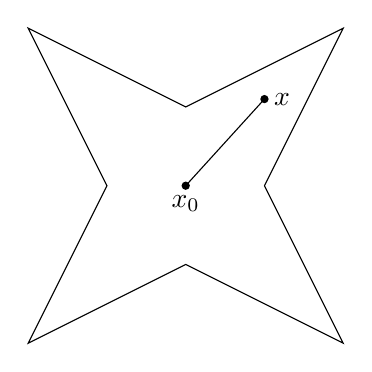
\begin{tikzpicture}
      \draw (1, 0) -- (2, 2) -- (0, 1) -- (-2, 2) -- (-1, 0) -- (-2, -2) -- (0, -1) -- (2, -2) -- (1, 0);
      \node [circ] {};
      \node [below] {$x_0$};
      \draw (0, 0) -- (1, 1.1) node [circ] {} node [right] {$x$};
    \end{tikzpicture}
  \end{center}
  We define $F_t: U \to U$ by
  \[
    F_t(x) = tx + (1 - t) x_0.
  \]
  Then $F$ is a smooth homotopy from the identity map to $F_0$, the constant map to $x_0$. We clearly have $F_1^*$ being the identity map, and $F_0^*$ is the zero map on $H^p_{\dR}(U)$ for all $p \geq 1$. So we have
  \[
    H_{\dR}^p(U) =
    \begin{cases}
      0 & p \geq 1\\
      \R & p = 0
    \end{cases}.
  \]
\end{eg}

\begin{cor}[Poincar\'e lemma]\index{Poincar\'e lemma}
  Let $U \subseteq \R^n$ be open and star-shaped. Suppose $\omega \in \Omega^p(U)$ is such that $\d \omega = 0$. Then there is some $\sigma \in \Omega^{p - 1}(M)$ such that $\omega = \d \sigma$.
\end{cor}

\begin{proof}
  $H^p_{\dR}(U) = 0$ for $p \geq 1$.
\end{proof}

More generally, we have the following notion.

\begin{defi}[Smooth homotopy equivalence]\index{smooth homotopy equivalence}
  We say two manifolds $M, N$ are \emph{smoothly homotopy equivalent} if there are smooth maps $F: M \to N$ and $G: N \to M$ such that both $F \circ G$ and $G \circ F$ are homotopic to the identity.
\end{defi}

\begin{cor}
  If $M$ and $N$ are smoothly homotopy equivalent, then $H_{\dR}^p(M) \cong H_{\dR}^p(N)$.
\end{cor}

Note that by approximation, it can be shown that if $M$ and $N$ are homotopy equivalent as topological spaces (i.e.\ the same definition where we drop the word ``smooth''), then they are in fact smoothly homotopy equivalent. So the de Rham cohomology depends only on the homotopy type of the underlying topological space.

\subsection{Homological algebra and Mayer-Vietoris theorem}
The main theorem we will have for computing de Rham cohomology will be the Mayer-Vietoris theorem. Proving this involves quite a lot of setting up and hard work. In particular, we need to define some notions from homological algebra to even \emph{state} Mayer-Vietoris theorem.

The actual proof will be divided into two parts. The first part is a purely algebraic result known as the \emph{snake lemma}, and the second part is a differential-geometric part that proves that we satisfy the hypothesis of the snake lemma.

We will not prove the snake lemma, whose proof can be found in standard algebraic topology texts (perhaps with arrows the wrong way round). % include this!

We start with some definitions.
\begin{defi}[Cochain complex and exact sequence]\index{cochain complex}\index{exact sequence}
  A sequence of vector spaces and linear maps
  \[
    \begin{tikzcd}
      \cdots \ar[r] & V^{p - 1} \ar[r, "\d_{p - 1}"] & V^p \ar[r, "\d_p"] & V^{p + 1} \ar[r] & \cdots
    \end{tikzcd}
  \]
  is a \emph{cochain complex} if $\d_p \circ \d_{p - 1} = 0$ for all $p \in \Z$. Usually we have $V^p = 0$ for $p < 0$ and we do not write them out. Keeping these negative degree $V^p$ rather than throwing them away completely helps us state our theorems more nicely, so that we don't have to view $V^0$ as a special case when we state our theorems.

  It is \emph{exact at $p$} if $\ker \d_p = \im \d_{p - 1}$, and \emph{exact} if it is exact at every $p$.
\end{defi}
There are, of course, chain complexes as well, but we will not need them for this course.

\begin{eg}
  The \term{de Rham complex}
  \[
    \begin{tikzcd}
      \Omega^0(M) \ar[r, "\d"] & \Omega^1(M) \ar[r, "\d"] & \Omega^2(M) \ar[r] & \cdots
    \end{tikzcd}
  \]
  is a cochain complex as $\d^2 = 0$. It is exact at $p$ iff $H_{\dR}^p(M) = \{0\}$.
\end{eg}

\begin{eg}
  If we have an exact sequence such that $\dim V^p < \infty$ for all $p$ and are zero for all but finitely many $p$, then
  \[
    \sum_p (-1)^p \dim V^p = 0.
  \]
\end{eg}

\begin{defi}[Cohomology]\index{cohomology}
  Let
  \[
    V^{\Cdot} =
    \begin{tikzcd}
      \cdots \ar[r] & V^{p - 1} \ar[r, "\d_{p - 1}"] & V^p \ar[r, "\d_p"] & V^{p + 1} \ar[r] & \cdots
    \end{tikzcd}
  \]
  be a cochain complex. The \emph{cohomology} of $V^{\Cdot}$ at $p$ is given by
  \[
    H^p(V^{\Cdot}) = \frac{\ker \d_p}{\im \d_{p - 1}}.
  \]
\end{defi}

\begin{eg}
  The cohomology of the de Rham complex is the de Rham cohomology.
\end{eg}

We can define maps between cochain complexes:
\begin{defi}[Cochain map]\index{cochain map}
  Let $V^{\Cdot}$ and $W^\Cdot$ be cochain complexes. A \emph{cochain map} $V^{\Cdot} \to W^{\Cdot}$ is a collection of maps $f^p: V^p \to W^p$ such that the following diagram commutes for all $p$:
   \[
     \begin{tikzcd}
       V^p \ar[r, "f^p"] \ar[d, "\d_p"] & W^p \ar[d, "\d_p"]\\
       V^{p + 1} \ar[r, "f^{p + 1}"] & W^{p + 1}
     \end{tikzcd}
   \]
\end{defi}

\begin{prop}
  A cochain map induces a well-defined homomorphism on the cohomology groups.
\end{prop}

\begin{defi}[Short exact sequence]
  A \term{short exact sequence} is an exact sequence of the form
  \[
    \begin{tikzcd}
      0 \ar[r] & V^1 \ar[r, "\alpha"] & V^2 \ar[r, "\beta"] & V^3 \ar[r] & 0
    \end{tikzcd}.
  \]
  This implies that $\alpha$ is injective, $\beta$ is surjective, and $\im (\alpha) = \ker(\beta)$. By the rank-nullity theorem, we know
  \[
    \dim V^2 = \rank(\beta) + \mathrm{null}(\beta) = \dim V^3 + \dim V^1.
  \]
\end{defi}

We can now state the main technical lemma, which we shall not prove.
\begin{thm}[Snake lemma]\index{snake lemma}
  Suppose we have a short exact sequence of complexes
  \[
    \begin{tikzcd}
      0 \ar[r] & A^{\Cdot} \ar [r, "i"] & B^{\Cdot} \ar [r, "q"] & C^{\Cdot} \ar[r] & 0
    \end{tikzcd},
  \]
  i.e.\ the $i, q$ are cochain maps and we have a short exact sequence
  \[
    \begin{tikzcd}
      0 \ar[r] & A^p \ar [r, "i^p"] & B^p \ar [r, "q^p"] & C^p \ar[r] & 0
    \end{tikzcd},
  \]
  for each $p$.

  Then there are maps
  \[
    \delta: H^p(C^{\Cdot}) \to H^{p + 1}(A^{\Cdot})
  \]
  such that there is a long exact sequence
  \[
    \begin{tikzcd}
      \cdots \ar [r] & H^p(A^{\Cdot}) \ar[r, "i^*"] & H^p(B^{\Cdot}) \ar[r, "q^*"] & H^p(C^{\Cdot}) \ar[out=0, in=180, looseness=2, overlay, dll, "\delta"']\\
      & H^{p + 1}(A^{\Cdot}) \ar[r, "i^*"] & H^{p + 1}(B^{\Cdot}) \ar[r, "q^*"] & H^{p + 1}(C^{\Cdot}) \ar [r] & \cdots
    \end{tikzcd}.
  \]
\end{thm}

Using this, we can prove the Mayer-Vietoris theorem.
\begin{thm}[Mayer-Vietoris theorem]\index{Mayer-Vietoris sequence}
  Let $M$ be a manifold, and $M = U \cup V$, where $U, V$ are open. We denote the inclusion maps as follows:
  \[
    \begin{tikzcd}
      U \cap V \ar[r, "i_1", hook] \ar[d, "i_2", hook] & U \ar[d, hook, "j_1"]\\
      V \ar[r, hook, "j_2"] & M
    \end{tikzcd}
  \]
  Then there exists a natural linear map
  \[
    \delta: H^p_\dR (U \cap V) \to H_{\dR}^{p + 1}(M)
  \]
  such that the following sequence is exact:
  \[
    \begin{tikzcd}
      H^p_{\dR}(M) \ar[r, "j_1^* \oplus j_2^*"] & H^p_{\dR}(U) \oplus H^p_{\dR}(V) \ar[r, "i_1^* - i_2^*"] & H_\dR^p(U \cap V)\ar[out=0, in=180, looseness=2, overlay, lld, "\delta"]\\
      H_\dR^{p+1}(M) \ar[r, "j_1^* \oplus j_2^*"] & H_\dR^{p+1}(U) \oplus H_\dR^{p+1}(V) \ar[r, "i_1^* - i_2^*"] & \cdots
    \end{tikzcd}
  \]
\end{thm}

Before we prove the theorem, we do a simple example.
\begin{eg}
  Consider $M = S^1$. We can cut the circle up:
  \begin{center}
    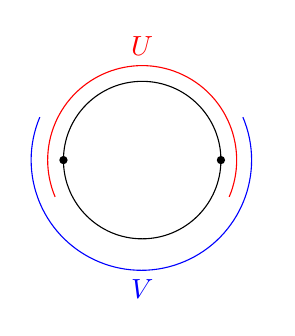
\begin{tikzpicture}
      \draw circle [radius=1];
      \draw [red] (1.105, -0.4673) arc(-22.9:202.9:1.2);
      \node [red, above] at (0, 1.2) {$U$};

      \draw [blue] (1.279, 0.545) arc(22.9:-202.9:1.4);
      \node [blue, below] at (0, -1.4) {$V$};

      \node [circ] at (1, 0) {};
      \node [circ] at (-1, 0) {};
    \end{tikzpicture}
  \end{center}
  Here we have
  \begin{align*}
    S^1 &= \{(x, y): x^2 + y^2 = 1\}\\
    U &= S^1 \cap \{y > -\varepsilon\}\\
    V &= S^1 \cap \{y < \varepsilon\}.
  \end{align*}
  As $U, V$ are diffeomorphic to intervals, hence contractible, and $U \cap V$ is diffeomorphic to the disjoint union of two intervals, we know their de Rham cohomology.
  \[
    \begin{tikzcd}
      0 \ar[r] & H^0_{\dR}(S^1) \ar[r] & H^0_{\dR}(U) \oplus H^0_{\dR}(V) \ar[r] & H_\dR^0(U \cap V)\ar[out=0, in=180, looseness=2, overlay, lld]\\
      & H_\dR^1(S^1) \ar[r] & H_\dR^1(U) \oplus H_\dR^1(V) \ar[r] & \cdots
    \end{tikzcd}
  \]
  We can fill in the things we already know to get
  \[
    \begin{tikzcd}
      0 \ar[r] & \R \ar[r] & \R \oplus \R \ar[r] & \R \oplus \R\ar[out=0, in=180, looseness=2, overlay, lld]\\
      & H_\dR^1(S^1) \ar[r] & 0 \ar[r] & \cdots
    \end{tikzcd}
  \]
  By adding the degrees alternatingly, we know that
  \[
    \dim H^1_{\dR}(S^1) = 1.
  \]
  So
  \[
    H^1_{\dR}(S^1) \cong \R.
  \]
\end{eg}

Now we prove Mayer-Vietoris.

\begin{proof}[Proof of Mayer-Vietoris]
  By the snake lemma, it suffices to prove that the following sequence is exact for all $p$:
  \[
    \begin{tikzcd}
      0 \ar[r] & \Omega^p(U \cup V) \ar[r, "j_1^* \oplus j_2^*"] & \Omega^p(U) \oplus \Omega^p(V) \ar[r, "i_1^* - i_2^*"] & \Omega^p(U \cap V) \ar[r] & 0
    \end{tikzcd}
  \]
  It is clear that the two maps compose to $0$, and the first map is injective. By counting dimensions, it suffices to show that $i_1^* - i_2^*$ is surjective.

  Indeed, let $\{\varphi_U, \varphi_V\}$ be partitions of unity subordinate to $\{U, V\}$. Let $\omega \in \Omega^p(U \cap V)$. We set $\sigma_U \in \Omega^p(U)$ to be
  \[
    \sigma_U =
    \begin{cases}
      \varphi_V \omega & \text{on }U \cap V\\
      0 & \text{on }U \setminus \supp \varphi_V
    \end{cases}.
  \]
  Similarly, we define $\sigma_V \in \Omega^p(V)$ by
  \[
    \sigma_V =
    \begin{cases}
      -\varphi_U \omega & \text{on }U \cap V\\
      0 & \text{on }V \setminus \supp \varphi_U
    \end{cases}.
  \]
  Then we have
  \[
    i_1^* \sigma_U - i_2^* \sigma_V = (\varphi_V \omega + \varphi_U \omega)|_{U \cap V} = \omega.
  \]
  So $i_1^* - i_2^*$ is surjective.
\end{proof}

\section{Integration}
As promised, we will be able to integrate differential forms on manifolds. However, there is a slight catch. We said that differential forms give us the signed volume of an infinitesimal parallelepiped, and we can integrate these infinitesimal volumes up to get the whole volume of the manifold. However, there is no canonical choice of the sign of the volume, so we do not, in general, get a well-defined volume.

In order to fix this issue, our manifold needs to have an \emph{orientation}.

\subsection{Orientation}
We start with the notion of an orientation of a vector space. After we have one, we can define an orientation of a manifold to be a smooth choice of orientation for each tangent space.

Informally, an orientation on a vector space $V$ is a choice of a collection of ordered bases that we declare to be ``oriented''. If $(e_1, \cdots, e_n)$ is an oriented basis, then changing the sign of one of the $e_i$ changes orientation, while scaling by a positive multiple does not. Similarly, swapping two elements in the basis will induce a change in orientation.

To encode this information, we come up with some alternating form $\omega \in \Lambda^n(V^*)$. We can then say a basis $e_1, \cdots, e_n$ is oriented if $\omega(e_1, \cdots, e_n)$ is positive.

\begin{defi}[Orientation of vector space]\index{orientation!vector space}
  Let $V$ be a vector space with $\dim V = n$. An \emph{orientation} is an equivalence class of elements $\omega \in\Lambda^n (V^*)$, where we say $\omega \sim \omega'$ iff $\omega = \lambda \omega'$ for some $\lambda > 0$. A basis $(e_1, \cdots, e_n)$ is \emph{oriented} if
  \[
    \omega(e_1, \cdots, e_n) > 0.
  \]
  By convention, if $V = \{0\}$, an orientation is just a choice of number in $\{\pm 1\}$.
\end{defi}

Suppose we have picked an oriented basis $e_1, \cdots, e_n$. If we have any other basis $\tilde{e}_1, \cdots, \tilde{e}_n$, we write
\[
  e_i = \sum_j B_{ij} \tilde{e}_j.
\]
Then we have
\[
  \omega (\tilde{e}_1, \cdots, \tilde{e}_n) = \det B\; \omega(e_1, \cdots, e_n).
\]
So $\tilde{e}_1, \cdots, \tilde{e}_n$ is oriented iff $\det B > 0$.

We now generalize this to manifolds, where we try to orient the tangent bundle smoothly.

\begin{defi}[Orientation of a manifold]\index{orientation!manifold}\index{manifold!orientation}
  An \emph{orientation} of a manifold $M$ is defined to be an equivalence class of elements $\omega \in \Omega^n(M)$ that are nowhere vanishing, under the equivalence relation $ \omega \sim \omega'$ if there is some smooth $f: M \to \R_{> 0}$ such that $\omega = f \omega'$.
\end{defi}

\begin{defi}[Orientable manifold]\index{orientable manifold}\index{manifold!orientable}
  A manifold is \emph{orientable} if it has some orientation.
\end{defi}

If $M$ is a connected, orientable manifold, then it has precisely two possible orientations.

\begin{defi}[Oriented manifold]\index{oriented manifold}
  An \emph{oriented manifold} is a manifold with a choice of orientation.
\end{defi}

\begin{defi}[Oriented coordinates]\index{oriented coordinates}
  Let $M$ be an oriented manifold. We say coordinates $x_1, \cdots, x_n$ on a chart $U$ are \emph{oriented coordinates} if
  \[
    \left.\frac{\partial}{\partial x_1}\right|_p, \cdots, \left.\frac{\partial}{\partial x_n}\right|_p
  \]
  is an oriented basis for $T_p M$ for all $p \in U$.
\end{defi}
Note that we can always find enough oriented coordinates. Given any connected chart, either the chart is oriented, or $-x_1, \cdots, x_n$ is oriented. So any oriented $M$ is covered by oriented charts.

Now by the previous discussion, we know that if $x_1, \cdots, x_n$ and $y_1, \cdots, y_n$ are oriented charts, then the transition maps for the tangent space all have positive determinant.

\begin{eg}
  $\R^n$ is always assumed to have the standard orientation given by $\d x_1 \wedge \cdots \wedge \d x_n$.
\end{eg}

\begin{defi}[Orientation-preserving diffeomorphism]\index{orientation!-preserving diffeomorphism}\index{diffeomorphism!orientation preserving}
  Let $M, N$ be oriented manifolds, and $F \in C^\infty(M, N)$ be a diffeomorphism. We say $F$ \emph{preserves orientation} if $\D F|_p: T_p M \to T_{F(p)}N$ takes an oriented basis to an oriented basis.

  Alternatively, this says the pullback of the orientation on $N$ is the orientation on $M$ (up to equivalence).
\end{defi}

\subsection{Integration}
The idea is that to define integration, we fist understand how we can integrate on $\R^n$, and then patch them up using partitions of unity.

We are going to allow ourselves to integrate on rather general domains.
\begin{defi}[Domain of integration]\index{domain of integration}
  Let $D \subseteq \R^n$. We say $D$ is a \emph{domain of integration} if $D$ is bounded and $\partial D$ has measure zero.
\end{defi}

Since $D$ can be an arbitrary subset, we define an $n$-form on $D$ to be some $\omega \in \Omega^n(U)$ for some open $U$ containing $D$.

\begin{defi}[Integration on $\R^n$]\index{integration!on $\R^n$}
  Let $D$ be a compact domain of integration, and
  \[
    \omega = f\; \d x_1 \wedge \cdots \wedge \d x_n
  \]
  be an $n$-form on $D$. Then we define
  \[
    \int_D \omega = \int_D f(x_1, \cdots, x_n) \;\d x_1 \cdots \d x_n.
  \]
  In general, let $U \subseteq \R^n$ and let $\omega \in \Omega^n(\R^n)$ have compact support. We define
  \[
    \int_U \omega = \int_D \omega
  \]
  for some $D\subseteq U$ containing $\supp \omega$.
\end{defi}
Note that we do not directly say we integrate it on $\supp \omega$, since $\supp \omega$ need not have a nice boundary.

Now if we want to integrate on a manifold, we need to patch things up, and to do so, we need to know how these things behave when we change coordinates.

\begin{defi}[Smooth function]\index{smooth function}
  Let $D \subseteq \R^n$ and $f: D \to \R^m$. We say $f$ is \emph{smooth} if it is a restriction of some smooth function $\tilde{f}: U \to \R^m$ where $U \supseteq D$.
\end{defi}

\begin{lemma}
  Let $F: D \to E$ be a smooth map between domains of integration in $\R^n$, and assume that $F|_{\mathring{D}}: \mathring{D} \to \mathring{E}$ is an orientation-preserving diffeomorphism. Then
  \[
    \int_E \omega = \int_D F^* \omega.
  \]
\end{lemma}
This is exactly what we want.

\begin{proof}
  Suppose we have coordinates $x_1, \cdots, x_n$ on $D$ and $y_1, \cdots, y_n$ on $E$. Write
  \[
    \omega = f\;\d y_1 \wedge \cdots \wedge \d y_n.
  \]
  Then we have
  \begin{align*}
    \int_E \omega &= \int_E f\;\d y_1 \cdots \d y_n\\
    &= \int_D (f \circ F)\, |\det \D F|\;\d x_1 \cdots \d x_n\\
    &= \int_D (f \circ F) \det \D F \; \d x_1 \cdots \d x_n\\
    &= \int_D F^* \omega.
  \end{align*}
  Here we used the fact that $|\det \D F| = \det \D F$ because $F$ is orientation-preserving.
\end{proof}

We can now define integration over manifolds.

\begin{defi}[Integration on manifolds]\index{integration!manifolds}
  Let $M$ be an oriented manifold. Let $\omega \in \Omega^n(M)$. Suppose that $\supp(\omega)$ is a compact subset of some oriented chart $(U, \varphi)$. We set
  \[
    \int_M \omega = \int_{\varphi(U)} (\varphi^{-1})^* \omega.
  \]
  By the previous lemma, this does not depend on the oriented chart $(U, \varphi)$.

  If $\omega \in \Omega^n(M)$ is a general form with compact support, we do the following: cover the support by finitely many oriented charts $\{U_\alpha\}_{\alpha = 1, \ldots, m}$. Let $\{\chi_\alpha\}$ be a partition of unity subordinate to $\{U_\alpha\}$. We then set
  \[
    \int_M \omega = \sum_\alpha \int_{U_\alpha} \chi_\alpha \omega.
  \]
\end{defi}

It is clear that we have
\begin{lemma}
  This is well-defined, i.e.\ it is independent of cover and partition of unity.
\end{lemma}
We will not bother to go through the technicalities of proving this properly.

Note that it is possible to define this for non-smooth forms, or not-everywhere-defined form, or with non-compact support etc, but we will not do it here.

Theoretically, our definition is perfectly fine and easy to work with. However, it is absolutely useless for computations, and there is no hope you can evaluate that directly.

Now how would we \emph{normally} integrate things? In IA Vector Calculus, we probably did something like this --- if we want to integrate something over a sphere, we cut the sphere up into the Northern and Southern hemisphere. We have coordinates for each of the hemispheres, so we integrate each hemisphere separately, and then add the result up.

This is all well, except we have actually missed out the equator in this process. But that doesn't really matter, because the equator has measure zero, and doesn't contribute to the integral.

We now try to formalize our above approach. The below definition is not standard:
\begin{defi}[Parametrization]\index{parametrization}
  Let $M$ be either an oriented manifold of dimension $n$, or a domain of integration in $\R^n$. By a \emph{parametrization} of $M$ we mean a decomposition
  \[
    M = S_1 \cup \cdots \cup S_n,
  \]
  with smooth maps $F_i: D_i \to S_i$, where $D_i$ is a compact domain of integration, such that
  \begin{enumerate}
    \item $F_i|_{\mathring{D}_i}: \mathring{D}_i \to \mathring{S}_i$ is an orientation-preserving diffeomorphism
    \item $\partial S_i$ has measure zero (if $M$ is a manifold, this means $\varphi(\partial S_i \cap U)$ for all charts $(U, \varphi)$).
    \item For $i \not= j$, $S_i$ intersects $S_j$ only in their common boundary.
  \end{enumerate}
\end{defi}

\begin{thm}
  Given a parametrization $\{S_i\}$ of $M$ and an $\omega \in \Omega^n(M)$ with compact support, we have
  \[
    \int_M \omega = \sum_i \int_{D_i} F_i^* \omega.
  \]
\end{thm}

\begin{proof}
% We know $M$ is covered by oriented charts $(U_\alpha, \varphi_\alpha)$ such that $\varphi$ gives a smooth map $\varphi: \bar{U}_\alpha \to \overline{B_1(0)}$. We can then pick this cover and a partition of unity subordinate to this cover. Then if we define $\int_M \omega$ this way, it suffices to deal with the case where $\supp(\omega)$ lies in a single chart $(U, \varphi)$. Then identifying $\bar{U}$ with $\overline{B_1(0)}$, it suffices to consider the case where $M = \overline{B_1(0)}$. Then the result is obvious.

  By using partitions of unity, we may consider the case where $\omega$ has support in a single chart, and thus we may wlog assume we are working on $\R^n$, and then the result is obvious.
\end{proof}

There is a problem --- in all our lives, we've been integrating functions, not forms. If we have a function $f: \R \to \R$, then we can take the integral
\[
  \int f\;\d x.
\]
Now of course, we are not actually integrating $f$. We are integrating the differential form $f\;\d x$. Why we seem like we are integrating functions is because we have a background form $\d x$. So if we have a manifold $M$ with a ``background'' $n$-form $\omega \in \Omega^n (M)$, then we can integrate $f \in C^\infty(M, \R)$ by
\[
  \int_M f \omega.
\]
In general, a manifold does not come with such a canonical background form. However, in some cases, it does.
\begin{lemma}
  Let $M$ be an oriented manifold, and $g$ a Riemannian metric on $M$. Then there is a unique $\omega \in \Omega^n(M)$ such that for all $p$, if $e_1, \cdots, e_n$ is an oriented orthonormal basis of $T_pM$, then
  \[
    \omega(e_1, \cdots, e_n) = 1.
  \]
  We call this the \term{Riemannian volume form}, written \term{$\d V_g$}.
\end{lemma}
Note that $\d V_g$ is a notation. It is not the exterior derivative of some mysterious object $V_g$.

\begin{proof}
  Uniqueness is clear, since if $\omega'$ is another, then $\omega_p = \lambda \omega'_p$ for some $\lambda$, and evaluating on an orthonormal basis shows that $\lambda = 1$.

  To see existence, let $\sigma$ be any nowhere vanishing $n$-form giving the orientation of $M$. On a small set $U$, pick a frame $s_1, \cdots, s_n$ for $TM|_U$ and apply the Gram-Schmidt process to obtain an orthonormal frame $e_1, \cdots, e_n$, which we may wlog assume is oriented. Then we set
  \[
    f = \sigma(e_1, \cdots, e_n),
  \]
  which is non-vanishing because $\sigma$ is nowhere vanishing. Then set
  \[
    \omega = \frac{\sigma}{f}.
  \]
  This proves existence locally, and can be patched together globally by uniqueness.
\end{proof}
\subsection{Stokes Theorem}
Recall from, say, IA Vector Calculus that Stokes' theorem relates an integral on a manifold to a integral on its boundary. However, our manifolds do not have boundaries! So we can't talk about Stokes' theorem! So we now want to define what it means to be a manifold with boundary.

\begin{defi}[Manifold with boundary]\index{manifold!with boundary}\index{chart!with boundary}\index{atlas!with boundary}
  Let
  \[
    \H^n = \{(x_1, \cdots, x_n)\in \R^n: x_n \geq 0\}.
  \]
  A \emph{chart-with-boundary} on a set $M$ is a bijection $\varphi: U \to \varphi(U)$ for some $U \subseteq M$ such that $\varphi(U) \subseteq \H^n$ is open. Note that this image may or may not hit the boundary of $\H^n$. So a ``normal'' chart is also a chart with boundary.

  An \emph{atlas-with-boundary} on $M$ is a cover by charts-with-boundary $(U_\alpha, \varphi_\alpha)$ such that the transition maps
  \[
    \varphi_\beta \circ \varphi_\alpha^{-1}: \varphi_\alpha(U_\alpha \cap U_\beta) \to \varphi_\beta(U_\alpha \cap U_\beta)
  \]
  are smooth (in the usual sense) for all $\alpha, \beta$.

  A \emph{manifold-with-boundary} is a set $M$ with an (equivalence class of) atlas with boundary whose induced topology is Hausdorff and second-countable.
\end{defi}

Note that a manifold with boundary is not a manifold, but a manifold is a manifold with boundary. We will often be lazy and drop the ``with boundary'' descriptions.

\begin{defi}[Boundary point]\index{boundary point}\index{$\partial M$}
  If $M$ is a manifold with boundary and $p \in M$, then we say $p$ is a \emph{boundary point} if $\varphi(p) \in \partial \H^n$ for some (hence any) chart-with-boundary $(U, \varphi)$ containing $p$. We let $\partial M$ be the set of boundary points and $\Int(M) = M \setminus \partial M$.
\end{defi}

Note that these are not the topological notions of boundary and interior.

\begin{prop}
  Let $M$ be a manifold with boundary. Then $\Int(M)$ and $\partial M$ are naturally manifolds, with
  \[
    \dim \partial M = \dim \Int M - 1.
  \]
\end{prop}

\begin{eg}
  The solid ball $\overline{B_1(0)}$ is a manifold with boundary, whose interior is $B_1(0)$ and boundary is $S^{n - 1}$.
\end{eg}

Note that the product of manifolds with boundary is not a manifold with boundary. For example, the interval $[0, 1]$ is a manifold with boundary, but $[0, 1]^2$ has \emph{corners}. This is bad. We can develop the theory of manifolds with corners, but that is more subtle. We will not talk about them.

Everything we did for manifolds can be done for manifolds with boundary, e.g.\ smooth functions, tangent spaces, tangent bundles etc. Note in particular the definition of the tangent space as derivations still works word-for-word.

\begin{lemma}
  Let $p \in \partial M$, say $p \in U \subseteq M$ where $(U, \varphi)$ is a chart (with boundary). Then
  \[
    \left.\frac{\partial }{\partial x_1}\right|_p, \cdots, \left.\frac{\partial}{\partial x_n}\right|_p
  \]
  is a basis for $T_p M$. In particular, $\dim T_p M = n$.
\end{lemma}

\begin{proof}
  Since this is a local thing, it suffices to prove it for $M = \H^n$. We write $C^\infty(\H, \R)$ for the functions $f: \H^n \to \R^n$ that extend smoothly to an open neighbourhood of $\H^n$. We fix $a \in \partial \H^n$. Then by definition, we have
  \[
    T_a\H^n = \Der_a(C^\infty(\H^n, \R)).
  \]
  We let $i_*: T_a\H^n \to T_a \R^n$ be given by
  \[
    i_*(X) (g) = X(g|_{\H^n})
  \]
  We claim that $i_*$ is an isomorphism. For injectivity, suppose $i_*(X) = 0$. If $f \in C^\infty(\H^n)$, then $f$ extends to a smooth $g$ on some neighbourhood $U$ of $\H^n$. Then
  \[
    X(f) = X(g|_{\H^n}) = i_*(X)(g) = 0.
  \]
  So $X(f) = 0$ for all $f$. Then $X = 0$. So $i_*$ is injective.

  To see surjectivity, let $Y \in T_a \R^n$, and let $X \in T_a\H^n$ be defined by
  \[
    X(f) = Y(g),
  \]
  where $g \in C^\infty(\H^n, \R)$ is any extension of $f$ to $U$. To see this is well-defined, we let
  \[
    Y = \sum_{i=1}^n \alpha_i \left.\frac{\partial}{\partial x_i}\right|_a.
  \]
  Then
  \[
    Y(g) = \sum_{i=1}^n \alpha_i \frac{\partial g}{\partial x_i}(a),
  \]
  which only depends on $g|_{\H^n}$, i.e.\ $f$. So $X$ is a well-defined element of $T_a\H^n$, and $i_*(X) = Y$ by construction. So done.
\end{proof}

Now we want to see how orientations behave. We can define them in exactly the same way as manifolds, and everything works. However, something interesting happens. If a manifold with boundary has an orientation, this naturally induces an orientation of the boundary.
\begin{defi}[Outward/Inward pointing]\index{outward pointing}\index{inward pointing}
  Let $p \in \partial M$. We then have an inclusion $T_p \partial M \subseteq T_p M$. If $X_p \in T_p M$, then in a chart, we can write
  \[
    X_p = \sum_{i = 1}^n a_i \frac{\partial}{\partial x_i},
  \]
  where $a_i \in \R$ and $\frac{\partial}{\partial x_1}, \cdots, \frac{\partial}{\partial x_{n - 1}}$ are a basis for $T_p \partial M$. We say $X_p$ is \emph{outward pointing} if $a_n < 0$, and \emph{inward pointing} if $a_n > 0$.
\end{defi}

\begin{defi}[Induced orientation]\index{induced orientation}
  Let $M$ be an oriented manifold with boundary. We say a basis $e_1,\cdots, e_{n - 1}$ is an oriented basis for $T_p \partial M$ if $(X_p, e_1, \cdots, e_{n - 1})$ is an oriented basis for $T_p M$, where $X_p$ is any outward pointing element in $T_p M$. This orientation is known as the \emph{induced orientation}.
\end{defi}

It is an exercise to see that these notions are all well-defined and do not depend on the basis.
\begin{eg}
  We have an isomorphism
  \begin{align*}
    \partial\H^n &\cong \R^{n - 1}\\
    (x_1, \cdots, x_{n - 1}, 0) &\mapsto (x_1, \cdots, x_{n - 1}).
  \end{align*}
  So
  \[
    \left.-\frac{\partial}{\partial x_n}\right|_{\partial \H^n}
  \]
  is an outward pointing vector. So we know $x_1, \cdots, x_{n - 1}$ is an oriented chart for $\partial \H^n$ iff
  \[
    -\frac{\partial}{\partial x_n}, \frac{\partial}{\partial x_1}, \cdots, \frac{\partial}{\partial x_{n-1}}
  \]
  is oriented, which is true iff $n$ is even.
\end{eg}

\begin{eg}
  If $n = 1$, say $M = [a, b] \subseteq \R$ with $a < b$, then $\{a, b\}$, then $T_p \partial M = \{0\}$. So an orientation of $\partial M$ is a choice of numbers $\pm 1$ attached to each point. The convention is that if $M$ is in the standard orientation induced by $M \subseteq \R$, then the orientation is obtained by giving $+1$ to $b$ and $-1$ to $a$.
\end{eg}

Finally, we get to Stokes' theorem.
\begin{thm}[Stokes' theorem]\index{Stokes' theorem}
  Let $M$ be an oriented manifold with boundary of dimension $n$. Then if $\omega \in \Omega^{n - 1}(M)$ has compact support, then
  \[
    \int_M \d \omega = \int_{\partial M}\omega.
  \]
  In particular, if $M$ has no boundary, then
  \[
    \int_M \d \omega = 0
  \]
\end{thm}
Note that this makes sense. $\d \omega$ is an $n$-form on $M$, so we can integrate it. On the right hand side, what we really doing is integrating the restriction of $\omega$ to $\partial M$, i.e.\ the $(n - 1)$-form $i^* \omega$, where $i: \partial M \to M$ is the inclusion, so that $i^* \omega \in \Omega^{n - 1}(\partial M)$.

Note that if $M = [a, b]$, then this is just the usual fundamental theorem of calculus.

The hard part of the proof is keeping track of the signs.
\begin{proof}
  We first do the case where $M = \H^n$. Then we have
  \[
    \omega = \sum_{i = 1}^n \omega_i\;\d x_1 \wedge \cdots \wedge \widehat{\d x_i} \wedge \cdots \wedge \d x_n,
  \]
  where $\omega_i$ is compactly supported, and the hat denotes omission. So we have
  \begin{align*}
    \d \omega &= \sum_i \d \omega_i \wedge \d x_1 \wedge \cdots \wedge \widehat{\d x_i} \wedge \cdots \wedge \d x_n\\
    &= \sum_i \frac{\partial \omega_i}{\partial x_i} \d x_i \wedge \d x_1 \wedge \cdots \wedge \widehat{\d x_i} \wedge \cdots \wedge \d x_n\\
    &= \sum_i (-1)^{i - 1} \frac{\partial \omega_i}{\partial x_i} \d x_1 \wedge \cdots \wedge \d x_i \wedge \cdots \wedge \d x_n
  \end{align*}
  Let's say
  \[
    \supp(\omega) = \{x_j \in [-R, R]: j = 1, \cdots, n - 1; x_n \in [0, R]\} = A.
  \]
  Then suppose $i \not= n$. Then we have
  \begin{align*}
    &\hphantom{=}\int_{\H^n} \frac{\partial \omega_i}{\partial x_i} \d x_1 \wedge \cdots \wedge \d x_i \wedge \cdots \wedge \d x_n\\
    &= \int_A \frac{\partial \omega_i}{\partial x_i} \d x_1 \cdots \d x_n\\
    &= \int_{-R}^R \int_{-R}^R \cdots \int_{-R}^R \int_0^R \frac{\partial\omega_i}{\partial x_i}\;\d x_1 \cdots \d x_n\\
    \intertext{By Fubini's theorem, we can integrate this in any order. We integrate with respect to $\d x_i$ first. So this is}
    &= \pm \int_{-R}^R \cdots \int_{-R}^R \int_0^R \left(\int_{-R}^R \frac{\partial \omega_i}{\partial x_i}\;\d x_i\right)\d x_1 \cdots \widehat{\d x_i} \cdots \d x_n
  \end{align*}
  By the fundamental theorem of calculus, the inner integral is
  \[
    \omega(x_1, \cdots, x_{i - 1}, R, x_{i + 1}, \cdots, x_n) - \omega(x_1, \cdots, x_{i - 1}, -R, x_{i + 1}, \cdots, x_n) = 0 - 0 = 0.
  \]
  So the integral vanishes. So we are only left with the $i = n$ term. So we have
  \begin{align*}
    \int_{\H^n} \d \omega &= (-1)^{n - 1} \int_A \frac{\partial \omega_n}{\partial x_n} \;\d x_1 \cdots \d x_n\\
    &= (-1)^{n - 1} \int_{-R}^R \cdots \int_{-R}^R \left(\int_0^R \frac{\partial \omega_n}{\partial x_n}\;\d x_n\right) \d x_1 \cdots \d x_{n - 1}
  \end{align*}
  Now that integral is just
  \[
    \omega_n(x_1, \cdots, x_{n - 1}, R) - \omega_n(x_1, \cdots, x_{n - 1}, 0) = -\omega_n(x_1, \cdots, x_{n - 1}, 0).
  \]
  So this becomes
  \[
    =(-1)^n \int_{-R}^R \cdots \int_{-R}^R \omega_n(x_1, \cdots, x_{n - 1}, 0)\;\d x_1 \cdots \d x_{n - 1}.
  \]
  Next we see that
  \[
    i^* \omega = \omega_n \d x_1 \wedge \cdots \wedge \d x_{n - 1},
  \]
  as $i^*(\d x_n) = 0$. So we have
  \[
    \int_{\partial \H^n} i^* \omega = \pm \int_{A \cap \partial \H^n} \omega(x_1, \cdots, x_{n - 1}, 0) \, \d x_1 \cdots \d x_n.
  \]
  Here the sign is a plus iff $x_1, \cdots, x_{n - 1}$ are an oriented coordinate for $\partial \H^n$, i.e.\ $n$ is even. So this is
  \[
    \int_{\partial \H^n} \omega = (-1)^n \int_{-R}^R \cdots \int_{-R}^R \omega_n(x_1, \cdots, x_{n - 1}, 0)\;\d x_1 \cdots \d x_{n - 1} = \int_{\H^n} \d \omega.
  \]
  Now for a general manifold $M$, suppose first that $\omega \in \Omega^{n - 1}(M)$ is compactly supported in a single oriented chart $(U, \varphi)$. Then the result is true by working in local coordinates. More explicitly, we have
  \[
    \int_M \d \omega = \int_{\H^n}(\varphi^{-1})^* \d \omega = \int_{\H^n} \d((\varphi^{-1})^* \omega) = \int_{\partial \H^n} (\varphi^{-1})^* \omega = \int_{\partial M} \omega.
  \]
  Finally, for a general $\omega$, we just cover $M$ by oriented charts $(U, \varphi_\alpha)$, and use a partition of unity $\chi_\alpha$ subordinate to $\{U_\alpha\}$. So we have
  \[
    \omega = \sum \chi_\alpha \omega.
  \]
  Then
  \[
    \d \omega = \sum (\d \chi_\alpha) \omega + \sum \chi_\alpha \d \omega = \d\left(\sum \chi_\alpha\right) \omega + \sum \chi_\alpha \d \omega = \sum \chi_\alpha \d \omega,
  \]
  using the fact that $\sum \chi_\alpha$ is constant, hence its derivative vanishes. So we have
  \[
    \int_M \d \omega = \sum_\alpha \int_M \chi_\alpha \d \omega = \sum_\alpha \int_{\partial M} \chi_\alpha \omega = \int_{\partial M}\omega. \qedhere
  \]
\end{proof}
Then all the things likes Green's theorem and divergence theorem follow from this.

\begin{eg}
  Let $M$ be a manifold without boundary with a symplectic form $\omega \in \Omega^2(M)$ that is closed and positive definite. Then by basic Linear algebra we know
  \[
    \int_M \omega^n \not= 0.
  \]
  Since $\omega$ is closed, it is an element $[\omega] \in H_{\dR}^2 (M)$. Does this vanish? If $\omega = \d \tau$, then we have
  \[
    \d (\tau \wedge \omega \wedge \cdots \wedge \omega) = \omega^n.
  \]
  So we have
  \[
    \int_M \omega^n = \int_M \d (\tau \wedge \omega \wedge \cdots \wedge \omega) = 0
  \]
  by Stokes' theorem. This is a contradiction. So $[\omega]$ is non-zero in $H^2_{\dR}(M)$.
\end{eg}

% \subsection{Densities*}

\section{De Rham's theorem*}
In the whole section, $M$ will be a compact manifold.

\begin{thm}[de Rham's theorem]\index{de Rham's theorem}
  There exists a natural isomorphism
  \[
    H^p_{\dR}(M) \cong H^p(M, \R),
  \]
  where $H^p(M, \R)$ is the singular cohomology of $M$, and this is in fact an isomorphism of rings, where $H^p_{\dR}(M)$ has the product given by the wedge, and $H^p(M, \R)$ has the cup product.
\end{thm}

Recall that singular cohomology is defined as follow:
\begin{defi}[Singular $p$-complex]
  Let $M$ be a manifold. Then a \term{singular $p$-simplex} is a continuous map
  \[
    \sigma: \Delta_p \to M,
  \]
  where
  \[
    \Delta_p = \left\{\sum_{i = 0}^p t_i e_i: \sum t_I = 1\right\} \subseteq \R^{n + 1}.
  \]
  We define
  \[
    C_p(M) = \{\text{formal sums }\sum a_i \sigma_i: a_i \in \R, \sigma_i\text{ a singular $p$ simplex}\}.
  \]
  We define
  \[
    C_p^\infty(m) = \{\text{formal sums }\sum a_i \sigma_i: a_i \in \R, \sigma_i\text{ a smooth singular $p$ simplex}\}.
  \]
\end{defi}

\begin{defi}[Boundary map]
  The \emph{boundary map}
  \[
    \partial: C_p(M) \to C_{p - 1}(M)
  \]
  is the linear map such that if $\sigma: \Delta_p \to M$ is a $p$ simplex, then
  \[
    \partial \sigma = \sum (-1)^i \sigma \circ F_{i, p},
  \]
  where $F_{i, p}$ maps $\Delta_{p - 1}$ affine linearly to the face of $\Delta_p$ opposite the $i$th vertex. We similarly have
  \[
    \partial: C_p^\infty(M) \to C_{p - 1}^\infty(M).
  \]
\end{defi}

We can then define singular homology
\begin{defi}[Singular homology]\index{singular homology}
  The \emph{singular homology} of $M$ is
  \[
    H_p(M, \R) = \frac{\ker \partial: C_p(M) \to C_{p - 1}(M)}{\im \partial: C_{p + 1}(M) \to C_p(M)}.
  \]
  The \term{smooth singular homology}\index{singular homology!smooth} is the same thing with $C_p(M)$ replaced with $C_p^\infty(M)$.
\end{defi}

$H_p^\infty$ has the same properties as $H_p$, e.g.\ functoriality, (smooth) homotopy invariance, Mayer-Vietoris etc with no change in proof.

Any smooth $p$-simplex $\sigma$ is also continuous, giving a natural inclusion
\[
  i: C_p^\infty(M) \to C_p(M),
\]
which obviously commutes with $\partial$, giving
\[
  i_*: H_p^\infty(M) \to H_p(M).
\]
\begin{thm}
  The map $i_*: H_p^\infty(M) \to H_p(M)$ is an isomorphism.
\end{thm}

There are three ways we can prove this. We will give the ideas for these proofs:
\begin{enumerate}
  \item We can show that any continuous map $F: M \to N$ between manifolds is homotopic to a smooth one. But this is painful to prove.
  \item What we really care about is maps $\sigma: \Delta_p \to M$, and we can barycentrically subdivide the simplex so that it only lies in a single chart, and then it is easy to do smooth approximation.
  \item As $H_p$ and $H_p^\infty$ have enough properties in common, in particular they both have Mayer-Vietoris and agree on convex sets, this implies they are the same. We will not spell out this proof, because we are going to do this to prove that de Rham cohomology is the same as singular cohomology
\end{enumerate}

Since we are working with $\R$, we can cheat and define singular cohomology in a simple way:
\begin{defi}[Singular cohomology]\index{singular cohomology}
  The \emph{singular cohomology} of $M$ is defined as
  \[
    H^p(M, \R) = \Hom(H_p(M, \R), \R).
  \]
  Similarly, the smooth singular cohomology is
  \[
    H^p_\infty(M, \R) = \Hom(H_p^\infty(M, \R), \R).
  \]
\end{defi}
This is a bad definition in general! It just happens to work for singular cohomology with coefficients in $\R$, and we are not too bothered to write dowm the proper definition.

Our goal is now to describe an isomorphism
\[
  H^p_{\dR}(M) \cong H^p_\infty(M, \R).
\]
The map itself is given as follows:

Suppose $[w] \in H^p_{\dR}(M)$, so $\omega \in \Omega^p(M)$ with $\d \omega = 0$. Suppose that $\sigma: \Delta p \to M$ is smooth with $\partial \sigma = 0$. We can then define
\[
  I([\omega]) = \int_{\Delta^p} \sigma^* \omega \in \R.
\]
Note that we have not defined what $\int_{\Delta^p}$ means, because $\Delta^p$ is not even a manifold with boundary --- it has corners. We can develop an analogous theory of integration on manifolds with corners, but we can also be lazy, and just integrate over
\[
  \Delta_p^\times = \Delta_p \setminus \{\text{codimension 2 faces}\}.
\]
Now $\omega|_{\Delta_p^*}$ does not have compact support, but has the property that it is the restriction of a (unique) $p$-form on $\Delta_p$, so in particular it is bounded. So the integral is finite.

Now in general, if $\tau = \sum a_i \sigma_i \in C_p(M)$, we define
\[
  I([\omega])(\tau) = \sum a_i \int_{\Delta^p} \sigma_i^* \omega \in \R.
\]
Now \emph{Stokes theorem} tell us
\[
  \int_{\partial \sigma}\omega = \int_\sigma \d \omega.
\]
So we have
\begin{lemma}
  $I$ is a well-defined map $H^p_{\dR} (M) \to H^p_\infty(M, \R)$.
\end{lemma}

\begin{proof}
  If $[\omega] = [\omega']$, then $\omega - \omega' = \d \alpha$. Then let $\sigma \in H^p_\infty(M, \R)$. Then
  \[
    \int_\sigma (\omega - \omega') = \int_\sigma \d \alpha = \int_{\partial \sigma}\alpha = 0,
  \]
  since $\partial \sigma = 0$.

  On the other hand, if $[\sigma] = [\sigma']$, then $\sigma -\sigma = \partial \beta$ for some $\beta$. Then we have
  \[
    \int_{\sigma - \sigma'}\omega = \int_{\partial \beta}\omega = \int_\beta \d \omega = 0.
  \]
  So this is well-defined.
\end{proof}

\begin{lemma}
  $I$ is functorial and commutes with the boundary map of Mayer-Vietoris. In other words, if $F: M \to N$ is smooth, then the diagram
  \[
    \begin{tikzcd}
      H^p_{\dR}(M) \ar[r, "F^*"] \ar[d, "I"] & H^p_{\dR} (N) \ar[d, "I"]\\
      H^p_\infty(M) \ar[r, "F^*"] & H^p_\infty(N)
    \end{tikzcd}.
  \]
  And if $M = U \cup V$ and $U, V$ are open, then the diagram
  \[
    \begin{tikzcd}
      H^p_\dR(U \cap V) \ar[r, "\delta"] \ar[d, "I"] &H_{\dR}^{p + 1}(U \cup V) \ar[d, "I"]\\
      H^p_\infty(U \cap V, \R) \ar[r, "\delta"] & H^p(U \cup V, \R)
    \end{tikzcd}
  \]
  also commutes. Note that the other parts of the Mayer-Vietoris sequence commute because they are induced by maps of manifolds.
\end{lemma}

\begin{proof}
  Trace through the definitions.
\end{proof}

\begin{prop}
  Let $U \subseteq \R^n$ is convex, then
  \[
    U: H^p_{\dR}(U) \to H_\infty^p(U, \R)
  \]
  is an isomorphism for all $p$.
\end{prop}

\begin{proof}
  If $p > 0$, then both sides vanish. Otherwise, we check manually that $I: H^0_{\dR}(U) \to H^0_\infty (U, \R)$ is an isomorphism.
\end{proof}

These two are enough to prove that the two cohomologies agree --- we can cover any manifold by convex subsets of $\R^n$, and then use Mayer-Vietoris to patch them up.

We make the following definition:
\begin{defi}[de Rham]\leavevmode
  \begin{enumerate}
    \item We say a manifold $M$ is \emph{de Rham} if $I$ is an isomorphism.
    \item We say an open cover $\{U_\alpha\}$ of $M$ is \emph{de Rham} if $U_{\alpha_1} \cap \cdots \cap U_{\alpha_p}$ is de Rham for all $\alpha_1, \cdots, \alpha_p$.
    \item A \emph{de Rham basis} is a de Rham cover that is a basis for the topology on $M$.
  \end{enumerate}
\end{defi}
Our plan is to inductively show that everything is indeed de Rham.

We have already seen that if $U \subseteq \R^n$ is convex, then it is de Rham, and a countable disjoint union of de Rham manifolds is de Rham.

The key proposition is the following:
\begin{prop}
  Suppose $\{U, V\}$ is a de Rham cover of $U \cup V$. Then $U \cup V$ is de Rham.
\end{prop}

\begin{proof}
  We use the five lemma! We write the Mayer-Vietoris sequence that is impossible to fit within the margins:
  \[
    \begin{tikzcd}[column sep=small]
      H^p_{\dR}(U) \oplus H^p_{\dR}(V) \ar[d, "I \oplus I"] \ar[r] & H^p_{\dR}(U \cup V) \ar[r] \ar[d, "I"] & H^{p + 1}_{\dR}(U \cap V) \ar[r] \ar[d, "I"] & H^p_{\dR}(U) \oplus H^{p + 1}_{\dR}(V) \ar[d, "I \oplus I"] \ar[r] & H^{p + 1}_{\dR}(U \cup V) \ar[d, "I"]\\
      H^p_{\infty}(U) \oplus H^p_{\infty}(V) \ar[r] & H^p_{\infty}(U \cup V) \ar[r] & H^{p + 1}_{\infty}(U \cap V) \ar[r] & H^p_{\infty}(U) \oplus H^{p + 1}_{\infty}(V) \ar[r] & H^{p + 1}_{\infty}(U \cup V)
    \end{tikzcd}
  \]
  This huge thing commutes, and all but the middle map are isomorphisms. So by the five lemma, the middle map is also an isomorphism. So done.
\end{proof}

\begin{cor}
  If $U_1,\cdots, U_k$ is a finite de Rham cover of $U_1 \cup \cdots \cup U_k = N$, then $M$ is de Rham.
\end{cor}

\begin{proof}
  By induction on $k$.
\end{proof}

\begin{prop}
  The disjoint union of de Rham spaces is de Rham.
\end{prop}

\begin{proof}
  Let $A_i$ be de Rham. Then we have
  \[
    H^p_{\dR}\left(\coprod A_i\right) \cong \prod H^p_{\dR}(A_i) \cong \prod H^p_\infty(A_i) \cong H^p_\infty\left(\coprod A_i\right).\qedhere
  \]
\end{proof}
\begin{lemma}
  Let $M$ be a manifold. If it has a de Rham basis, then it is de Rham.
\end{lemma}

\begin{proof}[Proof sketch]
  Let $f: M \to \R$ be an ``exhaustion function'', i.e.\ $f^{-1}([-\infty, c])$ for all $c \in \R$. This is guaranteed to exist for any manifold. We let
  \[
    A_m = \{q \in M: f(q) \in [m, m + 1]\}.
  \]
  We let
  \[
    A_m' = \left\{q \in M: f(q) \in \left[m - \frac{1}{2}, m + \frac{3}{2}\right]\right\}.
  \]
  Given any $q \in A_m$, there is some $U_{\alpha(q)} \subseteq A_m'$ in the de Rham basis containing $q$. As $A_m$ is compact, we can cover it by a finite number of such $U_{\alpha_i}$, with each $U_{\alpha_i} \subseteq A_m'$. Let
  \[
    B_m = U_{\alpha_1} \cup \cdots \cup U_{\alpha_r}.
  \]
  Since $B_m$ has a finite de Rham cover, so it is de Rham. Observe that if $B_m \cap B_{\tilde{m}} \not= \emptyset$, then $\tilde{M} \in \{m, m - 1, m + 1\}$. We let
  \[
    U = \bigcup_{m\text{ even}} B_m,\quad V = \bigcup_{m \text{ odd}} B_m.
  \]
  Then this is a countable union of de Rham spaces, and is thus de Rham. Similarly, $U \cap V$ is de Rham. So $M = U \cup V$ is de Rham.
\end{proof}

\begin{thm}
  Any manifold has a de Rham basis.
\end{thm}

\begin{proof}
  If $U \subseteq \R^n$ is open, then it is de Rham, since there is a basis of convex sets $\{U_\alpha\}$ (e.g.\ take open balls). So they form a de Rham basis.

  Finally, $M$ has a basis of subsets diffeomorphic to open subsets of $\R^n$. So it is de Rham.
\end{proof}

\section{Connections}
\subsection{Basic properties of connections}
Imagine we are moving in a manifold $M$ along a path $\gamma: I \to M$. We already know what ``velocity'' means. We simply have to take the derivative of the path $\gamma$ (and pick the canonical tangent vector $1 \in T_p I$) to obtain a path $\gamma: I \to TM$. Can we make sense of our \emph{acceleration}? We can certainly iterate the procedure, treating $TM$ as just any other manifold, and obtain a path $\gamma: I \to TTM$. But this is not too satisfactory, because $TTM$ is a rather complicated thing. We would want to use the extra structure we know about $TM$, namely each fiber is a vector space, to obtain something nicer, perhaps an acceleration that again lives in $TM$.

We could try the naive definition
\[
  \frac{\d}{\d t} = \lim_{h \to 0} \frac{\gamma(t + h) - \gamma(t)}{h},
\]
but this doesn't make sense, because $\gamma(t + h)$ and $\gamma(t)$ live in different vector spaces. %What we want to do is to

The problem is solved by the notion of a connection. There are (at least) two ways we can think of a connection --- on the one hand, it is a specification of how we can take derivatives of sections, so by definition this solves our problem. On the other hand, we can view it as telling us how to compare infinitesimally close vectors. Here we will define it the first way.

\begin{notation}\index{$\Omega^p(E)$}
  Let $E$ be a vector bundle on $M$. Then we write
  \[
    \Omega^p(E) = \Omega^0(E \otimes \Lambda^p (T^* M)).
  \]
  So an element in $\Omega^p(E)$ takes in $p$ tangent vectors and outputs a vector in $E$.
\end{notation}

\begin{defi}[Connection]\index{connection}
  Let $E$ be a vector bundle on $M$. A \emph{connection} on $E$ is a linear map
  \[
    \d_E: \Omega^0(E) \to \Omega^1(E)
  \]
  such that
  \[
    \d_E (fs) = \d f \otimes s + f \d_E s
  \]
  for all $f \in C^\infty(M)$ and $s \in \Omega^0(E)$.

  A connection on $TM$ is called a \emph{linear} or \emph{Koszul connection}.\index{linear connection}\index{Koszul connection}
\end{defi}
Given a connection $\d_E$ on a vector bundle, we can use it to take derivatives of sections. Let $s \in \Omega^0(E)$ be a section of $E$, and $X \in \Vect(M)$. We want to use the connection to define the derivative of $s$ in the direction of $X$. This is easy. We define $\nabla_X: \Omega^0(E) \to \Omega^0(E)$ by
\[
  \nabla_X(s) = \bra \d_E(s), X \ket \in \Omega^0(E),
\]
where the brackets denote applying $\d_E(s): TM \to E$ to $X$. Often we just call $\nabla_X$ the connection.

\begin{prop}
  For any $X$, $\nabla_X$ is linear in $s$ over $\R$, and linear in $X$ over $C^\infty(M)$. Moreover,
  \[
    \nabla_X(fs) = f \nabla_X(s) + X(f) s
  \]
  for $f \in C^\infty(M)$ and $s \in \Omega^0(E)$.
\end{prop}

This doesn't really solve our problem, though. The above lets us differentiate sections of the whole bundle $E$ along an everywhere-defined vector field. However, what we want is to differentiate a path in $E$ along a vector field defined on that path only.

\begin{defi}[Vector field along curve]\index{vector field!along curve}
  Let $\gamma: I \to M$ be a curve. A \emph{vector field} along $\gamma$ is a smooth $V: I \to TM$ such that
  \[
    V(t) \in T_{\gamma(t)} M
  \]
  for all $t \in I$. We write
  \[
    J(\gamma) = \{\text{vector fields along $\gamma$}\}.
  \]
\end{defi}
The next thing we want to prove is that we can indeed differentiate these things.

\begin{lemma}
  Given a linear connection $\nabla$ and a path $\gamma: I \to M$, there exists a unique map $\D_t: J(\gamma) \to J(\gamma)$ such that
  \begin{enumerate}
    \item $\D_t(fV) = \dot{f} V + f \D_t V$ for all $f \in C^\infty(I)$
    \item If $U$ is an open neighbourhood of $\im(\gamma)$ and $\tilde{V}$ is a vector field on $U$ such that $\tilde{V}|_{\gamma(t)} = V_t$ for all $t \in I$, then
      \[
        \D_t(V)|_t = \nabla_{\dot{\gamma}(0)} \tilde{V}.
      \]
  \end{enumerate}
  We call $\D_t$ the \term{covariant derivative} along $\gamma$.
\end{lemma}
In general, when we have some notion on $\R^n$ that involves derivatives and we want to transfer to general manifolds with connection, all we do is to replace the usual derivative with the covariant derivative, and we will usually get the right generalization, because this is the only way we can differentiate things on a manifold.

Before we prove the lemma, we need to prove something about the locality of connections:
\begin{lemma}
  Given a connection $\nabla$ and vector fields $X, Y \in \Vect(M)$, the quantity $\nabla_X Y|_p$ depends only on the values of $Y$ near $p$ and the value of $X$ at $p$.
\end{lemma}

\begin{proof}
  It is clear from definition that this only depends on the value of $X$ at $p$.

  To show that it only depends on the values of $Y$ near $p$, by linearity, we just have to show that if $Y = 0$ in a neighbourhood $U$ of $p$, then $\nabla_X Y|_p = 0$. To do so, we pick a bump function $\chi$ that is identically $1$ near $p$, then $\supp(X) \subseteq U$. Then $\chi Y = 0$. So we have
  \[
    0 = \nabla_X (\chi Y) = \chi \nabla_X(Y) + X(\chi) Y.
  \]
  Evaluating at $p$, we find that $X(\chi) Y$ vanishes since $\chi$ is constant near $p$. So $\nabla_X(Y) = 0$.
\end{proof}

We now prove the existence and uniqueness of the covariant derivative.
\begin{proof}[Proof of previous lemma]
  We first prove uniqueness.

  By a similar bump function argument, we know that $\D_t V|_{t_0}$ depends only on values of $V(t)$ near $t_0$. Suppose that locally on a chart, we have
  \[
    V(t) = \sum_j V_j(t) \left.\frac{\partial}{\partial x_j}\right|_{\gamma(t)}
  \]
  for some $V_j: I \to \R$. Then we must have
  \[
    \D_t V|_{t_0} = \sum_j \dot{V}_j (t) \left.\frac{\partial}{\partial x_j}\right|_{\gamma(t_0)} + \sum_j V_j(t_0) \nabla_{\dot{\gamma}(t_0)} \frac{\partial}{\partial x_j}
  \]
  by the Leibniz rule and the second property. But every term above is uniquely determined. So it follows that $\D_t V$ must be given by this formula.

  To show existence, note that the above formula works locally, and then they patch because of uniqueness.
\end{proof}

\begin{prop}
  Any vector bundle admits a connection.
\end{prop}

\begin{proof}
  Cover $M$ by $U_\alpha$ such that $E|_{U_\alpha}$ is trivial. This is easy to do locally, and then we can patch them up with partitions of unity.
\end{proof}

Note that a connection is not a tensor, since it is not linear over $C^\infty(M)$. However, if $\d_E$ and $\tilde{\d}_E$ are connections, then
\[
  (\d_E - \tilde{\d}_E)(fs) = \d f \otimes s + f \d_E s - (\d f \otimes s + f \tilde{\d}_E S) = f (\d_E - \tilde{\d}_E)(s).
\]
So the difference is linear. Recall from sheet 2 that if $E, E'$ are vector bundles and
\[
  \alpha: \Omega^0(E) \to \Omega^0(E')
\]
is a map such that
\[
  \alpha(fs) = f \alpha(s)
\]
for all $s \in \Omega^0(E)$ and $f \in C^\infty(M)$, then there exists a unique bundle morphism $\xi: E \to E'$ such that
\[
  \alpha(s)|_p = \xi(s(p)).
\]
Applying this to $\alpha = \d_E - \tilde{\d}_E: \Omega^0(E) \to \Omega^1(E) = \Omega^0(E \otimes T^* M)$, we know there is a unique bundle map
\[
  \xi: E \to E \otimes T^* M
\]
such that
\[
  \d_E (s)|_p = \tilde{\d}_E (s) |_p + \xi(s(p)).
\]
So we can think of $\d_E - \tilde{d}_E$ as a bundle morphism
\[
  E \to E \otimes T^*M.
\]
In other words, we have
\[
  \d_E - \tilde{\d}_E \in \Omega^0(E \otimes E^* \otimes T^* M) = \Omega^1(\End(E)).
\]
The conclusion is that the set of all connections on $E$ is an affine space modelled on $\Omega^1(\End(E))$.

\subsubsection*{Induced connections}
In many cases, having a connection on a vector bundle allows us to differentiate many more things. Here we will note a few.

\begin{prop}
  The map $\d_E$ extends uniquely to $\d_E: \Omega^p(E) \to \Omega^{p + 1}(E)$ such that $\d_E$ is linear and
  \[
    \d_E(w \otimes s) = \d \omega \otimes s + (-1)^p \omega \wedge \d_E s,
  \]
  for $s \in \Omega^0(E)$ and $\omega \in \Omega^p(M)$.
  Here $\omega \wedge \d_E s$ means we take the wedge on the form part of $\d_E s$. More generally, we have a wedge product
  \begin{align*}
    \Omega^p(M) \times \Omega^q(E) &\to \Omega^{p + q}(E)\\
    (\alpha, \beta \otimes s) &\mapsto (\alpha \wedge \beta) \otimes s.
  \end{align*}
  More generally, the extension satisfies
  \[
    \d_E (\omega \wedge \xi) = \d \omega \wedge \xi + (-1)^q \omega \wedge \d_E \xi,
  \]
  where $\xi \in \Omega^p(E)$ and $\omega \in \Omega^q(M)$.
\end{prop}

\begin{proof}
  The formula given already uniquely specifies the extension, since every form is locally a sum of things of the form $\omega \otimes s$. To see this is well-defined, we need to check that
  \[
    \d_E ((f \omega) \otimes s) = \d_E (\omega \otimes (fs)),
  \]
  and this follows from just writing the terms out using the Leibniz rule. The second part follows similarly by writing things out for $\xi = \eta \otimes s$.
\end{proof}
\begin{defi}[Induced connection on tensor product]\index{induced connection!tensor product}
  Let $E, F$ be vector bundles with connections $\d_E, \d_F$ respectively. The \emph{induced connection} is the connection $\d_{E \otimes F}$ on $E \otimes F$ given by
  \[
    \d_{E \otimes F}(s \otimes t) = \d_E s \otimes t + s \otimes \d_F t
  \]
  for $s \in \Omega^0(E)$ and $t \in \Omega^0(F)$, and then extending linearly.
\end{defi}

\begin{defi}[Induced connection on dual bundle]\index{induced connection!dual bundle}
  Let $E$ be a vector bundle with connection $\d_E$. Then there is an induced connection $\d_{E^*}$ on $E^*$ given by requiring
  \[
    \d\bra s, \xi\ket = \bra \d_E s, \xi\ket + \bra s, \d_{E^*} \xi\ket,
  \]
  for $s \in \Omega^0(E)$ and $\xi \in \Omega^0(E^*)$. Here $\bra \ph, \ph\ket$ denotes the natural pairing $\Omega^0(E) \times \Omega^0(E^*) \to C^\infty(M, \R)$.
\end{defi}
So once we have a connection on $E$, we have an induced connection on all tensor products of it.


\subsubsection*{Christoffel symbols}
We also have a local description of the connection, known as the \emph{Christoffel symbols}.

Say we have a frame $e_1, \cdots, e_r$ for $E$ over $U \subseteq M$. Then any section $s \in \Omega^0(E|_U)$ is uniquely of the form
\[
  s = s^i e_i,
\]
where $s_i \in C^\infty(U, \R)$ and we have implicit summation over repeated indices (as we will in the whole section).

Given a connection $\d_E$, we write
\[
  \d_E e_i = \Theta_i^j \otimes e_j,
\]
where $\Theta_i^j \in \Omega^1(U)$. Then we have
\[
  \d_E s = \d_E s^i e_i = \d s^i \otimes e_i + s^i \d_E e_i = (\d s^j + \Theta_i^j s^i) \otimes e_j.
\]
We can write $\mathbf{s} = (s^1, \cdots, s^r)$. Then we have
\[
  \d_E \mathbf{s} = \d \mathbf{s} + \Theta \mathbf{s},
\]
where the final multiplication is matrix multiplication.

It is common to write
\[
  \d_E = \d + \Theta,
\]
where $\Theta$ is a matrix of $1$-forms. It is a good idea to just view this just as a formal equation, rather than something that actually makes mathematical sense.

Now in particular, if we have a \emph{linear} connection $\nabla$ on $TM$ and coordinates $x_1, \cdots, x_n$ on $U \subseteq M$, then we have a frame for $TM|_U$ given by $\partial_1, \cdots, \partial_n$. So we again have
\[
  \d_E \partial_i = \Theta_i^k \otimes \partial_k.
\]
where $\Theta_i^k \in \Omega^1(U)$. But we don't just have a frame for the tangent bundle, but also the cotangent bundle. So in these coordinates, we can write
\[
  \Theta_i^k = \Gamma_{\ell i}^k\; \d x^\ell,
\]
where $\Gamma_{\ell i}^k \in C^\infty(U)$. These $\Gamma_{\ell i}^k$ are known as the \term{Christoffel symbols}\index{$\Gamma_{\ell i}^k$}.

In this notation, we have
\begin{align*}
  \nabla_{\partial_j} \partial_i &= \bra \d_E \partial_i, \partial_j\ket\\
  &= \bra \Gamma_{\ell i}^k \;\d x^\ell \otimes \partial_k, \partial_j\ket\\
  &= \Gamma^k_{ji} \partial_k.
\end{align*}

\subsection{Geodesics and parallel transport}
One thing we can do with a connection is to define a geodesic as a path with ``no acceleration''.
\begin{defi}[Geodesic]\index{geodesic}
  Let $M$ be a manifold with a linear connection $\nabla$. We say that $\gamma: I \to M$ is a \emph{geodesic} if
  \[
    \D_t \dot{\gamma}(t) = 0.
  \]
\end{defi}

A natural question to ask is if geodesics exist. This is a local problem, so we work in local coordinates. We try to come up with some ordinary differential equations that uniquely specify a geodesic, and then existence and uniqueness will be immediate. If we have a vector field $V \in J(\gamma)$, we can write it locally as
\[
  V = V^j \partial_j,
\]
then we have
\[
  \D_t V = \dot{V}^j \partial_j + V^j \nabla_{\dot{\gamma}(t_0)} \partial_j.
\]
We now want to write this in terms of Christoffel symbols. We put $\gamma = (\gamma_1, \cdots, \gamma_n)$. Then using the chain rule, we have
\begin{align*}
  \D_t V &= \dot{V}^k \partial_k + V^j \dot{\gamma}^i \nabla_{\partial_i} \partial_j\\
  &= (\dot{V}^k + V^j \dot{\gamma}^i \Gamma_{ij}^k)\partial_k.
\end{align*}
Recall that $\gamma$ is a geodesic if $\D_t \dot{\gamma} = 0$ on $I$. This holds iff we locally have
\[
  \ddot{\gamma}^k + \dot{\gamma}^i \dot{\gamma}^j \Gamma_{ij}^k = 0.
\]
As this is just a second-order ODE in $\gamma$, we get unique solutions locally given initial conditions.\
\begin{thm}\index{geodesic}
  Let $\nabla$ be a linear connection on $M$, and let $W \in T_pM$. Then there exists a geodesic $\gamma: (-\varepsilon, \varepsilon) \to M$ for some $\varepsilon > 0$ such that
  \[
    \dot{\gamma}(0) = W.
  \]
  Any two such geodesics agree on their common domain.
\end{thm}

More generally, we can talk about parallel vector fields.
\begin{defi}[Parallel vector field]\index{parallel vector field}
  Let $\nabla$ be a linear connection on $M$, and $\gamma: I \to M$ be a path. We say a vector field $V \in J(\gamma)$ along $\gamma$ is \emph{parallel} if $\D_t V(t) \equiv 0$ for all $t \in I$.
\end{defi}
What does this say? If we think of $\D_t$ as just the usual derivative, this tells us that the vector field $V$ is ``constant'' along $\gamma$ (of course it is not literally constant, since each $V(t)$ lives in a different vector space).

\begin{eg}
  A path $\gamma$ is a geodesic iff $\dot{\gamma}$ is parallel.
\end{eg}
The important result is the following:
\begin{lemma}[Parallel transport]
  Let $t_0 \in I$ and $\xi \in T_{\gamma(t_0)} M$. Then there exists a unique parallel vector field $V \in J(\gamma)$ such that $V(t_0) = \xi$. We call $V$ the \emph{parallel transport} of $\xi$ along $\gamma$.
\end{lemma}

\begin{proof}
  Suppose first that $\gamma(I) \subseteq U$ for some coordinate chart $U$ with coordinates $x_1, \cdots, x_n$. Then $V\in J(\gamma)$ is parallel iff $\D_t V = 0$. We put
  \[
    V = \sum V^j(t) \frac{\partial}{\partial x^j}.
  \]
  Then we need
  \[
    \dot{V}^k + V^j \dot\gamma^i \Gamma_{ij}^k = 0.
  \]
  This is a first-order linear ODE in $V$ with initial condition given by $V(t_0) = \xi$, which has a unique solution.

  The general result then follows by patching, since by compactness, the image of $\gamma$ can be covered by finitely many charts.
\end{proof}

Given this, we can define a map given by parallel transport:
\begin{defi}[Parallel transport]\index{parallel transport}
  Let $\gamma: I \to M$ be a curve. For $t_0, t_1$, we define the \emph{parallel transport map}
  \[
    P_{t_0 t_1}: T_{\gamma(t_0)}M \to T_{\gamma(t_1)}M
  \]
  given by $\xi \mapsto V_{\xi}(t_1)$.
\end{defi}

It is easy to see that this is indeed a linear map, since the equations for parallel transport are linear, and this has an inverse $P_{t_1t_0}$ given by the inverse path. So the connection $\nabla$ ``connects'' $T_{\gamma(t_0)}M$ and $T_{\gamma(t_1)}M$.

Note that this connection depends on the curve $\gamma$ chosen! This problem is in general unfixable. Later, we will see that there is a special kind of connections known as \emph{flat connections} such that the parallel transport map only depends on the homotopy class of the curve, which is an improvement.

\subsection{Riemannian connections}
Now suppose our manifold $M$ has a Riemannian metric $g$. It is then natural to ask if there is a ``natural'' connection compatible with $g$.

The requirement of ``compatibility'' in some sense says the product rule is satisfied by the connection. Note that saying this does require the existence of a metric, since we need one to talk about the product of two vectors.

\begin{defi}[Metric connection]\index{linear connection!compatible}\index{metric connection}\index{linear connection!metric}
  A linear connection $\nabla$ is \emph{compatible} with $g$ (or is a \emph{metric connection}) if for all $X, Y, Z \in \Vect(M)$,
  \[
    \nabla_X g(Y, Z) = g(\nabla_X Y, Z) + g(Y, \nabla_X Z).
  \]
  Note that the first term is just $X(g(Y, Z))$.
\end{defi}
We should view this formula as specifying that the product rule holds.

We can alternatively formulate this in terms of the covariant derivative.
\begin{lemma}
  Let $\nabla$ be a connection. Then $\nabla$ is compatible with $g$ if and only if for all $\gamma: I \to M$ and $V, W \in J(\gamma)$, we have
  \[
    \frac{\d}{\d t}g(V(t), W(t)) = g(\D_t V(t), W(t)) + g(V(t), \D_t W(t)).\tag{$*$}
  \]
\end{lemma}

\begin{proof}
% Since this is a local question, we may assume that $\gamma(I) \subseteq U$ for some chart with coordinates $x_1, \cdots, x_n$. If $V$ is extendible, then we can find some $\hat{V}, \hat{W} \in \Vect(m)$ such that $\hat{V}|_{\gamma(t)} = V(t)$ and $\hat{W}|_{\gamma(t)} = W(t)$.
%
% So we have
% \[
% D_t V = \nabla_{\dot{\gamma}} \tilde{V}, \quad D_t W = \nabla_{\dot{\gamma}(t)} \tilde{W}.
% \]
% Then the RHS of $(*)$ is
% \[
% g(\nabla_{\gamma(t)} \tilde{V}, \tilde{W} (\gamma(t))) + g(\tilde{V}(\gamma(t)) \nabla_{\dot{\gamma}(t)} \tilde{W}) = \nabla_{\dot{\gamma}(t)} g(\tilde{V}, \tilde{W} = \frac{\d}{\d t} g(V(t), W(t)).
% \]
% On the other hand, if
  Write it out explicitly in local coordinates.
\end{proof}

We have some immediate corollaries, where the connection is always assumed to be compatible.
\begin{cor}
  If $V, W$ are parallel along $\gamma$, then $g(V(t), W(t))$ is constant with respect to $t$.
\end{cor}

\begin{cor}
  If $\gamma$ is a geodesic, then $|\dot{\gamma}|$ is constant.
\end{cor}

\begin{cor}
  Parallel transport is an isometry.
\end{cor}

In general, on a Riemannian manifold, there can be many metric conditions. To ensure that it is actually unique, we need to introduce a new constraint, known as the torsion. The definition itself is pretty confusing, but we will chat about it afterwards to explain why this is a useful definition.

\begin{defi}[Torsion of linear connection]\index{torsion of linear connection}\index{linear connection!torsion}
  Let $\nabla$ be a linear connection on $M$. The \emph{torsion} of $\nabla$ is defined by
  \[
    \tau(X, Y) = \nabla_X Y - \nabla_Y X - [X, Y]
  \]
  for $X, Y \in \Vect(M)$.
\end{defi}

\begin{defi}[Symmetric/torsion free connection]\index{symmetric connection}\index{torsion-free connection}\index{linear connection!symmetric}\index{linear connection!torsion-free}
  A linear connection is \emph{symmetric} or \emph{torsion-free} if $\tau(X, Y) = 0$ for all $X, Y$.
\end{defi}

\begin{prop}
  $\tau$ is a tensor of type $(2, 1)$.
\end{prop}

\begin{proof}
  We have
  \begin{align*}
    \tau(fX, Y) &= \nabla_{fX}Y - \nabla_Y(fX) - [fX, Y]\\
    &= f\nabla_X Y - Y(f) X - f \nabla_Y X - fXY + Y(f X)\\
    &= f(\nabla_X Y - \nabla_Y X - [X, Y])\\
    &= f \tau(X, Y).
  \end{align*}
  So it is linear.

  We also have $\tau(X, Y) = - \tau(Y, X)$ by inspection.
\end{proof}

What does being symmetric tell us? Consider the Christoffel symbols in some coordinate system $x_1, \cdots, x_n$. We then have
\[
  \left[\frac{\partial}{\partial x_i}, \frac{\partial}{\partial x_j}\right] = 0.
\]
So we have
\begin{align*}
  \tau\left(\frac{\partial}{\partial x_i}, \frac{\partial}{\partial x_j}\right) &= \nabla_i \partial_j - \nabla_j \partial_i\\\
  &= \Gamma_{ij}^k \partial_k - \Gamma^k_{ji} \partial_k.
\end{align*}
So we know a connection is symmetric iff the Christoffel symbol is symmetric, i.e.
\[
  \Gamma_{ij}^k = \Gamma_{ji}^k.
\]
Now the theorem is this:
\begin{thm}
  Let $M$ be a manifold with Riemannian metric $g$. Then there exists a unique torsion-free linear connection $\nabla$ compatible with $g$.
\end{thm}

The actual proof is unenlightening.

\begin{proof}
  In local coordinates, we write
  \[
    g = \sum g_{ij} \;\d x_i \otimes \d x_j.
  \]
  Then the connection is explicitly given by
  \[
    \Gamma^k_{ij} = \frac{1}{2} g^{k\ell} (\partial_i g_{j\ell} + \partial_j g_{i\ell} - \partial_\ell g_{ij}),
  \]
  where $g^{k\ell}$ is the inverse of $g_{ij}$.

  We then check that it works.
\end{proof}

\begin{defi}[Riemannian/Levi-Civita connection]\index{Riemannian connection}\index{Levi-Civita connection}
  The unique torsion-free metric connection on a Riemannian manifold is called the \emph{Riemannian connection} or \emph{Levi-Civita connection}.
\end{defi}

\begin{eg}
  Consider the really boring manifold $\R^n$ with the usual metric. We also know that $T\R^n \cong \R^n \to \R^n$ is trivial, so we can give a trivial connection
  \[
    \d_{\R^n} \left(f \frac{\partial}{\partial x_i}\right) = \d f \otimes \frac{\partial}{\partial x_i}.
  \]
  In the $\nabla$ notation, we have
  \[
    \nabla_X \left(f \frac{\partial}{\partial x_i}\right) = X(f) \frac{\partial}{\partial x_i}.
  \]
  It is easy to see that this is a connection, and also that it is compatible with the metric. So this is the Riemannian connection on $\R^n$.
\end{eg}
This is not too exciting.
\begin{eg}
  Suppose $\phi: M \subseteq \R^n$ is an embedded submanifold. This gives us a Riemannian metric on $M$ by pulling back
  \[
    g = \phi^* g_{\R^n}
  \]
  on $M$.

  We also get a connection on $M$ as follows: suppose $X, Y \in \Vect(M)$. Locally, we know $X, Y$ extend to vector fields $\tilde{X}, \tilde{Y}$ on $\R^n$. We set
  \[
    \nabla_X Y = \pi (\bar\nabla_{\tilde{X}} \tilde{Y}),
  \]
  where $\pi$ is the orthogonal projection $T_p(\R^n) \to T_pM$.

  It is an exercise to check that this is a torsion-free metric connection on $M$.
\end{eg}

It is a (difficult) theorem by Nash that every manifold can be embedded in $\R^n$ such that the metric is the induced metric. So all metrics arise this way.

\subsection{Curvature}
The final topic to discuss is the curvature of a connection. We all know that $\R^n$ is flat, while $S^n$ is curved. How do we make this precise?

We can consider doing some parallel transports on $S^n$ along the loop counterclockwise:
\begin{center}
  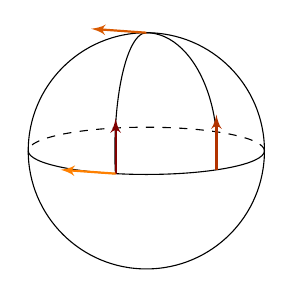
\begin{tikzpicture}
    \draw circle [radius=1.5];

    \draw (1.5, 0) arc(0:-180:1.5 and 0.3);
    \draw [dashed] (1.5, 0) arc(0:180:1.5 and 0.3);

    \draw (0, 1.5) arc(90:191:0.4 and 1.5);

    \draw (0, 1.5) arc(90:-9:0.9 and 1.5);

    \draw [mred, thick, -latex'] (-0.39, -0.29) -- +(0, 0.7);
    \draw [mred!60!morange, thick, -latex'] (0.89, -0.24) -- +(0, 0.7);

    \draw [mred!30!morange, -latex', thick] (0, 1.5) -- +(-0.7, 0.05);

    \draw [morange, -latex', thick] (-0.39, -0.29) -- +(-0.7, 0.05);
  \end{tikzpicture}
\end{center} % improve picture
We see that after the parallel transport around the loop, we get a \emph{different} vector. It is in this sense that the connection on $S^2$ is not flat.

Thus, what we want is the following notion:
\begin{defi}[Parallel vector field]\index{parallel vector field}
  We say a vector field $V \in \Vect(M)$ is \emph{parallel} if $V$ is parallel along any curve in $M$.
\end{defi}

\begin{eg}
  In $\R^2$, we can pick $\xi \in T_0\R^2 \cong \R^2$. Then setting $V(p) = \xi \in T_p \R^2 \cong \R^2$ gives a parallel vector field with $V(0) = \xi$.
\end{eg}

However, we cannot find a non-trivial parallel vector field on $S^2$.

This motivates the question --- given a manifold $M$ and a $\xi \in T_p M$ non-zero, does there exist a parallel vector field $V$ on some neighbourhood of $p$ with $V(p) = \xi$?

Naively, we would try to construct it as follows. Say $\dim M = 2$ with coordinates $x, y$. Put $p = (0, 0)$. Then we can transport $\xi$ along the line $\{y = 0\}$ to define $V(x, 0)$. Then for each $\alpha$, we parallel transport $V(\alpha, 0)$ along $\{x = \alpha\}$. So this determines $V(x, y)$.

Now if we want this to work, then $V$ has to be parallel along any curve, and in particular for lines $\{y = \beta\}$ for $\beta \not= 0$. If we stare at it long enough, we figure out a necessary condition is
\[
  \nabla_{\frac{\partial}{\partial x_i}} \nabla_{\frac{\partial}{\partial x_j}} = \nabla_{\frac{\partial}{\partial x_j}} \nabla_{\frac{\partial}{\partial x_i}}.
\]
So the failure of these to commute tells us the curvature. This definition in fact works for any vector bundle.

The actual definition we will state will be slightly funny, but we will soon show afterwards that this is what we think it is.
\begin{defi}[Curvature]\index{curvature}
  The \emph{curvature} of a connection $\d_E: \Omega^0(E) \to \Omega^1(E)$ is the map
  \[
    F_E = \d_E \circ \d_E: \Omega^0(E) \to \Omega^2(E).
  \]
\end{defi}

\begin{lemma}
  $F_E$ is a tensor. In particular, $F_E \in \Omega^2(\End(E))$.
\end{lemma}

\begin{proof}
  We have to show that $F_E$ is linear over $C^\infty(M)$. We let $f \in C^\infty(M)$ and $s \in \Omega^0(E)$. Then we have
  \begin{align*}
    F_E(fs) &= \d_E \d_E (fs)\\
    &= \d_E(\d f \otimes s + f \d_E s)\\
    &= \d^2 f \otimes s - \d f \wedge \d_E s + \d f \wedge \d_E s + f \d_E^2 s\\
    &= f F_E(s) \qedhere
  \end{align*}
\end{proof}

How do we think about this? Given $X, Y \in \Vect(M)$, consider
\begin{align*}
  F_E(X, Y) : \Omega^0(E) &\to \Omega^0(E)\\
  F_E(X, Y)(s) &= (F_E(s))(X, Y)
\end{align*}

\begin{lemma}
  We have
  \[
    F_E(X, Y)(s) = \nabla_X \nabla_Y s - \nabla_Y \nabla_X s - \nabla_{[X, Y]}s.
  \]
  In other words, we have
  \[
    F_E(X, Y) = [\nabla_X, \nabla_Y] - \nabla_{[X, Y]}.
  \]
\end{lemma}
This is what we were talking about, except that we have an extra term $\nabla_{[X, Y]}$, which vanishes in our previous motivating case, since $\frac{\partial}{\partial x_i}$ and $\frac{\partial}{\partial x_j}$ commute in general.

\begin{proof}
  We claim that if $\mu \in \Omega^1(E)$, then we have
  \[
    (\d_E \mu) (X, Y) = \nabla_X (\mu(Y)) - \nabla_Y (\mu(X)) - \mu([X, Y]).
  \]
  To see this, we let $\mu = \omega \otimes s$, where $\omega \in \Omega^1(M)$ and $s \in \Omega^0(E)$. Then we have
  \[
    \d_E \mu = \d \omega \otimes s - \omega \wedge \d_E s.
  \]
  So we know
  \begin{align*}
    (\d_E \mu)(X, Y) &= \d \omega(X, Y) \otimes s - (\omega \wedge \d_E s)(X, Y)\\
    \intertext{By a result in the example sheet, this is equal to}
    &= (X \omega(Y) - Y \omega(X) - \omega([X, Y])) \otimes s \\
    &\quad\quad- \omega(X) \nabla_Y (s) + \omega(Y) \nabla_X(s)\\
    &= X \omega(Y) \otimes s + \omega(Y) \nabla_X s \\
    &\quad \quad- (Y \omega(X) \otimes s + \omega(X) \nabla_Y s) - \omega([X, Y]) \otimes s
  \end{align*}
  Then the claim follows, since
  \begin{align*}
    \mu([X, Y]) &= \omega([X, Y]) \otimes s\\
    \nabla_X(\mu(Y)) &= \nabla_X(\omega(Y) s)\\
    &= X \omega(Y) \otimes s + \omega(Y) \nabla_X s.
  \end{align*}
  Now to prove the lemma, we have
  \begin{align*}
    (F_E s)(X, Y) &= \d_E( \d_E s)(X, Y)\\
    &= \nabla_X((\d_E s)(Y)) - \nabla_Y((\d_E s)(X)) - (\d_E s)([X, Y])\\
    &= \nabla_X \nabla_Y s - \nabla_Y \nabla_X s - \nabla_{[X, Y]} s. \qedhere
  \end{align*}
\end{proof}

\begin{defi}[Flat connection]\index{flat connection}
  A connection $\d_E$ is \emph{flat} if $F_E = 0$.
\end{defi}

Specializing to the Riemannian case, we have
\begin{defi}[Curvature of metric]\index{curvature!of metric}
  Let $(M, g)$ be a Riemannian manifold with metric $g$. The \emph{curvature} of $g$ is the curvature of the Levi-Civita connection, denoted by
  \[
    F_g \in \Omega^2(\End(TM)) = \Omega^0(\Lambda^2 T^* M \otimes TM \otimes T^*M).
  \]
\end{defi}

\begin{defi}[Flat metric]\index{flat metric}
  A Riemannian manifold $(M, g)$ is \emph{flat} if $F_g = 0$.
\end{defi}

Since flatness is a local property, it is clear that if a manifold is locally isometric to $\R^n$, then it is flat. What we want to prove is the converse --- if you are flat, then you are locally isometric to $\R^n$. For completeness, let's define what an isometry is.

\begin{defi}[Isometry]\index{isometry}
  Let $(M, g)$ and $(N, g')$ be Riemannian manifolds. We say $G \in C^\infty(M, N)$ is an \emph{isometry} if $G$ is a diffeomorphism and $G^* g' = g$, i.e.
  \[
    \D G|_p: T_p M \to T_{G(p)} N
  \]
  is an isometry for all $p \in M$.
\end{defi}

\begin{defi}[Locally isometric]\index{locally isometric}
  A manifold $M$ is \emph{locally isometric} to $N$ if for all $p \in M$, there is a neighbourhood $U$ of $p$ and a $V \subseteq N$ and an isometry $G: U \to V$.
\end{defi}

\begin{eg}
  The flat torus obtained by the quotient of $\R^2$ by $\Z^2$ is locally isometric to $\R^2$, but is not diffeomorphic (since it is not even homeomorphic).
\end{eg}

Our goal is to prove the following result.
\begin{thm}
  Let $M$ be a manifold with Riemannian metric $g$ .Then $M$ is flat iff it is locally isometric to $\R^n$.
\end{thm}

One direction is obvious. Since flatness is a local property, we know that if $M$ is locally isometric to $\R^n$, then it is flat.

To prove the remaining of the theorem, we need some preparation.
\begin{prop}
  Let $\dim M = n$ and $U \subseteq M$ open. Let $V_1, \cdots, V_n \in \Vect(U)$ be such that
  \begin{enumerate}
    \item For all $p \in U$, we know $V_1(p), \cdots, V_n(p)$ is a basis for $T_pM$, i.e.\ the $V_i$ are a frame.
    \item $[V_i, V_j] = 0$, i.e.\ the $V_i$ form a frame that pairwise commutes.
  \end{enumerate}
  Then for all $p \in U$, there exists coordinates $x_1, \cdots, x_n$ on a chart $p \in U_p$ such that
  \[
    V_i = \frac{\partial}{\partial x_i}.
  \]
  Suppose that $g$ is a Riemannian metric on $M$ and the $V_i$ are orthonormal in $T_pM$. Then the map defined above is an isometry.
\end{prop}

\begin{proof}
  We fix $p \in U$. Let $\Theta_i$ be the flow of $V_i$. From example sheet 2, we know that since the Lie brackets vanish, the $\Theta_i$ commute.

  Recall that $(\Theta_i)_t(q) = \gamma(t)$, where $\gamma$ is the maximal integral curve of $V_i$ through $q$. Consider
  \[
    \alpha(t_1, \cdots, t_n) = (\Theta_n)_{t_n} \circ (\Theta_{n - 1})_{t_{n - 1}} \circ \cdots \circ (\Theta_1)_{t_1}(p).
  \]
  Now since each of $\Theta_i$ is defined on some small neighbourhood of $p$, so if we just move a bit in each direction, we know that $\alpha$ will be defined for $(t_0, \cdots, t_n) \in B = \{|t_i| < \varepsilon\}$ for some small $\varepsilon$.

  Our next claim is that
  \[
    \D\alpha\left(\frac{\partial}{\partial t_i}\right) = V_i
  \]
  whenever this is defined. Indeed, for $\mathbf{t} \in B$ and $f \in C^\infty(M, \R)$. Then we have
  \begin{align*}
    \D\alpha \left(\left.\frac{\partial}{\partial t_i}\right|_t\right)(f) &= \left.\frac{\partial}{\partial t_i}\right|_t f(\alpha(t_1, \cdots, t_n))\\
    &= \left.\frac{\partial}{\partial t_i} \right|_{\mathbf{t}} f((\Theta_i)_t \circ (\Theta_n)_{t_n} \circ \cdots \circ \widehat{(\Theta_i)_{t_i}} \circ \cdots \circ (\Theta_1)_{t_1}(p))\\
    &= V_i|_{\alpha(\mathbf{t})}(f).
  \end{align*}
  So done. In particular, we have
  \[
    \D \alpha|_0 \left(\left.\frac{\partial}{\partial t_i}\right|_0\right) = V_i(p),
  \]
  and this is a basis for $T_p M$. So $\D \alpha|_0: T_0 \R^n \to T_p M$ is an isomorphism. By the inverse function theorem, this is a local diffeomorphism, and in this chart, the claim tells us that
  \[
    V_i = \frac{\partial}{\partial x_i}.
  \]
  The second part with a Riemannian metric is clear.
\end{proof}

We now actually prove the theorem
\begin{proof}[Proof of theorem]
  Let $(M, g)$ be a flat manifold. We fix $p \in M$. We let $x_1, \cdots, x_n$ be coordinates centered at $p_1$, say defined for $|x_i| < 1$. We need to construct orthonormal vector fields. To do this, we pick an orthonormal basis at a point, and parallel transport it around.

  We let $e_1, \cdots, e_n$ be an orthonormal basis for $T_p M$. We construct vector fields $E_1, \cdots, E_n \in \Vect(U)$ by parallel transport. We first parallel transport along $(x_1, 0, \cdots, 0)$ which defines $E_i(x_1, 0, \cdots, 0)$, then parallel transport along the $x_2$ direction to cover all $E_i(x_1, x_2, 0, \cdots, 0)$ etc, until we define on all of $U$. By construction, we have
  \[
    \nabla_k E_i = 0\tag{$*$}
  \]
  on $\{x_{k + 1} = \cdots = x_n = 0\}$.

  We will show that the $\{E_i\}$ are orthonormal and $[E_i, E_j] = 0$ for all $i, j$. We claim that each $E_i$ is parallel, i.e.\ for any curve $\gamma$, we have
  \[
    \D_\gamma E_i = 0.
  \]
  It is sufficient to prove that
  \[
    \nabla_{j} E_i = 0
  \]
  for all $i, j$.

  By induction on $k$, we show
  \[
    \nabla_{j} E_i = 0
  \]
  for $j \leq k$ on $\{x_{k + 1} = \cdots = x_n = 0\}$. The statement for $k = 1$ is already given by $(*)$. We assume the statement for $k$, so
  \[
    \nabla_j E_i = 0\tag{$A$}
  \]
  for $j \leq k$ and $\{x_{k + 1} = \cdots = x_n = 0\}$. For $j = k + 1$, we know that $\nabla_{k + 1} E_i = 0$ on $\{x_{k + 2} = \cdots = x_n = 0\}$ by $(*)$. So the only problem we have is for $j = k$ and $\{x_{k + 2} = \cdots = x_n = 0\}$.

  By flatness of the Levi-Civita connection, we have
  \[
    \left[\nabla_{k + 1}, \nabla_k\right] = \nabla_{[\partial_{k + 1}, \partial_k]} = 0.
  \]
  So we know
  \[
    \nabla_{k + 1} \nabla_k E_i = \nabla_k \nabla_{k + 1} E_i = 0\tag{$B$}
  \]
  on $\{x_{k + 2} = \cdots = x_n = 0\}$. Now at $x_{k + 1} = 0$ , we know $\nabla_k E_i$ vanishes. So it follows from parallel transport that $\nabla_k E_i$ vanishes on $\{x_{k + 2} = \cdots = x_n = 0\}$.

  As the Levi-Civita connection is compatible with $g$, we know that parallel transport is an isometry. So the inner product product $g(E_i, E_j) = g(e_i, e_j) = \delta_{ij}$. So this gives an orthonormal frame at all points.

  Finally, since the torsion vanishes, we know
  \[
    [E_i, E_j] = \nabla_{E_i} E_j - \nabla_{E_j} E_i = 0,
  \]
  as the $E_i$ are parallel. So we are done by the proposition.
\end{proof}

What does the curvature mean when it is non-zero? There are many answers to this, and we will only give one.

\begin{defi}[Holonomy]\index{holonomy}
  Consider a piecewise smooth curve $\gamma: [0, 1] \to M$ with $\gamma(0) = \gamma(1) = p$. Say we have a linear connection $\nabla$. Then we have a notion of parallel transport along $\gamma$.

  The \emph{holonomy} of $\nabla$ around $\gamma$: is the map
  \[
    H: T_p M \to T_p M
  \]
  given by
  \[
    H(\xi) = V(1),
  \]
  where $V$ is the parallel transport of $\xi$ along $\gamma$.
\end{defi}

\begin{eg}
  If $\nabla$ is compatible with a Riemannian metric $g$, then $H$ is an isometry.
\end{eg}

\begin{eg}
  Consider $\R^n$ with the usual connection. Then if $\xi \in T_0\R^n$, then $H(\xi) = \xi$ for any such path $\gamma$. So the holonomy is trivial.
\end{eg}

\begin{eg}
  Say $(M, g)$ is flat, and $p \in M$. We have seen that there exists a neighbourhood of $p$ such that $(U, g|_U)$ is isometric to $\R^n$. So if $\gamma([0, 1]) \in U$, then $H = \id$.
\end{eg}

The curvature measures the extent to which this does not happen. Suppose we have coordinates $x_1, \cdots, x_n$ on some $(M, g)$. Consider $\gamma$ as follows:
\begin{center}
  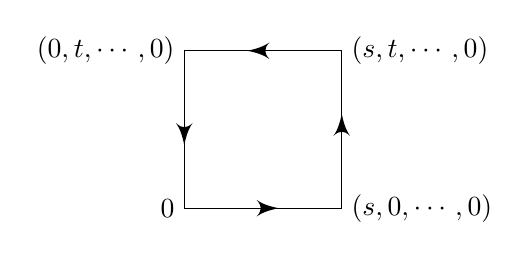
\begin{tikzpicture}
    \draw [->-=0.6] (0, 0) -- (2, 0) node [right] {$(s, 0 , \cdots, 0)$};
    \draw [->-=0.6] (2, 0) -- (2, 2) node [right] {$(s, t, \cdots, 0)$};
    \draw [->-=0.6] (2, 2) -- (0, 2) node [left] {$(0, t, \cdots, 0)$};
    \draw [->-=0.6] (0, 2) -- (0, 0) node [left] {$0$};
  \end{tikzpicture}
\end{center}
Then we can Taylor expand to find
\[
  H = \id + F_g\left(\left.\frac{\partial}{\partial x_1}\right|_p, \left.\frac{\partial}{\partial x_2}\right|_p\right)st + O(s^2 t, st^2).
\]

\printindex
\end{document}
